% !TEX TS-program = pdflatexmk
% !TEX spellcheck = language_tag
\documentclass[fleqn,usenatbib]{mnras}


\usepackage[T1]{fontenc}
\usepackage{ulem}
\usepackage{graphicx}
\usepackage{newtxtext}
\usepackage{amsmath}
\usepackage{amssymb}
\usepackage{hyperref}
\usepackage{multirow}
%\usepackage{natbib}
%\usepackage{float}
\usepackage{color}
\usepackage{ae,aecompl}
\hypersetup{
     colorlinks   = true,
     citecolor    = cyan,
     linkcolor    = cyan
}
%\usepackage{authblk}
%\usepackage{caption}
\usepackage[toc,page]{appendix}
\usepackage{xspace}

% SHORCUTS
\newcommand{\ud}{\ensuremath{\mathrm{d}}}
\newcommand{\helium}{$\mathrm{He^{4}}$\xspace}
\newcommand{\nickel}{$\mathrm{Ni^{56}}$\xspace}
\newcommand{\tracer}{$\mathrm{X}$\xspace}
\newcommand{\iron}{$\mathrm{Fe^{56}}$\xspace}
\newcommand{\cobalt}{$\mathrm{Co^{56}}$\xspace}
\newcommand{\solr}{\xspace\ensuremath{\rm{R_{\odot}}}}
\newcommand{\solm}{\xspace\ensuremath{\rm{M_{\odot}}}}
\newcommand{\kms}{$\mathrm{km/s}$\xspace}
\newcommand{\prom}{\textsc{P{\footnotesize ROMETHEUS}-H{\footnotesize OT}B}\xspace}
\newcommand{\vertexprom}{\textsc{V{\footnotesize ERTEX}-P{\footnotesize ROMETHEUS}}\xspace}
\newcommand{\vertex}{\textsc{V{\footnotesize ERTEX}}\xspace}
\newcommand{\nada}{\textsc{NADA-FLD}\xspace}
\newcommand{\rns}{$R_{\mathrm{ns}}$\xspace\xspace}
\newcommand{\mns}{$M_{\mathrm{ns}}$\xspace\xspace}
\newcommand{\rsh}{$R_{\mathrm{s}}$\xspace\xspace}
\newcommand{\rrevsh}{$R_{\mathrm{revs}}$\xspace\xspace}
\newcommand{\rgain}{$R_{\mathrm{gain}}$\xspace\xspace}

%keeping track of changes
\newcommand{\NY}[2]{{\color{blue}\sout{#1}#2}}
\newcommand{\COM}[1]{{\color{red}#1}}

\title{\NY{Low Mass Core Collapse}{ Supernovae} \NY{}{from Low-Mass Progenitors}}

\author[G. Stockinger et. al]{Georg Stockinger$^1$, H.-T. Janka$^1$, T. Ertl$^1$\\
% institutions
$^1$Max-Planck Institue for Astrophysics}

\date{Released 2019 Xxxxx XX}

% Enter the current year, for the copyright statements etc.
\pubyear{2019}

\begin{document}
\maketitle
\pagerange{\pageref{firstpage}--\pageref{lastpage}} \pubyear{2019}

\begin{abstract}
We \NY{firstly}{} present the results of \NY{fully three dimensional}{ full $4\pi\mathord{-}$3D,} long term \NY{}{BE MORE SPECIFIC} simulations of core-collapse supernova\NY{e}{} (CCSN) \NY{}{resulting} from \NY{two}{} low mass \NY{iron core}{} progenitors.\NY{,}{} \NY{}{We consider two low-mass iron core progenitors} with zero \NY{}{metallicity} \NY{($z9.6$)}{ and} solar metallicity \NY{($s9.0$) respectively}{ which explode as CCSN}, and one progenitor with an oxygen-neon-magnesium core \NY{}{(ONeMg)} \NY{($e8.8$) exploding}{ which explodes} as an electron-capture supernova (ECSN). \NY{We find that}{ In the ECSN case,} \NY{the}{} mixing of Nickel into the envelope is strongly suppressed \NY{in the ECSN case}{} due to \NY{the}{ a} steep density gradient at the outer \NY{}{core} boundary \NY{of its core}{}. The \NY{structural}{} similarity between the \NY{}{core structure of} zero-metallicity progenitor and the ONeMg progenitor \NY{is mirrored}{ leads to similarities} in \NY{the}{ their} explosion properties\NY{,}{.} \NY{}{In both these cases, we observe roughly equal} amount of nickel mixing and \NY{}{qualitatively similar}{} ejecta morphology at late times\NY{, showing only}{(marked by} small \NY{}{deviations from spherical symmetry} \NY{asymmetries}{)}. In \NY{contrary}{ contrast,} the solar metallicity iron core progenitor shows strong growth of Rayleigh-Taylor plumes \NY{over}{ in} the \NY{whole}{ entire} helium core\NY{}{.} \NY{and stronger}{ The strong} initial asymmetries \NY{leading}{ leads} to \NY{far}{} more pronounced mixing\NY{}{.} \NY{and a}{ In this case the} final morphology \NY{more}{ is remarkably} similar to \NY{structures also found}{ the remnant morphology seen in} \NY{the}{} long term simulation\NY{}{s} of \NY{more}{} massive progenitors. 

\end{abstract}

\begin{keywords}
Core-collapse --- hydrodynamics
\NY{}{MORE KEYWORDS (TAKE THEM FROM A PAPER BY ANOOP}
\end{keywords}
\noindent

\section{ToDo}
\begin{itemize}
    \item Mass distribution plots wspace/hspace
    \item $s9.0$ multi D description
    \item Comparison other works
    \item Description 1D shorter ?
\end{itemize}

\section{Introduction}
\NY{}{COMMENT: 1.Use shorter sentences 2. Use citealt when you cite a lot of works inside (see e.g. blah-blah-blah). 3. When citing multiple papers they should go in a time order.}

\NY{The explosion of stars with a birth mass more massive than 8\solm is triggered by the collapse of the inner core initializing a shock wave that runs through the envelope and eventually reaching the surface.}{ According to current understanding stars with mass $\mathord{\gtrsim}\,8\, \solm$ end their lives in a core-collapse supernova. The explosion is powered by gravitational energy, which is released when core of the star collapses.} \NY{Since the first theoretical approaches, of these core-collapse supernova (CCSNe) events by \citet{Colgate_1966} many }{ In the last six decades numerous} studies \NY{}{have} focused on the collapse \NY{}{phase} and subsequent evolution \NY{first in one dimension}{ using 1D simulations.} \NY{and more recently}{ Over the last two decades, 2D simulations with better micro-physics inputs have driven our understanding of the core-collapse problem (CITE SOMEONE). A close study of these models has lead to the discovery of new hydrodynamic instabilities such as standing accretion shock instability (SASI) (CITE SOMEONE).} \NY{and only}{ The increase in computational capabilities in the recent years along with new developments in neutrino transport algorithms (CITE SOME)has resulted} in full \NY{three dimensions}{ 3D simulations} (see e.g. \citealt{Melson2015}, \citealt{Vartanyan2018}). Motivated by the famous SN1987A and its progenitor detection, some studies (e.g. \citealt{Mueller1991}, \citealt{Kifonidis2003}, \citealt{Hammer2009}, \citealt{Wongwathanarat}) also investigated the propagation of the shock wave beyond the shock breakout with models in mass range of 15-20\solm, suitable as progenitors for SN1987A, in two and three dimensions. 
These theoretical works showed that supernova explosions are by far not a spherical event as previously thought. Three dimensional effects may even facilitate explosions \cite{Muellera}, \cite{Melson2015}) and are a necessary ingredient to explain the clumpiness and mixing found in spectral analyses of the nebular phase of core collapse events (\cite{Jerkstrand2011}). 
\NY{Further, studies by}{} \citet{Wongwathanarat_2013} \NY{also showed}{ show} that the final ejecta distribution \NY{still}{} carries imprint\NY{s}{} \NY{by}{ of} the 
asphericities \NY{that evolved}{ produced} during the explosion \NY{phase} ($\NY{}{t}\,\mathord{\sim}\, 1\, \rm s$)\NY{}{,} \NY{}{which are further amplified} \NY{but is strongly altered}{} during later phases. \NY{In dependence}{ Depending} on the detailed progenitor structure, \NY{}{hydrodynamic instabilities arising at the composition interfaces, such as the} Rayleigh-Taylor \NY{}{instability}(RTI) \NY{and other  instabilities arising at the composition interfaces}{} will shape the final \NY{}{spatial and velocity} distribution \NY{and velocities of metals}{of nucleosynthetic products}. \NY{Results vary from almost}{ The resulting ejecta morphology ranges} homogenously shaped ejecta to strongly pronounced RT-fingers resembling also the  distribution found in Cas A. Due to the highly complex and stochastic behaviour of turbulence during the explosion phase and nonlinear evolution of the RTI a clear connection between the asymmetries, and thus the amount of mixing, and the progenitor structure hard to draw.

\NY{Considering}{ For progenitors with} lower \NY{initial}{} masses\NY{, ranging from}{ between} \NY{$\sim$ 8 to 10\solm}{ $8\mathord{-}10\, \solm$,} where\NY{, considering a standard Salpeter initial mass function,}{} up to 40\% of all CCSNe are thought to occur \NY{}{(assuming Salpeter initial mass function  \citep{Salpeter_1955})}, these differences may \NY{be even more extreme}{ become more important}. 

The evolution of stars with mass $\mathord{\lesssim}\,12\, \solm$ is very sensitive to the initial mass \citep{Woosley2015}.
Even the critical mass division points, if they really exist in this monotonic definition (\cite{Woosley2015}), where progenitors evolve into CO and ONe white dwarfs ($\mathrm{M_{up}}$), ONeMg cores ($\mathrm{M_{n}}$) and iron cores ($\mathrm{M_{mass}}$) is still under debate. 
The critical mass needed to form an iron core at the center $\mathrm{M_{mass}}$ is found to be around 9\solm but is shifted by almost 2\solm depending on overshooting and mass loss prescriptions \cite{Siess2007}. 
For $\mathrm{M_{up}}$ values in the literature vary between 7.5-9\solm (\cite{Poelarends2008},  \cite{Siess2007EvolutionAGBstars}). For $\mathrm{M_{n}}$ values are less wide spread from 8.7\solm (\cite{Jones2013}) and 8.8\solm \cite{Nomoto1984EvolutionCores}.

\NY{A special example of these complexities is the 8.8\solm electron-capture supernova (ECSN) progenitor of \cite{Nomoto1984}}{ The $8.8\, \solm$ progenitor of \cite{Nomoto1984} is even more peculiar}. \NY{The star}{ It} \NY{evolves}{ experiences} \NY{through}{} several thermal pulses and off-center ignition of fusion material\NY{}{.} \NY{into}{ In the end, it has} a degenerate \NY{oxygen-magnesium-neon (ONeMg)}{ ONeMg} core \NY{with}{ surrounded by} a dilute and \NY{very}{ an} extended hydrogen envelope.
%The collapse of this core is triggered by electron captures on $\mathrm{^{20}Ne}$ and $\mathrm{^{24}Mg}$ (hence the name ECSN). 
During their evolution they are able to burn carbon at the center first as a convectively bounded flame (CBF) followed by carbon shell burning. As a result a degenerate ONeMg core grows at the center of the star until it reaches its Chandrasekhar mass. At this point electron captures on $\mathrm{^{24}Mg}$ via the reactions $\mathrm{^{24}Mg(e^-,\nu_e)}^{24}\mathrm{Na}$  and $\mathrm{^{24}Mg(e^-,\nu_e)}^{24}\mathrm{Ne}$ destabilize the core due to the reduction of electron-degeneracy pressure. Continuous $e^-$-capture on $\mathrm{^{20}Ne}$ that further reduces supporting pressure works against the now beginning oxygen-burning as temperatures increase during the collapse. Simulations in 1D (see e.g. \cite{NihonTenmonGakkai.1949PublicationsJapan.}, \cite{Janka2008}, \cite{Kitaura2006}) suggest that the collapse proceeds despite the oxygen burning. \cite{Jones2016} simulated the deflagration of oxygen in ONeMg cores with different core densities. Below $\log_{10}\rho_c=10.3$ their core do not collapse but get partly unbound due to the inefficient \NY{semiconvective}{ semi-convective} mixing during the electron capture phase and the resulting strong thermonuclear runaway. Only when central densities are higher than $\rho_c$ the core is found to collapse to a neutron star.
Despite the narrow mass range and competing processes that depend strongly on the employed physics, some suggestions for ECSNe  are SN 1994N, 1997D, 1999br, 1999eu, 2011dc and 2005cs (\cite{StevensonExtremeBlasts}). Although in discrepancy with previous results by \cite{Gessner2018HydrodynamicalSupernova} concerning the maximum kick velocity of neutron stars produced by ECSNe, also SN1054 (the Crab) has been suggested to be an ECSN.
Above $\mathrm{M_{mass}}$ stars go through a phase of oxygen and silicon burning that is longer in comparison with their more massive ($M > 15\, \solm$) counterparts.  This can lead to additional mass loss in the last decade of evolution or even to single mass ejection events when burning flames reach the surface of the star before collapse (\cite{Woosley2015}).

\NY{With these differences in mind this study is focused on the following questions}{ In this work we attempt to investigate the following questions:}
\begin{itemize}
\item \NY{Are there decisive}{ What are the major} differences between the long term evolution of \NY{}{an} ECSNe and \NY{}{a} CCSNe\NY{}{?}
\item \NY{If so, what}{ What} is the influence of the progenitor structure \NY{ON WHAT??} 
\item Can these differences be detected without detailed spectral analysis
\end {itemize}

\section{Progenitors}
% pre collapse 
\NY{We}{ In this paper, we} study \NY{the explosion and long term evolution of}{} an \NY{electron capture supernova}{ ECSN} ($e8.8$) and \NY{the long term evolution of}{} two \NY{}{CCSNe resulting from} low mass iron core \NY{single star}{} progenitors ($z9.6$, $s9.0$). \NY{The}{ In case of the ECSN we study both} explosion \NY{}{and the long term evolution} \NY{of the ECSN model is explored here firstly}{,} whereas \NY{}{for the CCSNe we study only the long term evolution.} \NY{the}{ The} explosion of \NY{the more massive}{ iron core} progenitors \NY{was conducted by}{ has been published in} \cite{Melson2015} and \cite{Melson2019}. 

\subsection{ESCN progenitor}
\NY{At the low mass end of our set of progenitors we employ}{ For this study we use} a solar metallicity \NY{}{progenitor with} $M_{\rm ZAMS}\mathord{=}8.8\,\solm$ \NY{progenitor, provided by}{ from} Nomoto (2017)\NY{,}{.} \NY{with}{ This progenitor has} an ONeMg core\NY{}{,} \NY{that}{ which} explodes as an \NY{electron capture supernova}{ ECSN}. \NY{A a commonly used quantitative measure to describe the}{ The} density structure of \NY{the}{ a} \NY{pre-SN}{ progenitor} model \NY{is  the}{ can be quantified using the} compactness parameter \citep{Oconnor2011}\NY{}{,} \NY{}{which is defined as}
\begin{equation}
\label{equ:compactness}
  \xi_{M} \equiv \frac{M/\solm}{R(M_{\rm bary}=M)/10^{3}\, \rm km},
\end{equation}
where \NY{$R(M_{\rm bary}=M)$}{ $R$} is the \NY{radius of the enclosed}{ radial coordinate which encloses} baryonic mass \NY{}{$M$}. The \NY{ECSN}{ ONeMg core} progenitor \NY{}{being studied here} shows very small values of $\xi$ ($\xi_{2.5}=5.7\times10^{-6}$, $\xi_{1.5}=8.0\times10^{-6}$)  representing the sharp density jump outside the core. \NY{Common features of pre-SN models of ECSNe are the very}{ The progenitor model shows} steep density gradient at the \NY{border}{ outer edge} of the ONeMg core\NY{,}{.} \NY{the}{ The core is surrounded by a} very thin \NY{carbon and helium}{ carbon-helium} \NY{layers}{ shell} \NY{with only a few hundreds of a solar mass in total}{ ($M_{\rm C}\,\mathord{\approx}\, 6.80\mathord{\times}10^{-2}\, \solm$, $M_{\rm He}\,\mathord{\sim}\,10^{-5}\, \solm$)} and \NY{the very extended dilute}{ a} hydrogen envelope \NY{}{($M_{\rm H}\,\mathord{\approx}\, 4.36\, \solm$) extending from $INNER\, RADIUS- \mathord{1.19}\mathord{\times}10^{3}\, \solr$}.
Due to this specific structure the progenitor explosions can be triggered even in one dimensional self-consistent simulations \citet{VonGroote, Kitaura2006}. However explosion energies are fairly low with about $10^{50}\;\mathrm{erg}$ in comparison with the fiducial $10^{51}\;\mathrm{erg}$. In our case the $1.332\, \solm$ ONeMg core\footnote{We determine the composition interfaces by the radius at which some element reaches at least half its maximum value. A summary of interface radii and masses is provided in \autoref{tab:progenitors}.} is surrounded by a 0.068\solm thin layer of carbon on which very little helium ($\sim 10^{-5}$\solm) resides. The hydrogen envelope of 4.36\solm extends to $8.3\times10^{13}\;\mathrm{cm}$. 
A previous version of the progenitor, commonly termed $e8.8$ in the literature and $e8.8_{\mathrm{n}}$ in this publication, has been used by various studies, ranging from nucleosynthesis (\cite{Wanajo2018}) to neutron-star kicks (\cite{Gessner2018}) and is a reference case for the simulations of electron capture SNe. Main differences to the previously used progenitor model are the slightly less massive but larger ONeMg core ($\mathrm{\Delta M = 0.0353\solm}$, $R_{\mathrm{ONeMg}}=848.1\;\mathrm{km}$). The final pre-SN mass of the new model is also larger with a more extended hydrogen envelope, see also \autoref{fig:prog_tem_rho_ye_rhor}. The explosion of this progenitor  in this study is modelled with \prom detailed in the next section.
% \begin{figure}
%  \centering
%  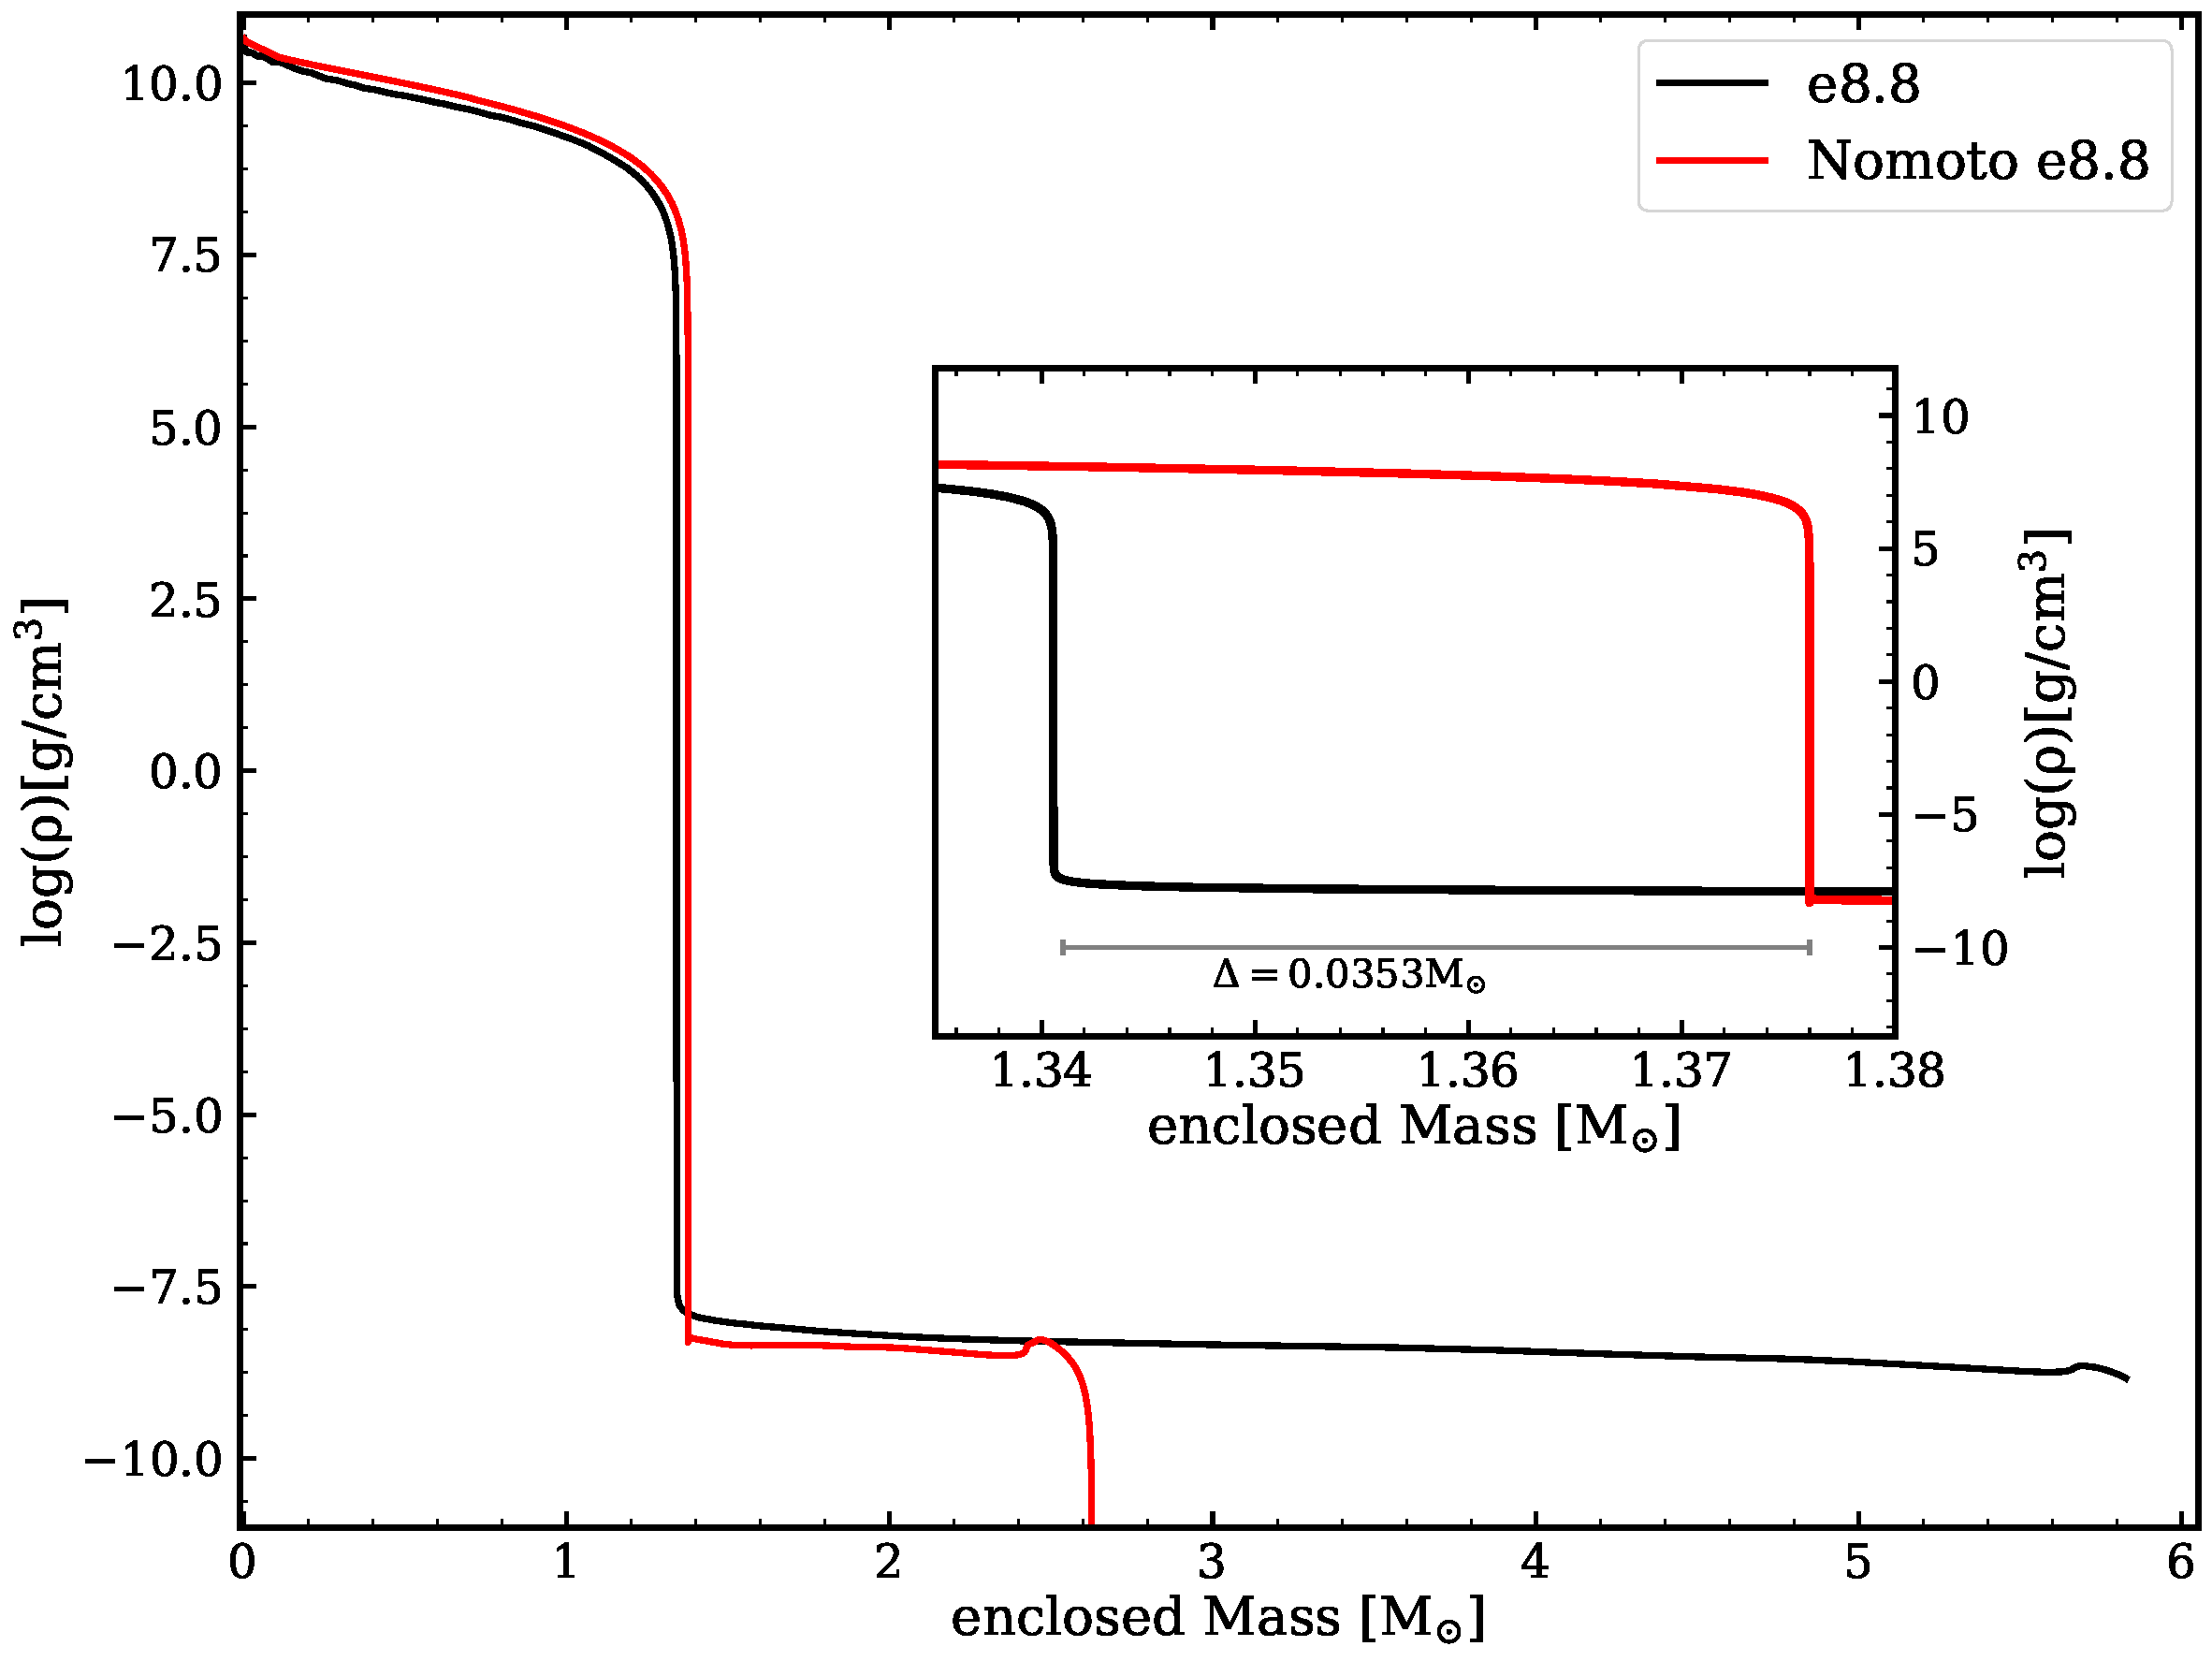
\includegraphics[width=0.4\textwidth]{./pic/e8_nomoto.pdf}
%  \caption{Comparison of the 'old' ECSN-progenitor with the newer version. The previous core extends further out in mass ($\Delta \mathrm{M}\approx 0.0353\solm$)}
%  \label{fig:e8vsnomoto}
% \end{figure}

\subsection{Progenitors for CCSNe}
As a second progenitor in we employ the non-rotating zero metallicity $M_{\mathrm{ZAMS}}$ = 9.6\solm, termed $z9.6$. It was first used by \citet{Janka2012} and is also found in other studies like \citet{Mueller2016,Mueller2018}. This iron-core progenitor is structurally similar to the ECSN model. It also shows a sharp decline of the density outside its core enabling low energetic explosions in 1D. 
Evolved as an extension to \cite{Heger2008} the pre-SN model develops an iron-core of about 1.28\solm with a thin Helium layer of about 0.27\solm below a massive H-Envelope of 8\solm. As the envelope is not polluted by metals, mass loss plays only a minor role during its evolution, leaving the total mass of the star almost unchanged. Similar to the pre-SN state of the ECSN model the $z9.6$ shows low values compactness  parameter $\xi$ ($\xi_{2.5}= 7.65 \times 10^{-5}$, $\xi_{1.5}= 2.37 \times 10^{-4}$). 
Due to its structure it was one of the first iron core progenitors that exploded in fully self consistent simulations by \cite{Melson2015a} with \vertexprom, which is detailed in the next section. This simulation provides the initial state for our investigation. 

Further we investigate a solar metallicity $M_{\mathrm{ZAMS}}$ = 9.0\solm star, termed $s9.0$, provided by Heger (2013) that has slightly larger compactness values as the previous models ($\xi_{2.5}= 3.83 \times 10^{-5}$, $\xi_{1.5}= 5.25 \times 10^{-3}$). Its 1.318\solm Iron core is surrounded by Carbon-Oxygen layer of 0.082\solm on top of which a Helium shell of 0.169\solm resides. The Hydrogen envelope extends from 1.57\solm up to 8.749\solm. 
This progenitor was also chosen to be representative for low-mass CCSNe by \cite{Jerkstrand2017a} who focused on the late time spectral emission of the supernova remnant, and by \cite{Glas2018} focusing on the neutrino emission during the explosion. The three dimensional exploding model for our investigation is provided by T. Melson (2018, not published) and has also been modeled with \vertexprom.

Although the considered progenitors occupy only a very small range of ZAMS mass their structure differs strongly. In Figure \ref{fig:prog_tem_rho_ye_rhor} we show the $\rho r^3$ - profiles of the respective progenitors, alongside the electron fraction $Y_{\mathrm{e}}$, density $\rho$ and temperature $T$ versus enclosed mass and radius, where these differences become obvious. We draw special attention to the $\rho r^3$ profile of the respective progenitors as it yields important information of the propagation of the shock. According to \cite{Sedov1959} positive gradients of $\rho r^3$ cause shock deceleration whereas negative gradients cause the opposite. 

The ECSN progenitor exhibits an extremely sharp drop of the $\rho r^3$ profile just outside the ONeMg core. It is this drop in density that enables fast explosions due to the according early rapid drop in mass accretion rate. Outside the core the profile grows monotonically as no more composition interfaces are encountered.  
Similar to the electron capture model the $z9.6$ shows a monotonic $\rho r^3$ outside the CO core where only a small reduction of the density can be seen at the He/H interface.
The $s9.0$ model on the other hand shows strong variations in its $\rho r^3$ - profile. Shells with different compositions are clearly separated by a negative $\rho r^3$ - gradient just before the respective interface. Of particular interest are the CO/He and He/H interfaces. These will have an impact on the long term evolution of the explosion as will be discussed in Section \ref{subsec:LinearStabilityAnalysis}.


% \begin{figure}
%  \centering
%  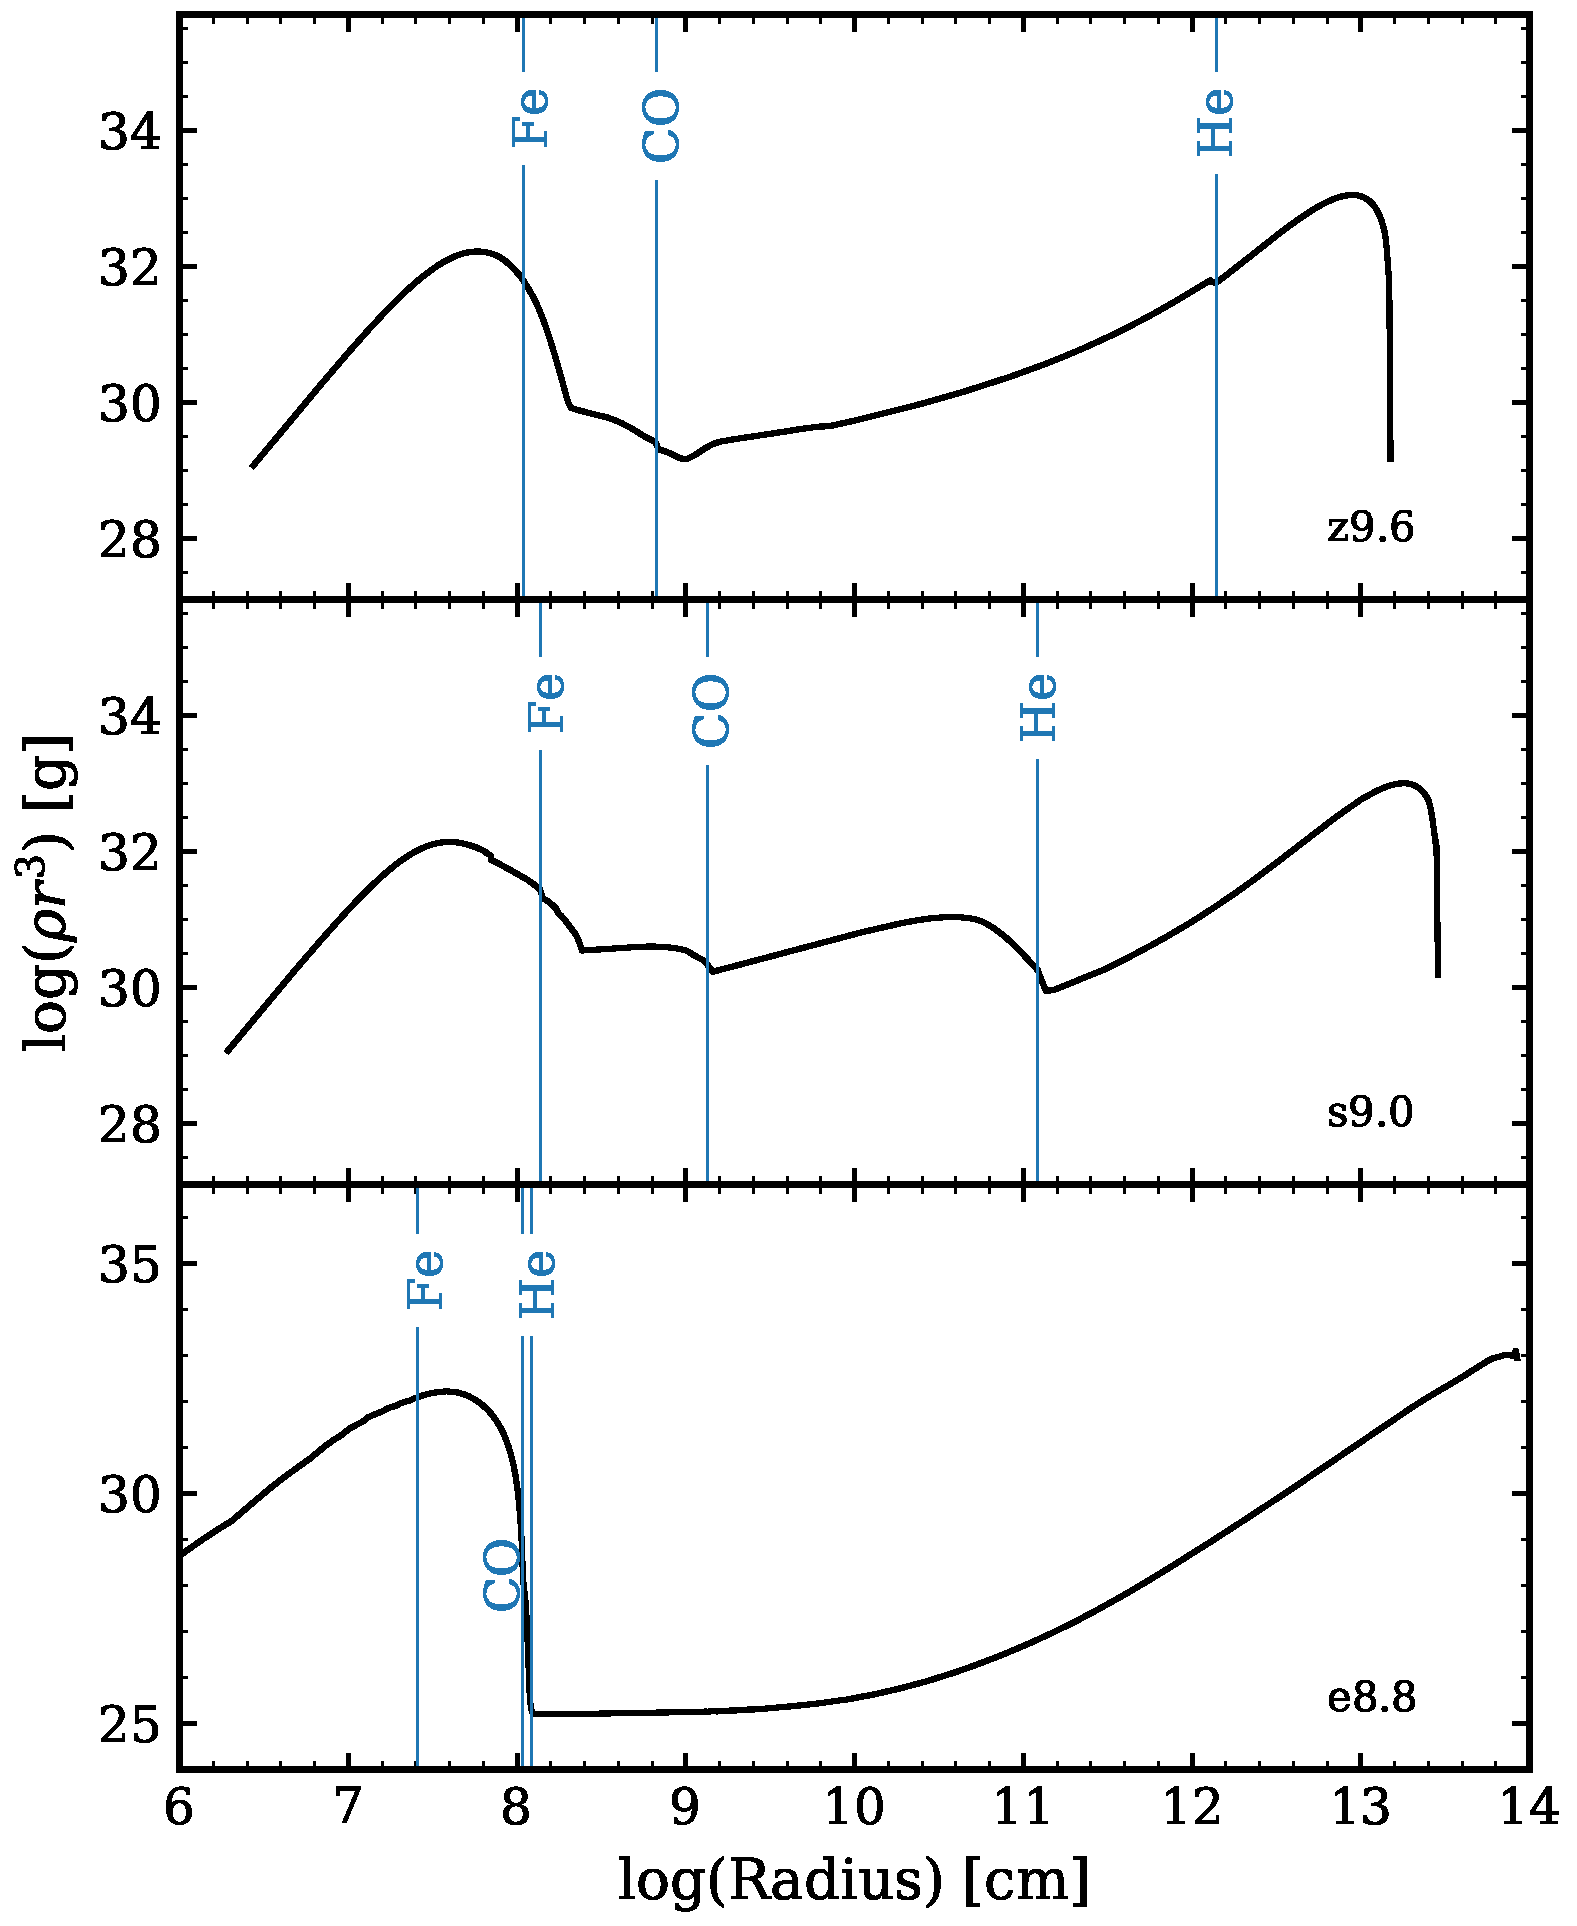
\includegraphics[width=0.49\textwidth]{./pic/rhorcubed_row.pdf}
%  \caption{Progenitor structure of the simulated models. \textit{Top left:} $z9.6$, \textit{Top Right:}$s9.0$, \textit{Bottom Left:} $e8.8$. Black lines show the $\rho r^3$ profile of the respective star. Dashed grey lines denote composition interfaces as labeled in the figure. Note the variability in the $\rho r^3$ profile in the s9.0 Model whereas the $e8.8$ profile is monotonic outside of the CO-core}
%  \label{fig:rho_rcubed_interfaces}
% \end{figure}

\begin{figure*}
 \centering
 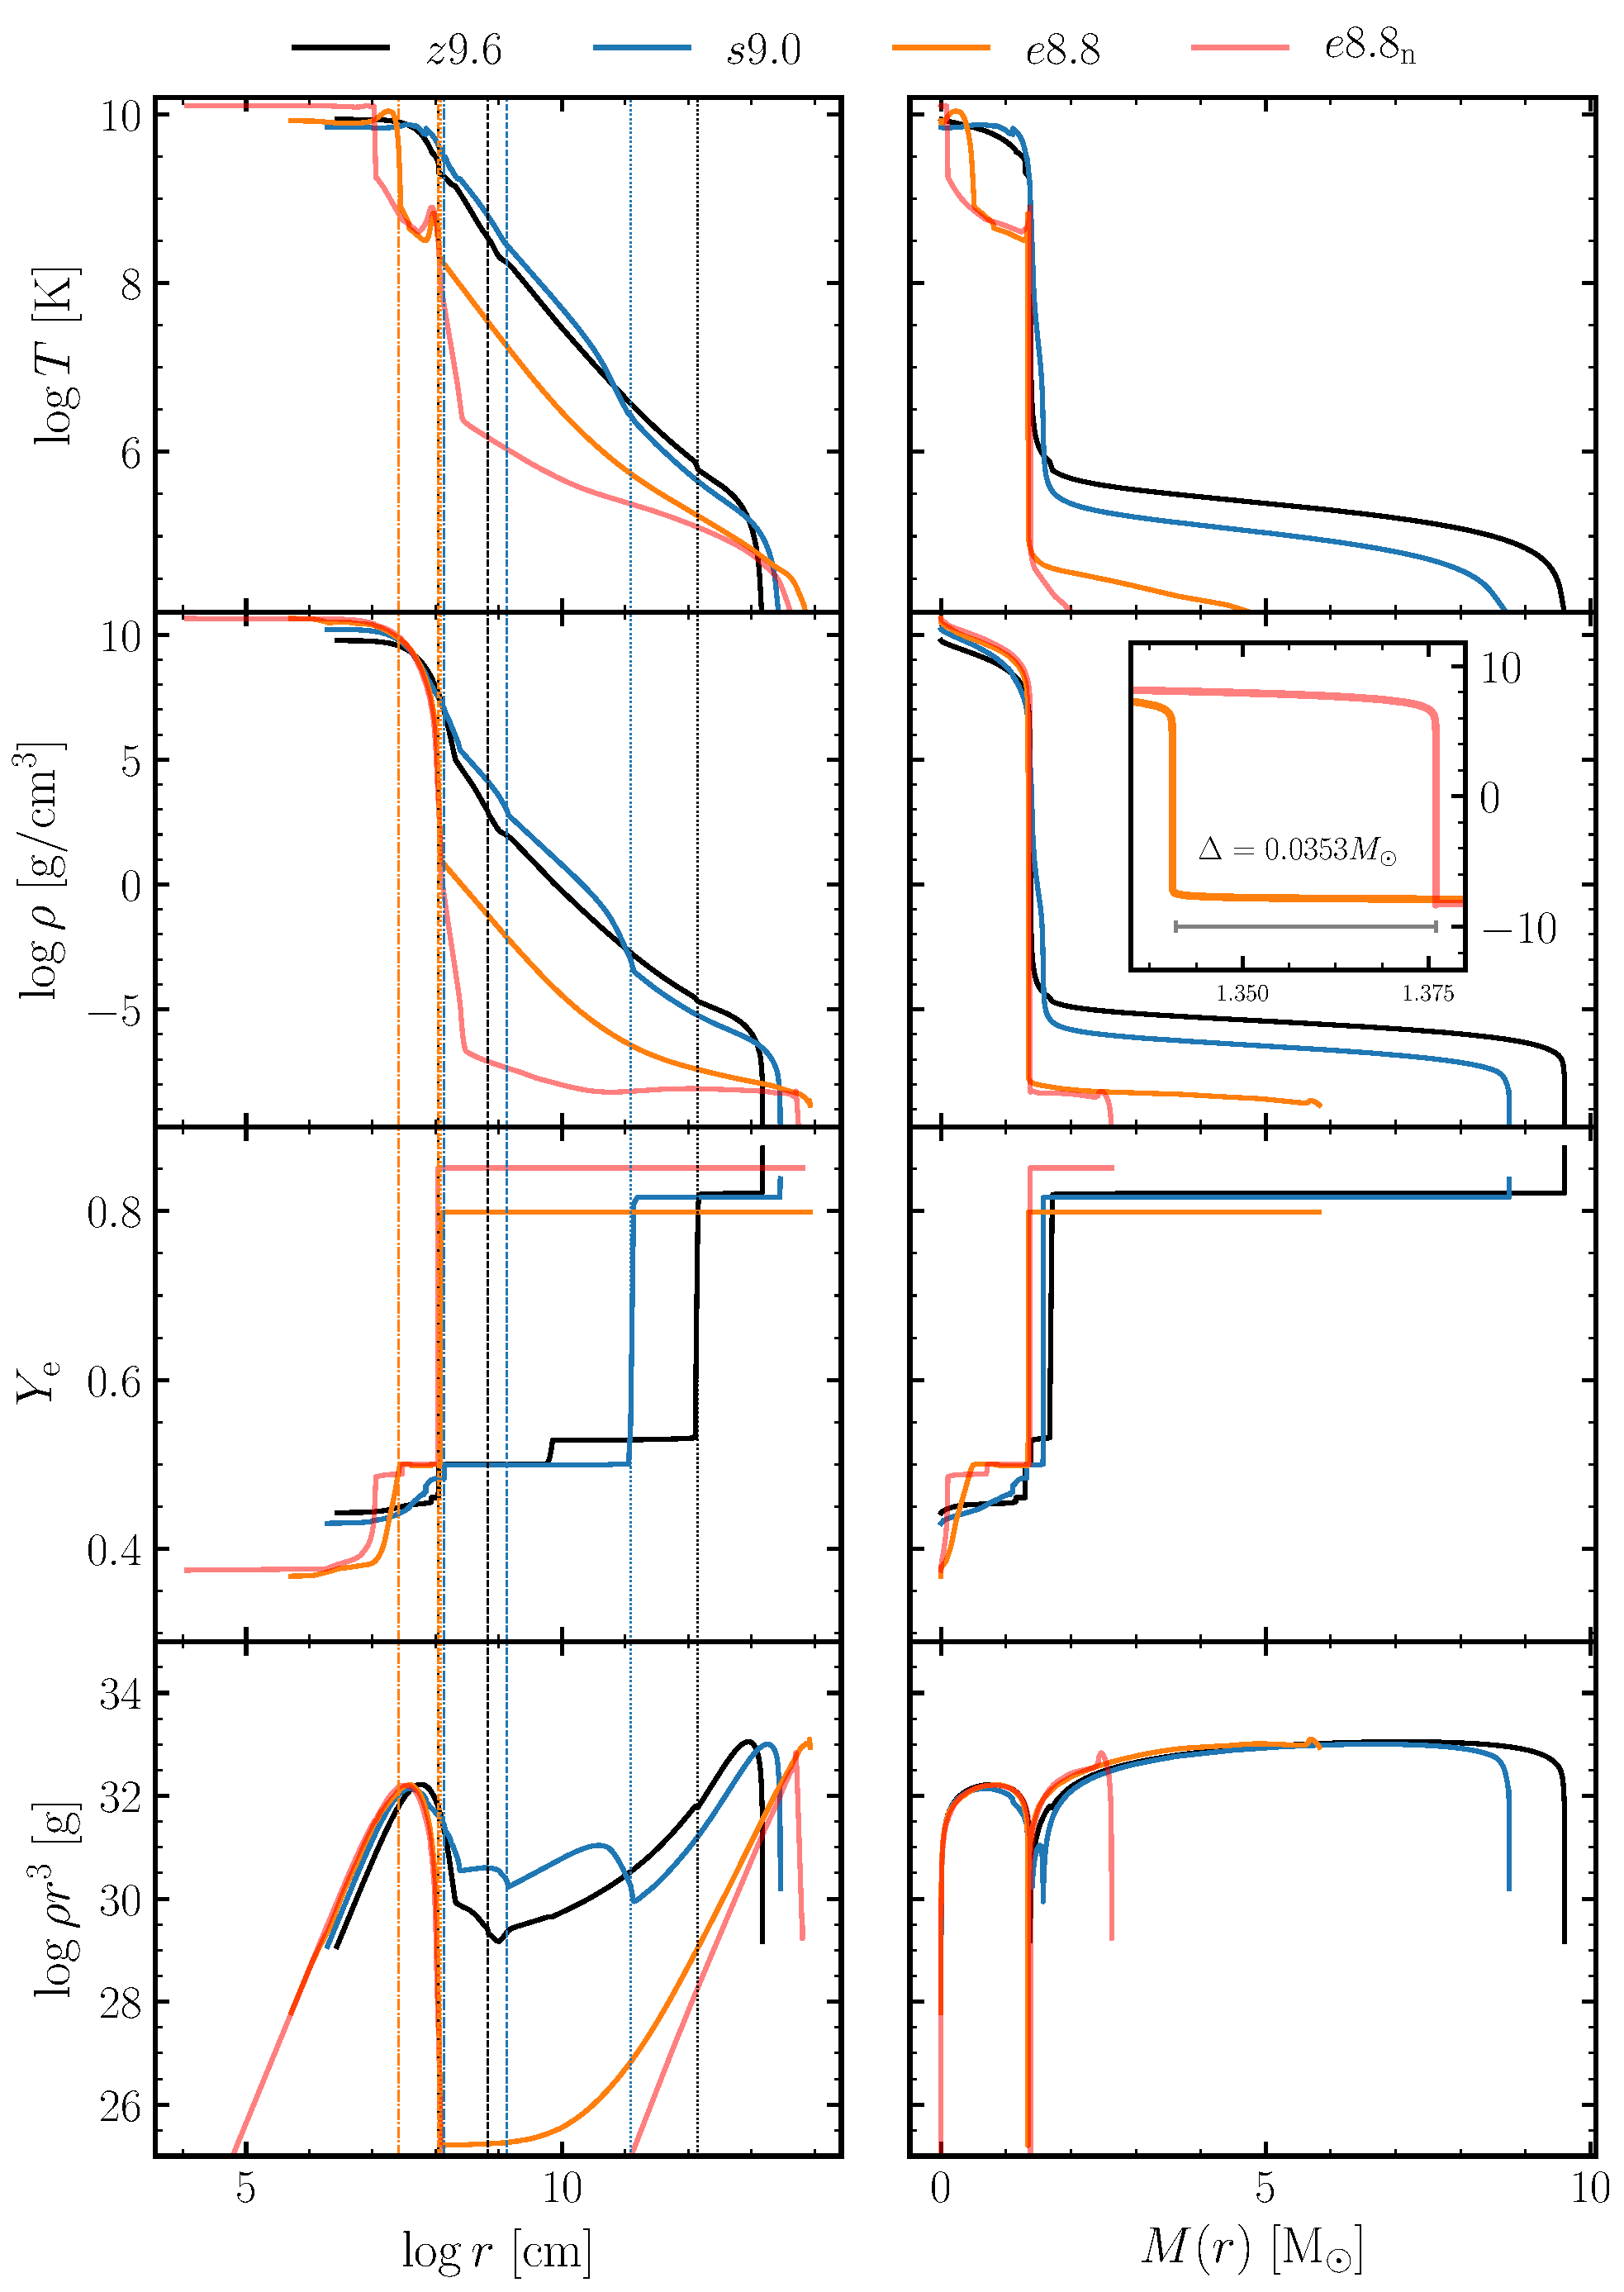
\includegraphics[scale=0.35]{./pic/progenitors_tem_rho_ye_rhor}
 \caption{Profiles of the temperature, density\NY{}{, electron fraction} ($Y_{\text{e}}$) and $\rho r^3$ for the \NY{$z9.6$, $s9.0$, $e8.8$ and $e8.8_{\mathrm{n}}$}{ progenitor models as function of radial coordinate (left panels) and mass coordinate (right panels)}. \NY{The left column shows the quantities over radius whereas the right column shows the same quantities versus enclosed mass}{}. Indicated by dashed, dash-dotted and dotted lines are the outer boundaries of the iron-, CO and He cores respectively. Note the huge differences in the density and $rho r^3$ profiles between the iron and ONeMg cores in particular just outside the CO core. Additionally we show the difference in the core structure between the $e8.8$ and $e8.8_{\mathrm{n}}$ in the $\rho$ over $M(r)$ plot in an inlay.}
 \label{fig:prog_tem_rho_ye_rhor}
\end{figure*}

For this paper we performed spherical-symmetric, axis-symmetric and fully three dimensional simulations for all models beginning from the collapse until the shock reaches the surface of the star. The different setups and approaches for the simulations will be described in the following section.

\section{Numerical and Physical Setup}
\label{sec:explosionModeling}
In order to cover the the collapse, explosion, shock revival and propagation through the envelope and circum-stellar material we employ a step-wise approach.
The collapse phase of the iron core progenitors is modeled with \vertex whereas the ECSN progenitor is collapsed with \prom.
Same applies for the explosion phase, so roughly the first second. \NY{In this study we do not consider progenitor perturbation by Silicon burning for example but use}{ We impose} low amplitude random perturbations \NY{applied}{in the entire simulated region} after bounce \NY{}{in order} to break the spherical symmetry. 
The subsequent long term simulations, covering shock propagation through the star until shock breakout, were conducted with \prom.
In the following \NY{}{sections} we describe \NY{in more detail}{} the physics \NY{applied for}{ implemented} \NY{each code}{} during the different stages of the evolution.

\subsection{Collapse}
The collapse of the iron core progenitors was \NY{handled fully self-consistently with}{ computed using the} \vertex\NY{.}{ code and the collapse} \NY{For the}{ of} electron-capture model was \NY{collapsed with}{ computed using the} \prom\NY{}{ code.} \NY{which}{The \vertex code uses  whereas the \prom} employs \NY{}{the} parametrized scheme \NY{}{for neutrino transport as described} by \citet{Liebendoerfer2005}. The necessary $\rho-Y_{e}$-trajectory was provided by \cite{Huedepohl2018}.
Note that the collapse is performed in one dimension as the initial progenitors are provided in one dimension as well. Additionally any pre-collapse perturbations are frozen in the self similar collapsing core. 

\subsection{Post bounce simulations in Vertex}

\vertexprom  is a finite-volume hydrodynamics code with three-flavor, energy-dependent, ray-by-ray-plus (RbR+) neutrino transport including the full set of neutrino reactions and microphysics as detailed in \cite{Rampp2002}.  The numerical grid employed is the axis-free YinYang-Grid developed by \cite{Kageyama2004} and implemented in \vertexprom by \cite{Melson2015}. It significantly reduces the artifacts of purely spherical grids on the polar axes. 

At high densities above \NY{$\rho_{\mathrm{hd}}=1\times10^{11}\;\mathrm{g/cm^3}$}{$\rho_{\rm{hd}}=10^{11}\;\mathrm{g/cm^3}$} the  Equation of State (EOS) of \cite{Lattimer1991} with a nuclear incompressibility of $\mathrm{K}=220\mathrm{MeV}$ is used. Below $\rho_{\mathrm{hd}}$ \vertexprom employs the low-density EOS of \cite{Janka1999Unpublished}. Above a certain temperature $T_{\mathrm{NSE}}$ nuclear statistical equilibrium is assumed, whereas below that value nuclear reactions are accounted for by a flashing scheme (\cite{Ramppa}) in order to provide an estimate of the nucleosynthetic yields.
Gravity is included as a 1D potential including general-relativistic corrections.

The innermost convectively stable region (up to 10 km) is simulated in 1D. To break the symmetry random perturbations of order $10^{-3}$ were imposed on the density stratification.

\subsection{Post Bounce simulation in Prometheus-HotB}

Different to the iron core progenitors the explosion of the electron-capture progenitor was conducted with \prom (see e.g. \citet{Wongwathanarat2012,Wongwathanarat2013}).
% Nue Transport 
Different to the sophisticated neutrino transport in \vertex, \prom employs a grey transport scheme under the assumption of low neutrino-opacities and calculates the $\nu_{\mathrm{e,x}}$-fluxes by an analytic formula described in detail by \cite{Scheck2006}\footnote{Some improvements of the neutrino transport described in detail in \cite{Scheck2006} are give in the Appendix \ref{Appendix:Neutrino}.}. The details of this scheme are described in the next section.
% Grav
\prom employs a 3D gravitational potential with general relativistic correction by using a multipole expansion of Poisson's equation in its integral form. 
% network
A 17-Species Alpha-Nuclear-Network keeps track of the nucleosynthesis up to $\mathrm{Ni}^{56}$. To follow neutronized matter (with $Y_e < 0.5 $) a tracer species ($X$) with the same binding energy as $\mathrm{Ni}^{56}$ is added to the network. The energy release due to nuclear burning is calculated and enters the energy conservation equation as a source-term. 
The recombination of free neutron and protons up to \helium is included by a flashing scheme.
During later stages the $\beta^{+}$ - decay of radioactive \nickel has to be considered. We therefore add \iron and \cobalt to our set of species and follow their decay via
\begin{equation}
\begin{split}
	_{28} ^{56} \mathrm{Ni}& \rightarrow _{27} ^{56} \mathrm{Co} + e^+ + \nu_e + \gamma \\
	_{27} ^{56} \mathrm{Co}& \rightarrow _{26} ^{56} \mathrm{Fe} + e^+ + \nu_e + \gamma 
\end{split}
\end{equation}
where the $\gamma$'s carry $\Delta E_{\mathrm{\gamma,Ni}} = 1.72\;\mathrm{MeV}$ and $\Delta E_{\mathrm{\gamma,Co}} =3.61\;\mathrm{MeV}$ of the respective reaction whereas the freely escaping neutrinos carry the rest. The deposition of the energy per species $\Delta E_{\mathrm{int, species}}$ over a timestep $\Delta t$ into the surrounding plasma is calculated via
\begin{equation}
\begin{split}
		\Delta E_{\mathrm{int, species}} = \; &  \Delta E_{\gamma,\mathrm{species}} \Big( 1 - e^{-\tau(r)} \Big) \times\\ \; & \frac{X_{\mathrm{species}}}{m_{\mathrm{species}}} \Big( 1 - e^{-\Delta t / t_{1/2}} \Big),
 \end{split}
\end{equation}where $t_{1/2} = 8.764\; \mathrm{days}$ for $^{56}\mathrm{Ni}$ and $t_{1/2} = 77.23\; \mathrm{days}$  for $^{56}\mathrm{Co}$ is the half-time of the respective species and $\tau(r)$ the optical depth for the $\gamma$'s along each radial ray in the medium defined as
\begin{equation}
	\tau(r) = \int_{R^*}^{R_{ib}}\rho(r) \kappa_{\gamma} Y_e(r) dr.
\end{equation}Here $\kappa_{\gamma}=0.06 \;\mathrm{cm^2/g}$ is a constant absorptivity and the integration is carried out from the surface of the star down to the inner boundary. 
After the energy release was calculated and the change of electron fraction due to the emitted positrons was conducted the equation of state is called to update every thermodynamic quantity.
% Eos
To cover the high density achieved during the first stages of an explosion \prom  employs the high density equation of state by \citet{Lattimer1991} for densities above $\rho_{\mathrm{hd}}=10^{11}\;\mathrm{g/cm^3}$. When $\rho<\rho_{\mathrm{hd}}$ we use an extended version of the Helmholtz-EoS by \citet{Timmes1999}. Below the table boundaries of the Helmholtz-EoS ($\mathrm{\rho_{low}}=10^{-10}\mathrm{\;g/cm^3}$, $T_{\mathrm{low}}=10^{4}\mathrm{\;K}$) the equation of state is simplified to include only the contributions of a set of Boltzmann gases and the pressure by radiation. The pressure $p$ and the specific internal energy $e$ are then given by

\begin{equation}
    \label{equ:pressure-boltzmann-radiation}
    p = \frac{1}{3}aT^4 + \frac{\mathrm{k_b}}{\mu \mathrm{m_{H}}} \rho T
\end{equation}
\begin{equation}
    \label{equ:energy-boltzmann-radiation}
    e = \frac{aT^4}{\rho} + \frac{3\mathrm{k_b}}{2\mu \mathrm{m_{H}}} T,
\end{equation}
where $a$, $\mathrm{k_b}$, $\rho$, $T$,$\mathrm{m_{H}}$, $\mu$ are the radiation constant, Boltzmann constant, density temperature, atomic mass unit and mean molecular weight respectively. Note that full ionization is assumed in this approach and radiation pressure clearly dominates in the shocked region.

\subsubsection{Parametrization in Prometheus-HotB}
Modeling in \prom is done in several steps where each time the inner boundary of the numerical grid moves further out in mass to increase the timestep and apply the neutrino transport only to regions where the assumption of low opacities hold ($\tau < 100$).
After core bounce the inner 0.5\solm are excised and replaced by a hydrostatic boundary condition and constant neutrino luminosity $L_{\nu_{e}}$ until the forward shock reaches 1.25\solm only a few milliseconds later. Thereafter the inner boundary is moved to 1.1\solm maintaining the hydrostatic condition but now employing a time dependent Langrangian prescription of the radius enclosing 1.1\solm,  in order to model the contraction of the neutron star .
The movement is described by
\begin{equation}
	R_{\mathrm{ib}}(t) = R_{\mathrm{ib,final}} + (R_{\mathrm{ib,ini}} - R_{\mathrm{ib,final}})\; e^{-t/t_0},
\end{equation}
where $R_{\mathrm{ib,ini}}$ and $R_{\mathrm{ib,final}}$ are the initial and the final radius of the 1.1\solm shell and $t_0$ the timescale for the boundary movement. 
To model the time dependent cooling of the neutron star and thus with it the time dependent neutrino luminosities we use the analytic model of \cite{Ugliano2012}. By equating neutrino losses and $PdV$ work on the neutron star surface with the time derivative of the total energy of the PNS the luminosity is found to be
\begin{equation}
\begin{split}
\label{eqn:lib}
	L_{\mathrm{\nu,tot}} = & - \frac{2}{5} \frac{3\Gamma - 4}{3(\Gamma - 1)} \frac{GM^2_{\mathrm{c}} R_{\mathrm{c}}}{R_{\mathrm{c}}^2} \\
            &  - \frac{3\Gamma - 4} {3(\Gamma - 1)} \frac{aGM_{\mathrm{c}}\Delta m_{\mathrm{acc}}R_\mathrm{c}}{R^2_{\mathrm{c}}}  -\frac{aGM_{\mathrm{c}}\Delta m_{\mathrm{acc}}R_{\mathrm{c}}}{3(\Gamma - 1)R_{\mathrm{c}}}.
\end{split}
\end{equation}

Here $\Gamma = 3$ the the adiabatic index of the core model, $G$ the gravitational constant, $M_{\mathrm{c}}$ the core mass, $a$ an efficiency parameter of the accretion luminosity and $\Delta m_{\mathrm{acc}}$ the mass contained between the PNS radius $R_\mathrm{c}$ and the radius at which the density falls below $\rho=10^{10}\mathrm{g/cm^3}$. 
In the axissymmetric and 3D cases $\Delta m_{\mathrm{acc}}$ is determined from the angle averaged density.
The time evolution of the core radius follows a power-law 
\begin{equation}
	R_{\mathrm{c}}(t) =R_{\mathrm{c,final}} + (R_{\mathrm{c,ini}} - R_{\mathrm{c,final}}) \Big( \frac{t+t_{\mathrm{L}}} {t_{\mathrm{L}}}  \Big)^p,
\end{equation}
where $t_L = 1 \; \mathrm{s}$ and $p < 0$ and  initially $R_{\mathrm{c}} = R_{\mathrm{ib}}$.
In sum $p$, $R_{\mathrm{c,final}}$, $a$, $R_{\mathrm{ib,final}}$ and $t_0$ constitute our set of parameters to firstly approximate the physics of the time evolution of the neutron star and to enable explosions also in 1D.
The calibration of these parameters follows \cite{Ertla} and was repeated for the electron-capture progenitor used in this study to cover a variety of explosion energies.
Note that the studies of \cite{Wongwathanarat2015} and \cite{Gessner2018} used a constant luminosity at the inner boundary. 

\subsection{Numerical Setup during the first second}

The 9.6\solm model was run with an initial radial zoning of 400 grid-points distributed logarithmically up to 10.000 km, which was refined in steps up to 650 zones, and 56/148 zones in the $\theta/\phi$ - direction resulting in 2$^\circ$ resolution.
The 9.0\solm model employs the same radial grid and physics as used in the 9.6\solm case but was run with higher angular resolution of 1$^\circ$.

% resolution in HotB 
In order to model the explosion of the ECSN progenitor one needs to account for the huge density drop outside its core. Thus we choose a logarithmic radial grid with 2000 zones extending from the surface of  the 1.1 \solm shell up to $R_{\mathrm{ob}}=2\times 10^{10}\;\mathrm{cm}$ in our 1D simulations during the first second(s). 
For the three dimensional run we reduce the number of grid cells and the radius of the outer boundary to $R_{\mathrm{ob}}=1\times 10^{9}\;\mathrm{cm}$ adding cells as the forward shock draws closer to the boundary.
Changing the outer boundary does not have any influence on the simulation as there is no sonic contact between the ejecta and the envelope and due to the fast expansion of the shock in the ECSN case. The outer layers will not have reacted to the infall of matter below. 
An angular resolution of $2^{\circ}$ is chosen for the multidimensional simulations of all models during the explosion and in the subsequent long term simulations.
Note that due to the extreme gradients in the ECSN progenitor radial and angular resolution can influence the explosion energy. A more detailed discussion can be found in the appendix.
Similar to \cite{Gessner2018} we restrict the simulation to a 1D gravitational potential as deviations from sphericity will by negligible for the considered progenitor.

\subsection{Extending simulations until shock breakout and beyond}

After the successful explosion the neutron star is encompassed in a low density bubble produced by the forward shock. As mass accretion subsides the still hot neutron star continues to cool via the emission of neutrinos which now interact with the surface layers of the PNS.
These neutrinos deposit some of their energy into the matter and drive an outflow called the neutrino-driven wind. 

Since the neutrino driven wind is leaving the neutron star surface almost spherical it is justified to move our inner grid boundary further out and replace the inner region by a point mass. At the inner boundary we include the hydrodynamic effects of the neutrino-driven wind by injecting density, radial velocity and total energy ($\rho,v_r,e$) trajectories from a long time PNS cooling simulation of the z9.6 model conducted in one dimension by R. Bollig (private communication) with \vertex . This model was chosen since it explodes self-consistently in 1D and the properties of the neutron star do not strongly differ from the terminal values of the $s9.0$ model. In Figure \ref{fig:wind} we show the trajectories used for our long-term simulations.

Thus we map our exploding models (similar to \cite{Wongwathanarat2012} and \cite{Mueller2019}), excising the high density part and account for the neutrino-driven wind at the inner boundary. The cutting radius is determined such that matter above this radius is supersonic throughout. When the density at the new boundary drops below the surrounding matter or the simulated time exceeds the time we are able to inject data from the 1D cooling simulation we switch to an open boundary. 

\begin{figure}
\label{fig:wind}
 \centering
 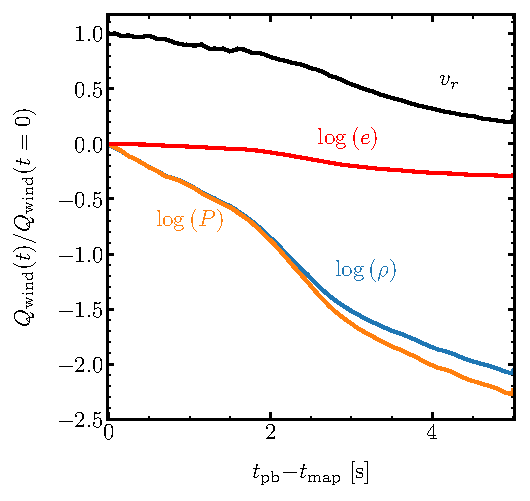
\includegraphics[width=0.45\textwidth]{./pic/wind.pdf}
 \caption{Exemplary trajectories of the radial velocity, total energy density and  density, normalized to their initial values, from the 1D z9.6 model at a radius of 600 km from the time of mapping at $t_{\mathrm{pb}}= 1.4616\;\mathrm{s}$ until $t_{\mathrm{pb}}= 6\;\mathrm{s}$. }
\end{figure}

In order to simulate the shock breakout the progenitor is extended with an atmosphere in hydrostatic equilibrium with the stellar surface. A constant mass loss of $10^{-5}\;\mathrm{M_{\odot}/yr}$ is assumed. 

\subsection{Numerical setup for the long term simulations}

For the long term simulations the radial grid is first extended to the surface of the respective star assuring a radial resolution of better than $1\%$ everywhere. When the forward shock comes close to this outer boundary the grid is extended to $10^{17}\;\mathrm{cm}$ using the stellar wind described in the last section. 

The numerical setup for the iron core progenitors is the same for the extended simulations where only the radius of the stellar surface differs. 

\section{Evolution during the first second}
In the following sections we will present the results of our investigation. We will first provide a detailed analysis of the explosion of the ECSNe progenitor in one- and multi-D and summarize the dynamics of the explosion of the iron-core progenitors conducted by \cite{Melson2015}. 
\subsection{The ECSNe progenitor}
\subsubsection{Shock Propagation and Explosion Properties}
\label{sec:explosion ecsn}

We employ four calibrations as detailed in \autoref{table:e8param} to cover explosion energies, as defined in \autoref{equ:ene exp}, from $3\times 10^{49}\;\mathrm{erg}$ to $1.5\times 10^{50}\;\mathrm{erg}$. These explosion energies are chosen to fit into the ballpark of simulations in the literature conducted with more advanced neutrino treatment and to match observations of SN1054 where kinetic energies of the ejecta are estimated to $\sim 7 \times 10^{49}\;\mathrm{erg}$ \cite{Smith2013}. We simulate post-bounce evolution in one and two dimensions for all calibrations and choose the $e8.8_{10}$ calibration as our reference case in 3 dimensions. 
As our simulations of the electron-capture progenitor resemble the findings of previous studies we will only summarize the main features in the following.

% shock trajectories and energetics 
As already stated by \cite{Janka2008}, the structure of the progenitor is the pivotal element enabling the fast and almost spherical expansion of the forward shock and early rise of explosion energies which are shown in \autoref{fig:eexp}. 
Here we define the explosion energy as the integral over volume elements where the binding energy $e_\mathrm{b}$, which is the sum of the specific internal energy density $e_{\mathrm{int}}$, the specific kinetic energy $e_{\mathrm{kin}}$ and the gravitational potential $\Phi$, is positive\footnote{Note that the given definition of the explosion energy neglects the binding energy of the envelope which is justified as it is a few orders of magnitude less than the energy in the region of interest.}
\begin{equation}
    \mathrm{E}_{\mathrm{exp}} = \int_{e_{\mathrm{b}} > 0} e_{\mathrm{b}} \; \mathrm{dM} =
    \int_{e_{\mathrm{b}} > 0}\; e_{\mathrm{int}} + e_{\mathrm{kin}} + \Phi \; \mathrm{dM}.
    \label{equ:ene exp}
\end{equation}

The sharp drop in density outside the core leads to early plummeting of the mass accretion rate and with it a strong decrease of the ram pressure that typically hinders the shock expansion for several $100\;\mathrm{ms}$. In the ECSN case however the forward shock reaches the core boundary $R_{\mathrm{He/H}}=1010\;\mathrm{km}$, between $t_{\mathrm{pb}}=0.17\;\mathrm{s}$ and $t_{\mathrm{pb}}=0.203\;\mathrm{s}$, depending on the energy input by neutrinos and not on the chosen dimension.

Within this time neutrino heating causes Rayleigh-Taylor bubbles to rise from the vicinity of the nascent neutron star. While the three dimensional simulation develops numerous small scale plumes the axis-symmetric simulations are more dominated by large $l$-mode patterns as can be seen in \autoref{fig:e8 sto 4 times}. These plumes are however unable to influence the propagation of the forward shock as their outermost heads only grew to a few $100 \;\mathrm{km}$ when the shock has already reached some $10^3\;\mathrm{km}$. 
While explosion energies start to rise steeply when the forward shock leaves the ONeMg core, depending on the inner boundary luminosity and retraction of our inner boundary, terminal explosion energies are reached within $t_{\mathrm{pb}}\approx  0.6\;\mathrm{s}$ for the $e8.8_{3}$ model and  $t_{\mathrm{pb}}\approx 1.25\;\mathrm{s}$ in our highest energy case. 

\begin{figure*} % e8.8 2d _3, _10 sto  
 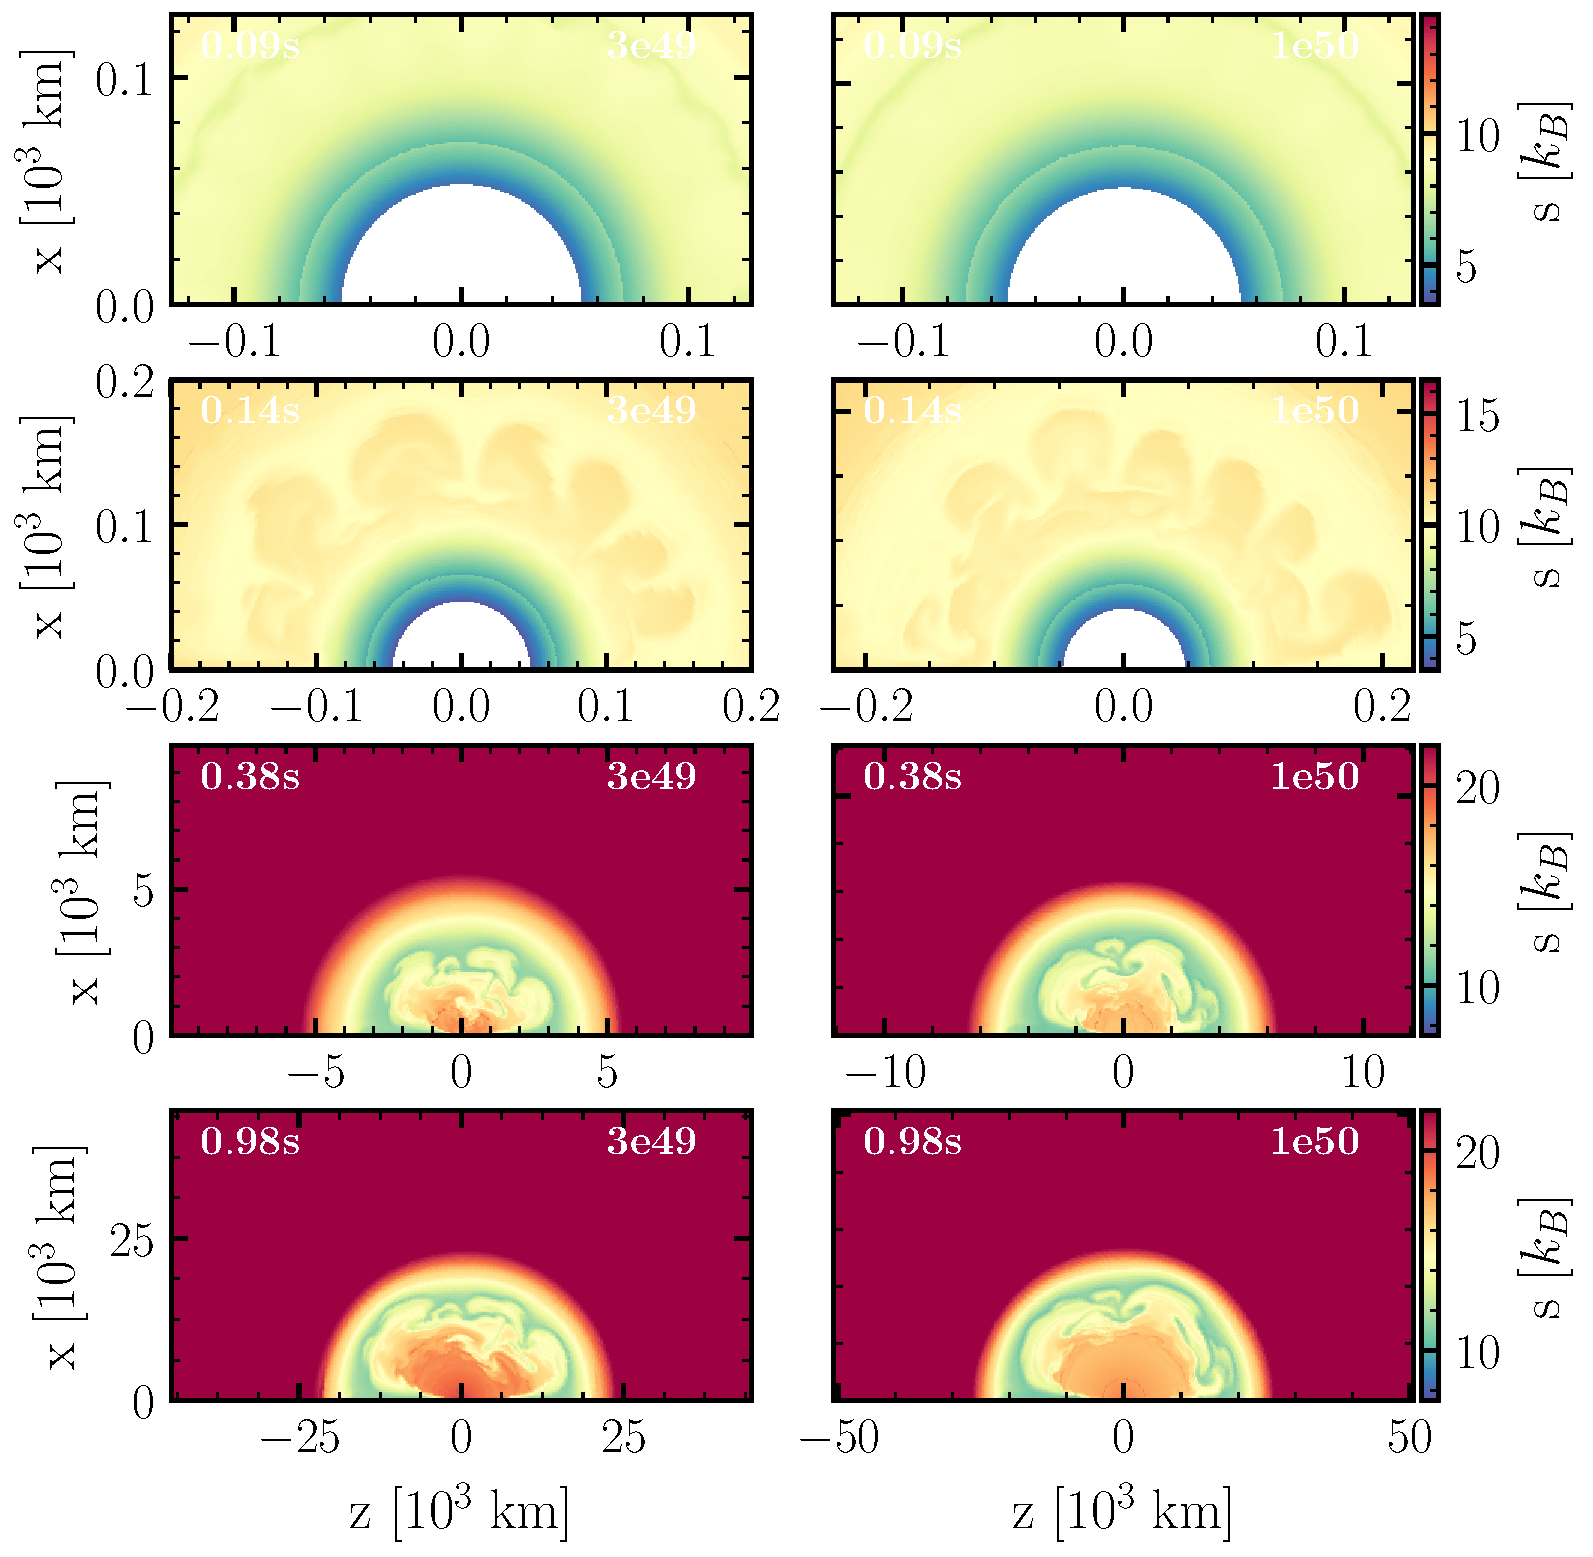
\includegraphics[width=\textwidth]{pic/e8_sto_cuts_2d_1e50_3e49.pdf}
 \caption{Entropy slices of the axis-symmetric $e8.8_{3}$ and  $e8.8_{10}$ simulations at the indicated post-bounce times. Note the similarity in plume size between these models. }
 \label{fig:e8 2d sto times}
\end{figure*}

Note that the qualitative evolution of the first few $100\;\mathrm{ms}$ is basically independent of the chosen dimension or calibration as it is generic for ECSNe. Underlining this we show in \autoref{fig:e8 2d sto times} slices of the entropy of the axis-symmetric $e8.8_{3}$ and $e8.8_{10}$ simulations. Radial and angular sizes of the high entropy plumes are very similar between these two models despite their difference in explosion energy with a factor of 3. 
Minor influences of the chosen symmetry can only be spotted while examining the differences in explosion energy between the spherical and axis symmetric simulations of the $e8.8_{10}$ and $e8.8_{15}$ calibrations. While models with lower explosion energies are basically the same in 1- and 2D, the axis-symmetric simulations with the $e8.8_{10}$ and $e8.8_{15}$ calibrations show slightly smaller explosion energies than their respective spherical symmetric simulation.

% downflows /plumes
This is caused by accretion funnels that are naturally absent in spherical symmetric simulations. 
In the models with high explosion energies the neutron star still accretes matter through these funnels that consequently suppress the emerging neutrino driven wind and thus its energy deposition in the outward moving layers (\cite{Muellera}). Note that hampering of the explosion energy by these persistent downflows is an effect of the chosen geometry. Funnels in axis-symmetric simulations represent a large volume fraction of the whole sphere, whereas in fully three dimensional simulations downflows occupy only a small fraction of the computational domain diminishing their suppressing effect.

As the $\rho r^3$ profile suddenly flattens outside the core the forward shock experiences a massive deceleration sending a pressure wave back into the ejecta. This early deceleration of the forward shock and with it the inner ejecta will have important consequences for the long term evolution of this model which will be described later.

\begin{figure*}
 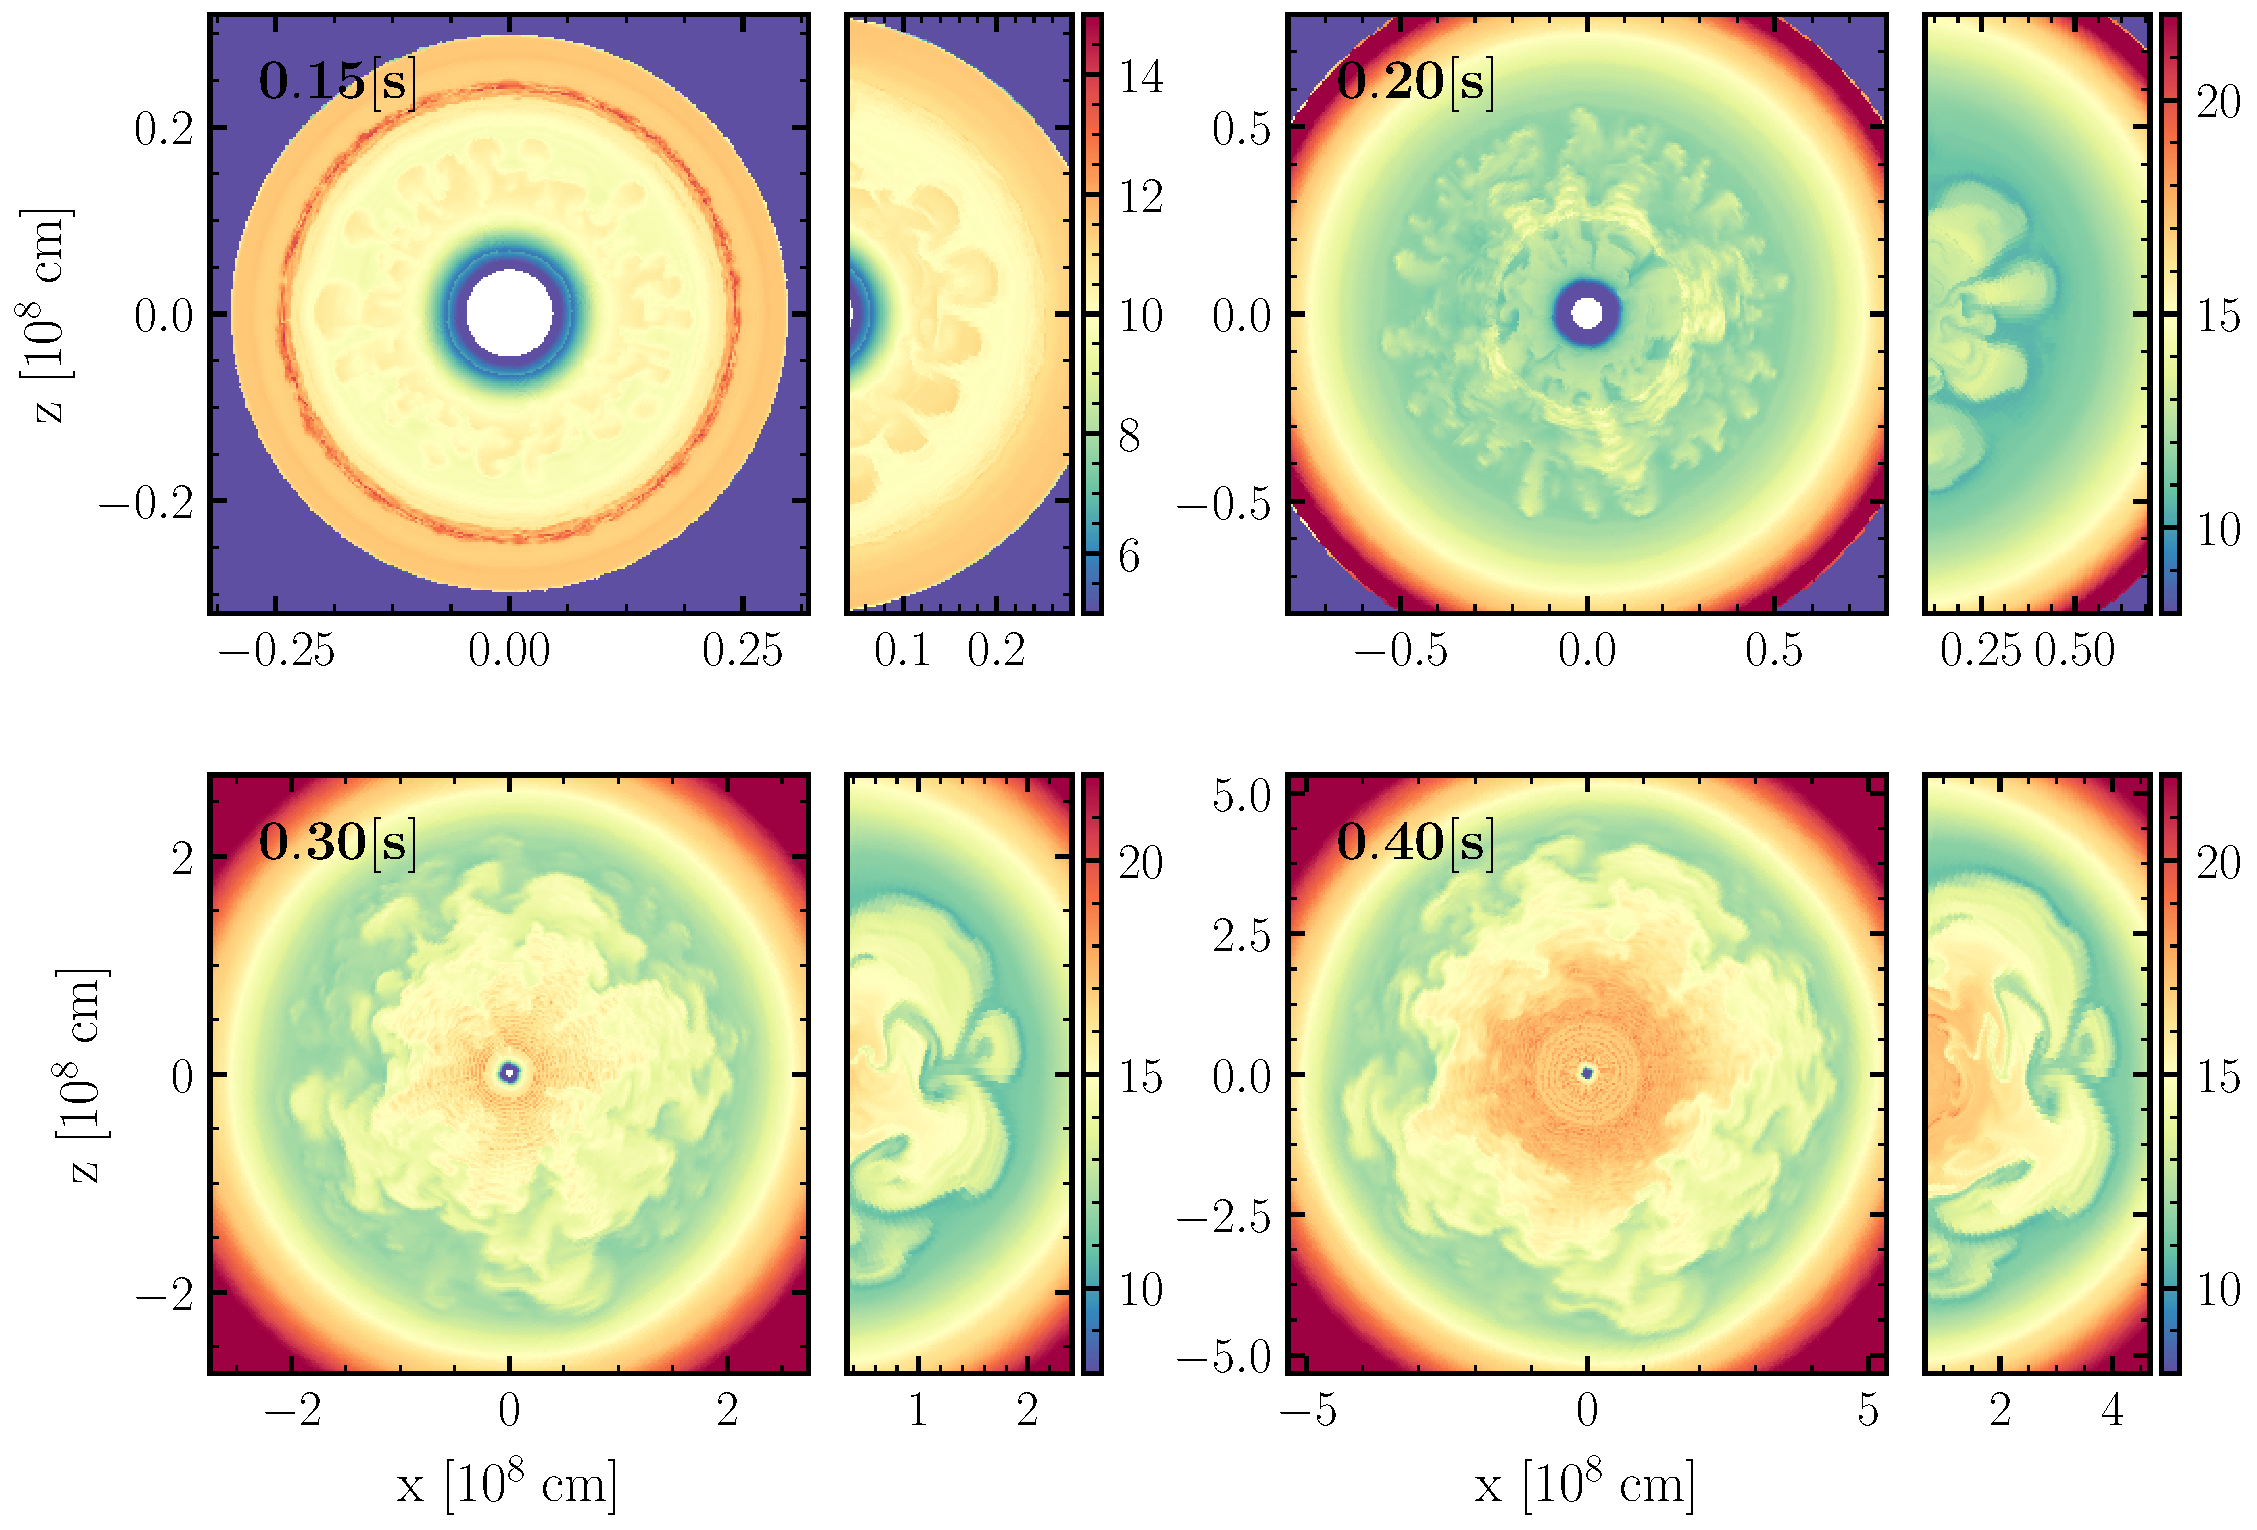
\includegraphics[width=\textwidth]{pic/e8_10_2d3d_sto_cuts_4times.pdf}
 \caption{Entropy slices of the $e8.8_{10}$ model in 3D and 2D at the indicated post-bounce times. }
 \label{fig:e8 sto 4 times}
\end{figure*}


\begin{table}
%\centering
   \begin{tabular}{l| l | l | l | l | l | l}
  \label{table:e8param}
  Name &$E_{\mathrm{exp}}$& p & a & $R_{\mathrm{ib,f}}$ & $t_0$ & $R_{\mathrm{c,f}}$\\
                & [$10^{49}\; \mathrm{erg}$] &   &   & [km]  & [s]& [km] \\
  \hline \hline
  $\mathrm{e}8.8_{3}$ &3 	&	 -3 & 0.01 &27 & 0.1 & 40 \\
  $\mathrm{e}8.8_{6}$ & 6 	& 	-3 & 0.012 &22 & 0.1 & 40 \\
  $\mathrm{e}8.8_{10}$ & 10 	& 	-3 & 0.4 & 20 & 0.1 & 40 \\
  $\mathrm{e}8.8_{15}$ & 15 	& 	-3 & 0.58 & 18 & 0.1 & 40 \\
  \end{tabular}
\caption{Summary of parameters used for the e8.8 Model}
\end{table}

% Comparison to other models
Comparing our results with simulations using a more sophisticated neutrino treatment show only minor differences in the onset of the explosion and rise of the energy. In \cite{Radice2017} positive energies in their baseline model seem to be reached slightly earlier than in our case and grow faster. Also the plateau like feature is missing which could be caused by their definition of the explosion energy where they consider a region with a fixed inner radius at 100 km. The simulations conducted by \cite{Groote2014} and \cite{Janka2008} show very similar behaviour in the evolution of the shock radius $R_{\mathrm{sh}}$ and $E_{\mathrm{exp}}$. 

\begin{figure}
 \centering
 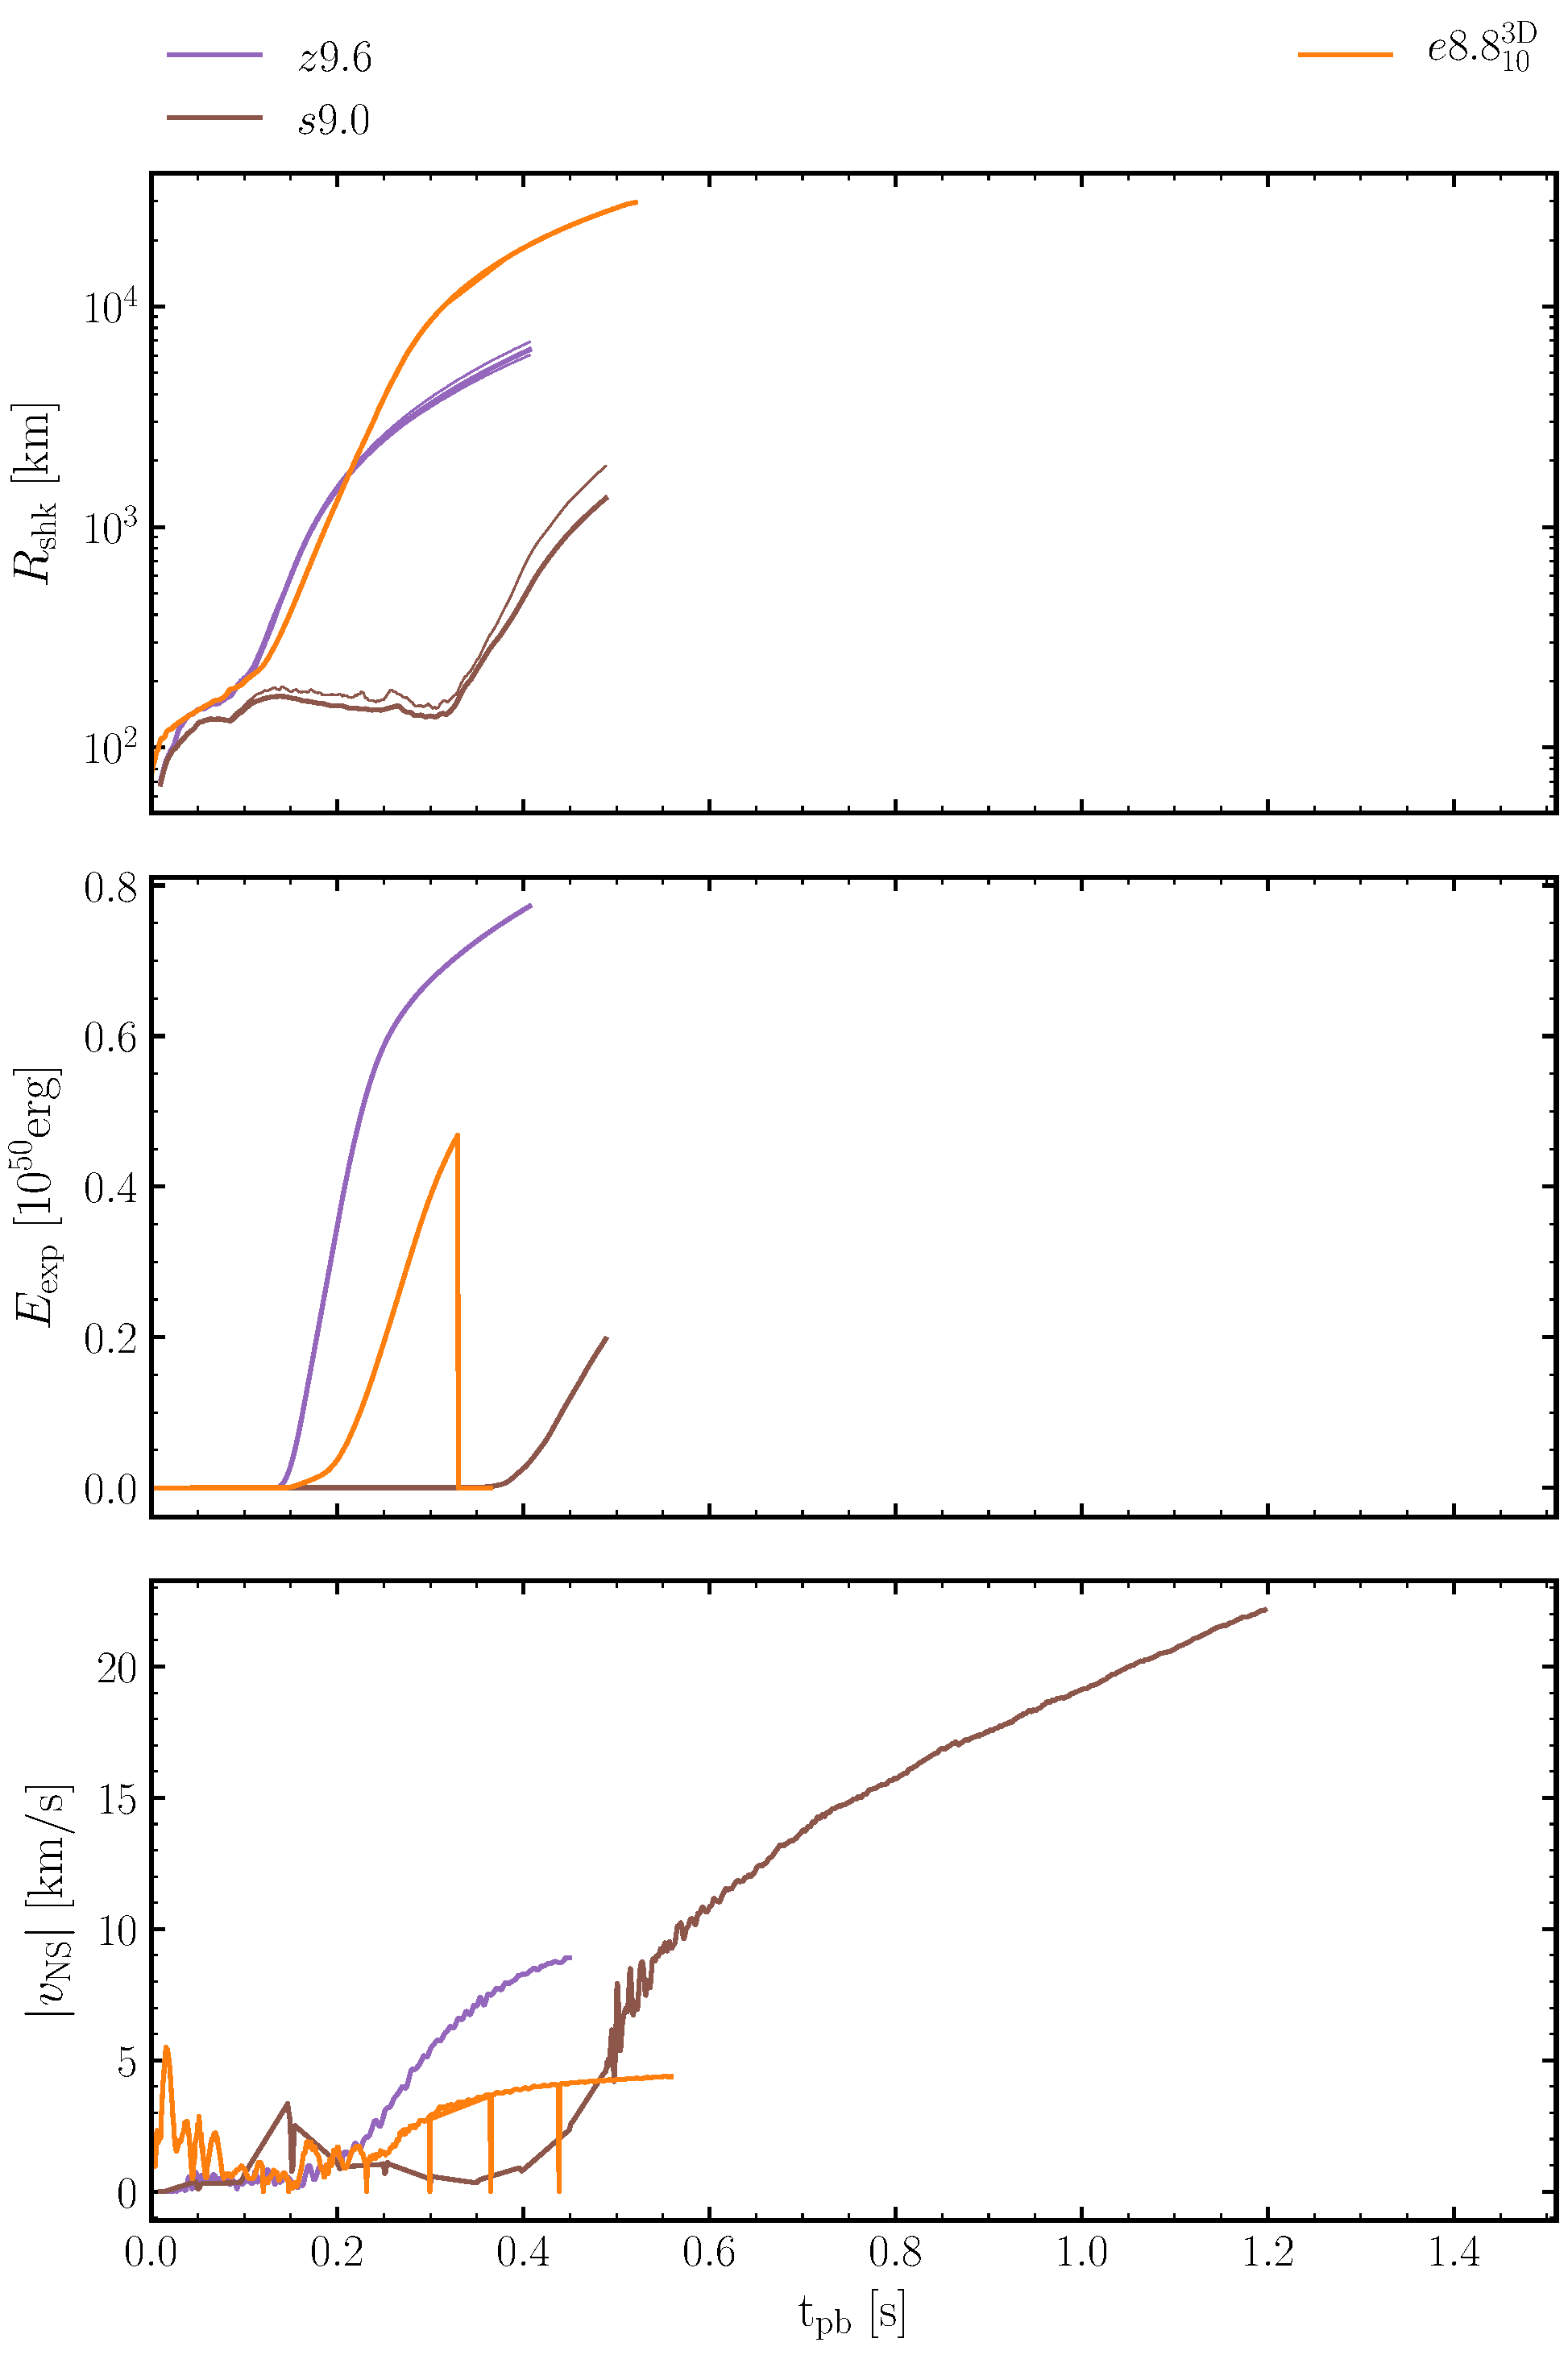
\includegraphics[width=0.49\textwidth]{pic/eexp_shk_kick_all_1d2d3d.pdf}
 \caption{Top Panel: Trajectory of the shock for all our 3D models. Middle Panel: Explosion energies for the respective models. Lower Panel: Hydrodynamic neutron star kick.}
\label{fig:eexp_kick_3D} 
\end{figure}

\subsubsection{Neutron star kicks and spin}
Asphericities that develop during the explosion may exert gravitational forces on the nascent neutron star inducing a 'kick'. What is commonly called the 'gravitational tug-boat' mechanism is the main hydrodynamical cause for neutron star kicks resulting from core collapse supernovae. The evaluation of neutron star kicks from theoretical models provides an interface connecting observations of kick velocities of neutron stars with the asymmetries that developed during the explosion and are not detectable otherwise. Thus we will provide the theoretical neutron star kicks of our models in the following.

Using momentum conservation one can estimate the neutron-star kick via
\begin{equation}
  \pmb{\mathrm{P}}_{\mathrm{gas}} = - \pmb{\mathrm{P}}_{\mathrm{NS}} = - \pmb{\mathrm{v}}_{\mathrm{NS}}\mathrm{M_{NS}},
\end{equation}
where $\mathrm{M_{NS}}$ is the baryonic (neutron star -) mass contained within a radius where the angle-averaged density drops below $\rho = 10^{11} \mathrm{g/cm^3}$, thus giving for the velocity of the NS
\begin{equation}
  \pmb{\mathrm{v}}_{\mathrm{NS}}(t) = - \frac{\pmb{\mathrm{P}}_{\mathrm{gas}}}{ \mathrm{M_{NS}}}.
  \label{equ:momentum_kick}
\end{equation}
The gas momentum is calculated by integrating the total momentum of the matter outside the neutron star via
\begin{equation}
	\label{equ:pz}
  \pmb{\mathrm{P}}_{\mathrm{gas}} (t) = \int_{\mathrm{R_{NS}}}^{\mathrm{R_{ob}}} \rho \pmb{\mathrm{v}} \ud V
\end{equation}

\begin{figure*}
 \label{fig:e8pzkick}
 \centering
 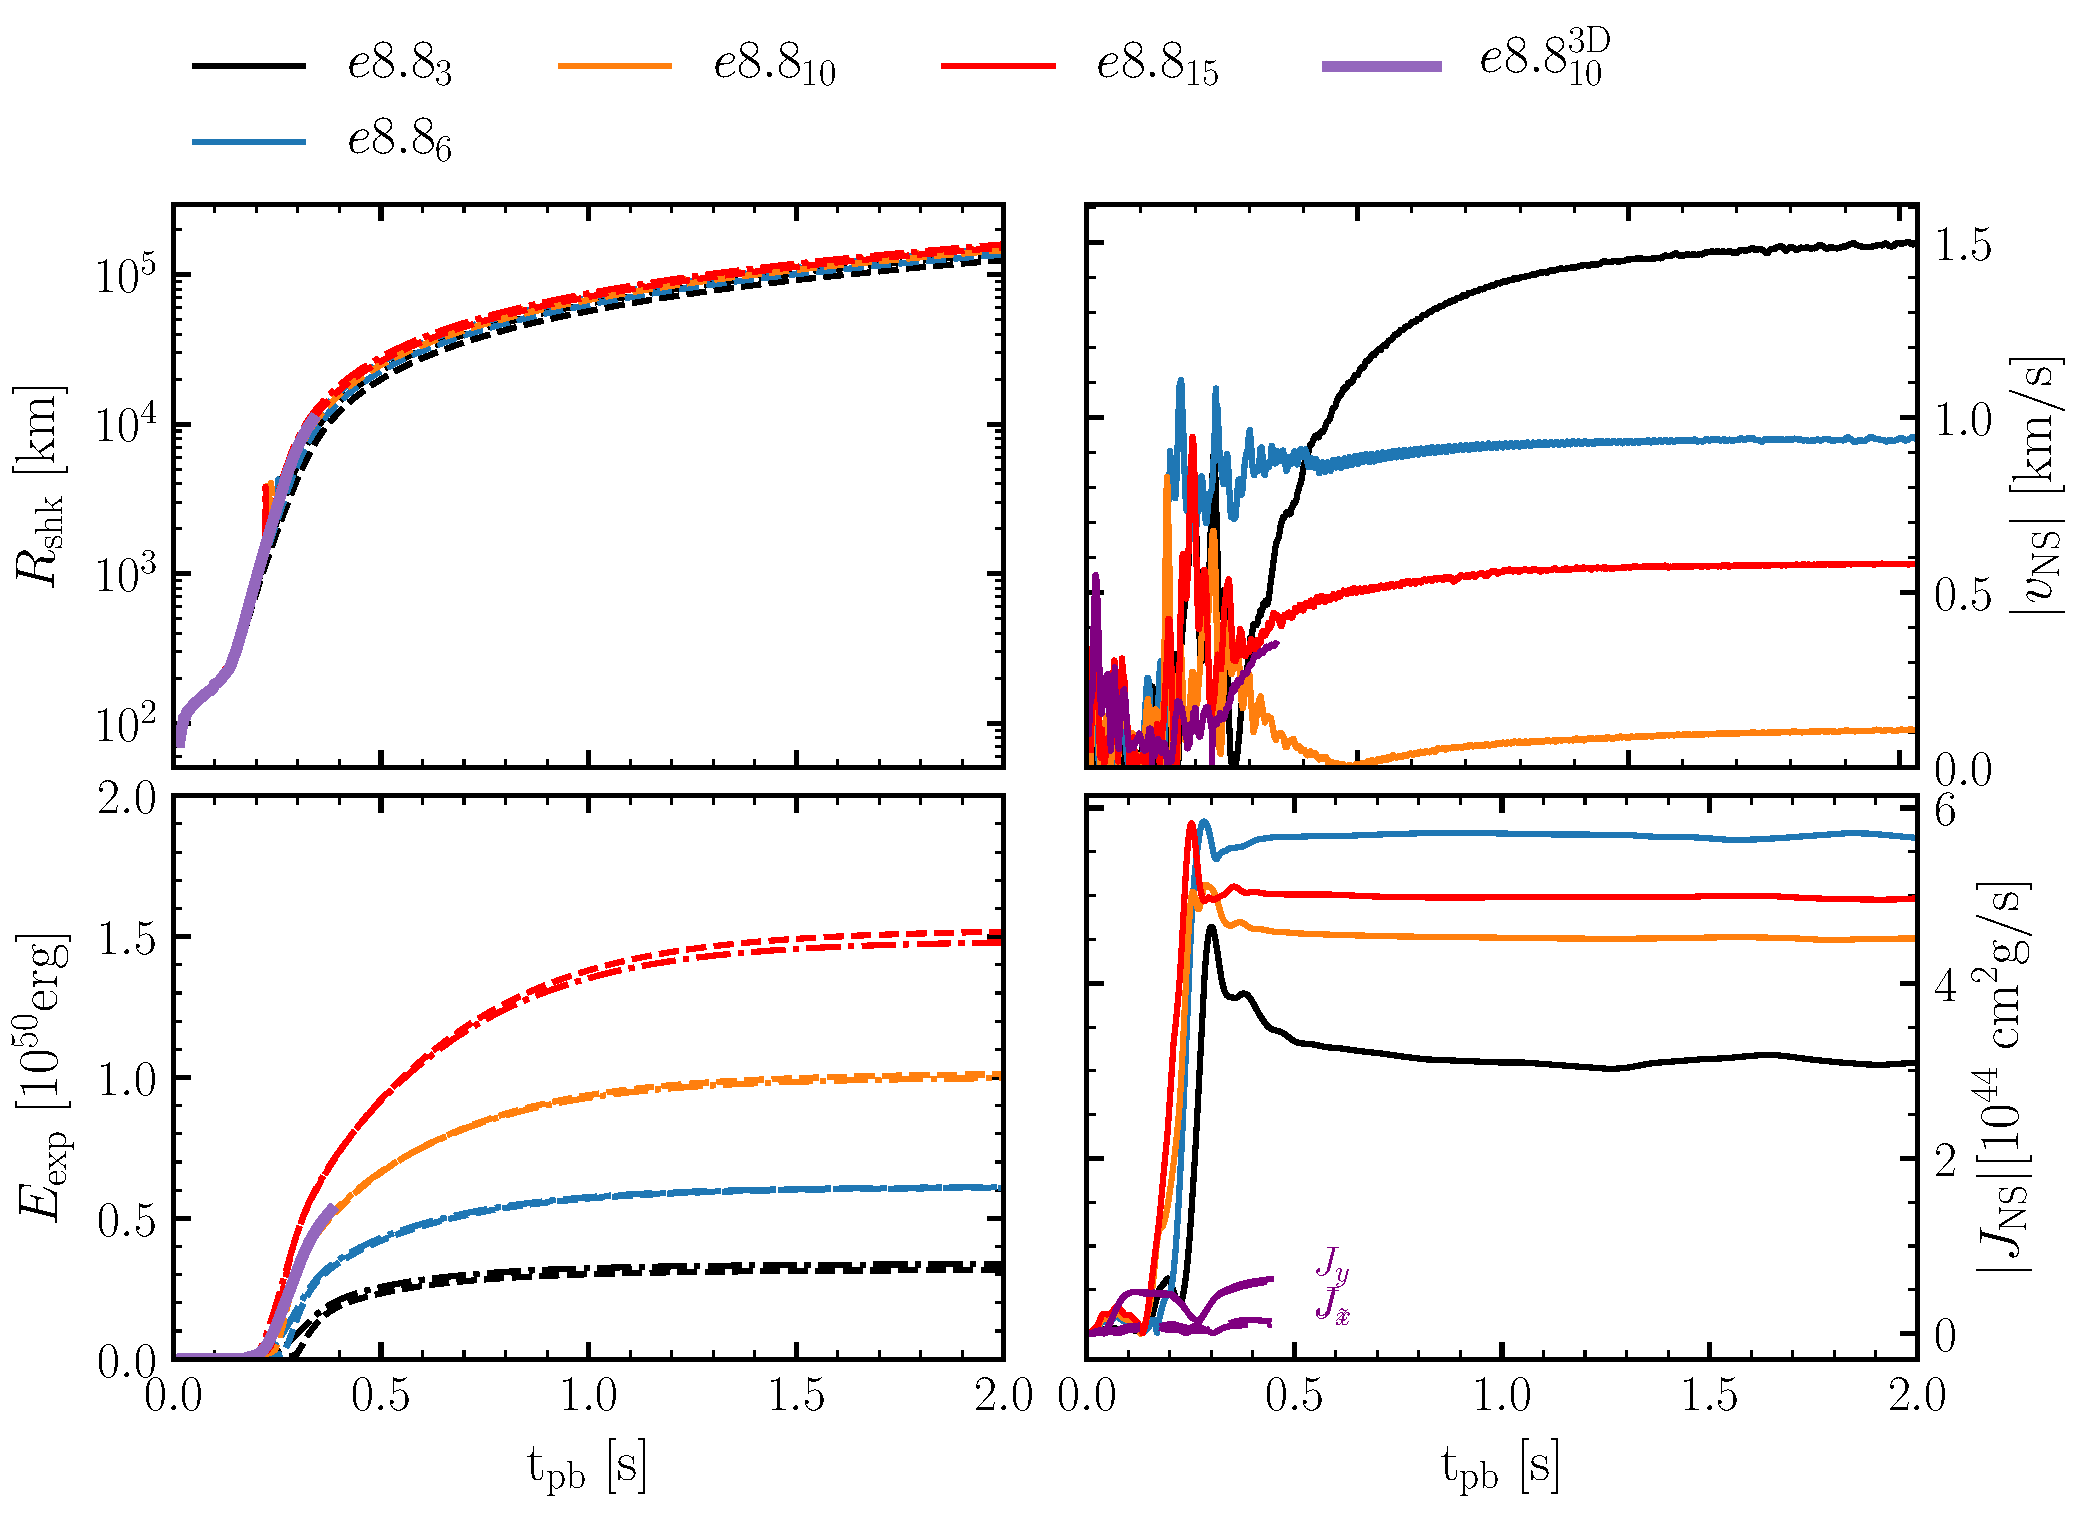
\includegraphics[width=0.79\textwidth]{pic/eexp_kick_all_1d2d3d.pdf}
 \caption{Various diagnostics for our electron capture models in all dimensions during the first 2 seconds post bounce. Upper Left: Shock radii. Upper right: Neutron star kicks. Lower Left: Explosion energies. Lower Right: Neutron star angular momentum. Note the very minor dependencies of the shock radii and explosion energies on dimension. }
\end{figure*}

In the upper right panel of \autoref{fig:e8pzkick} we show the neutron star kick velocities of all our calibrated models. In agreement with the simulations of \cite{Gessner2018} the terminal kick velocities are of the order of a few $\mathrm{km/s}$ only. AS been stated before explosions of ECSN progenitors do not develop large asymmetries in the ejecta which are needed for large neutron star kicks \cite{Scheck2006a}. Ascertaining this we add the evaluation of the asymmetry parameter to our analysis which is defined as 
\begin{equation}
    \alpha_{\mathrm{NS}} = \frac{|\mathbf{P}|_{\mathrm{gas}}}{P_{\mathrm{ej}}}
\end{equation}
where 
\begin{equation}
P_{\mathrm{ej}}=\int_{R_{\mathrm{NS}}}^{R_{\mathrm{shk}}}\rho |\mathbf{v}| \ud V
\end{equation}
and thus connects the net momentum of the gas with the scalar quantity $P_{\mathrm{ej}}$. Following the argumentation of \cite{Gessner2018} the asymmetry parameter that can vary between 0 for completely spherical explosions to 1 which would imply a fully one sided explosion, suits as a proxy describing the ejecta morphology. Results which are, among others, summarized in \autoref{tab:neutron star} reveal the small values of $\alpha_{\mathrm{ns}}$ for our ECSN model.
In addition we compute the neutron star spin by integrating the flux of angular momentum through a sphere of radius $r_{0}=500\;\mathrm{km}$ around the origin,
\begin{equation}
\label{equ:jns}
\frac{\mathrm{d}\mathbf{J}_{\mathrm{NS}}}{\mathrm{dt}} = \int r_0^2 \rho v_r \mathbf{v}\times \mathbf{r} \mathrm{d}\Omega
\end{equation}
In equation \ref{equ:jns} $\rho$ is the density, $\mathbf{v}$ and $\mathbf{r}$ are the vector valued velocity and position and $v_r$ the radial velocity. Considering the almost spherical explosion of our electron capture models only little transport of angular momentum onto the PNS is to be expected. This is evident in the lower right panel of \autoref{fig:e8pzkick} where we show the time evolution of the angular momentum of the produced neutron stars in our model set. Similar to the gravitational and hydrodynamical forces that cause the kick of the PNS transport of angular momentum onto the neutron star is strongest while the forward shock is still within the ONeMg core. After $300-350\;\mathrm{ms}$ the absolute values $\mathbf{J}$ are basically satiated.

In order to provide estimates for the spin period of the neutron star $P_{\mathrm{ns}}=I_{\mathrm{ns}}/|J_{\mathrm{ns}}|$, with $I_{\mathrm{ns}}$ being the moment of inertia of the PNS, we use the approximation by \citet{Lattimer2005} as given by
\begin{equation}
	I_{\mathrm{ns}} = 0.237M_{\mathrm{g}}R^2\Big[ 1 + 
    4.2 \Big( \frac{M_{\mathrm{g}} \mathrm{km }}{\solm R}\Big)  + 
    90 \Big( \frac{M_{\mathrm{g}} \mathrm{km }}{\solm R}\Big)^4
    \Big].
    \label{equ: ins}
\end{equation}
In the above equation $M_{\mathrm{g}}$ is the gravitational mass that can be estimated from the baryonic mass $M_{\mathrm{b}}$ to be (\citet{Lattimer2000})
\begin{equation}
	M_{\mathrm{g}} = M_{\mathrm{b}} - 0.084\Big( \frac{M_{\mathrm{b}}}{\solm}\Big)^2.
\end{equation}Spin periods and neutron star masses are, among other evaluations, summarized in \autoref{tab:neutron star}
Similar to what has been found by \citet{Muller2018b} there seems to be a anti-correlation between the spin periods and kick velocities. Higher $v_{\mathrm{ns}}$ produce slower rotating neutron stars.

\begin{table*}
\centering
\begin{tabular}{ccccccccc}
            & $v_{\mathrm{NS}}$& $J_{\mathrm{NS}}$    & $\alpha_{\mathrm{ej}}$& $M_{\mathrm{b}}$& $M_{\mathrm{g}}$ & $P_{\mathrm{NS}}$& \rns \\
    Model & [km/s]           & $[10^{44}\; \mathrm{cm^2 g/s}]$ &         [\%]              &  [\solm]        &  [\solm]         & [s]              &  [km] \\
    
    \hline 
    $e_{3}$  &      1.55316 &             2.40843 &   1.154 &     1.32267 &      1.17572 &  57.18667 &  49.85177 \\
    $e_{6}$  &      0.93943 &             4.85824 &   0.0408 &     1.31627 &      1.17073 &  28.65161 &  50.22289 \\
    $e_{10}$ &      0.12700 &             4.47504 &   0.0036 &     1.30839 &      1.16459 &  31.37448 &  50.57279 \\
    $e_{15}$ &      0.59041 &             4.93726 &   0.0116 &     1.29937 &      1.15755 &  28.58571 &  50.85872
\end{tabular}
\caption{Notes: The columns are from left to right, terminal kick velocity, angular momentum, anisotropy parameter, baryonic neutron star mass, gravitating mass, estimated spin period and neutron star radius.}
\label{tab:neutron star}
\end{table*}

\subsection{Explosion Dynamics of the z9.6 Model}
Since the first second after bounce is described in depth by \ref{Melson2015} we summarize the evolution here. 
Due to the relatively steep density gradient just outside the iron core the forward shock begins to expand rapidly already at around 300 ms post bounce even in 1D. The explosion energy however remains small at $\mathrm{E_{exp}}=(0.17-0.28)\times 10^{50} \; \mathrm{erg}$ and the explosion sets in at late times of $\mathrm{t_{pb}}\approx 300\;\mathrm{ms}$. As stated in \cite{Melson2015} multidimensional effects, missing in the 1D simulation, are the necessary ingredient for higher explosion energies. The spherical symmetric simulation however still can teach us about the global evolution of the multi-D runs as will be shown in Section \ref{subsec:instabilities_prior}.
In 3D shock expansion is aided by convective overturn that starts to develop at $t_{\mathrm{pb}} > 70\;\mathrm{ms} $ and reaches its maximum at around $t_{\mathrm{pb}} \approx 200\;\mathrm{ms}$ 200. This turbulent motion triggers shock acceleration to velocities up to $\mathrm{250.000\;km s^{-1}}$ while the ejecta remain nearly self-similar in their structure. 
At the time when the \vertex simulation stops radial velocities in the post shock region only show maximal absolute deviations from the background of about 50\%\footnote{Deviations from the background are calculated via $\delta v_r = | (v_r - \langle v_r \rangle>_{\Omega}) / v_r |$}. This is in stark contrast to the $s9.0$ model presented in the next section. 


\subsection{Explosion Dynamics of the s9.0 Model}
\textcolor{red}{\textbf{More INformation needed}}
In contrast to the $z9.6$ model this iron-core progenitor does not explode self-consistently in 1D. As can be seen in Figure \ref{fig:rho_rcubed_interfaces} the solar metallicity star is lacking the very steep density gradient outside the Fe-core present in the other 2 models. The shock can expand initially up to 140 km at $t=100$ [ms] p.b. but then declines as accretion overpowers the neutrino heating below the shock radius. 
Multidimensional effects however enable a successful explosion in 3D.  Due to the fairly steep density gradient outside the iron core ( compared to more massive models at around 20\solm) the resulting low mass accretion rate produces large advection time scales and thus favorable conditions for convection to grow. Note that the gain layer, the region where neutrino heating is stronger than neutrino cooling confined by the shock radius,  is too large to support the growth of a pronounced SASI (standing accretion shock instability) mode, since a greater extend of the standing shock radius suppresses SASI. Although no SASI develops, the shock shows a dipolar deformation of around 6\% in comparison to its angle averaged value. Larger scale plumes that formed during the explosion merged and pushed the forward shock outward in one hemisphere. 
% LESA ??
% Velocities 
\textcolor{red}{\textbf{Lesa ? Kick ?}}
\textcolor{red}{\textbf{Plots of velocity/mass distribution}}
\textcolor{red}{\textbf{Plots of column densities}}

\subsection{Morphology of the ejecta after shock revival}
\label{subsec:Morphology of the ejecta after shock revival}

As has been shown by \cite{Kifonidis2003} the density perturbations set by convective overturn during the explosion phase are a key ingredient for subsequent growth of the Rayleigh-Taylor instability. \cite{Kifonidis2003}  noticed that if these perturbations are small RT fingers grow, as predicted by theory (\cite{Chandrasekhar1961}), also on small scales and are thus not able to accelerate metals to the high velocities, which are needed for example to explain the high \nickel velocities found in observations of SN1987A. In a subsequent study with a similar progenitor but different numerical setup the time of explosion was delayed by several 100 ms. This led to larger high-entropy plumes that deformed the forward-shock considerably with an l $\sim$ 2 mode. These plumes provided the ground for the needed high velocity tail of the ejecta. This is in line with the results of \citet{Wongwathanarat2015} that find a correlation between the largest initial plumes and fastest nickel rich shrapnels at the end of their simulation. It is thus important to understand the physical state of the models when the shock is revived and begins to propagate through the envelope of the star.

% e8.8 
In the case of the electron capture models the fast shock expansion and early explosion lead to an almost perfectly spherical shock. Additionally density and pressure perturbations within the post shock material are small in amplitude with only a few over-dense regions at the heads of the convective plumes. 
This suggests that RTi unstable layers may develop many small scale plumes as the Rayleigh-Taylor instability grows faster for higher wave-number (\cite{Guilet2009}) and also observed for a model with a short explosion timescale in \cite{Kifonidis2003}.
The sphericity of the explosion is also reflected in the distribution of the elements over mass and velocity space as shown in the right panels of \autoref{fig:mdp_first_mapping}. The initial shell structure of the progenitor is still visible in velocity space with additional low velocity helium and carbon that was produced from the seeds of NSE freeze-out and subsequent burning. Same holds true for the mass distribution. 

%z9.6
As convection was somewhat more violent in $z9.6$ model as in the $e8.8$ models mixing in mass and velocity space was more efficient. Although the initial structure of the progenitor is still imprinted on the distribution (the bulk of carbon and oxygen travels ahead of the iron group nuclei), the separation is not that extreme as in the electron capture model. The post shock density distribution is broader and density perturbations in the post shock material are larger in amplitude than in the electron capture case. Most important however the deceleration of the forward shock at the Si/O and CO/He interfaces already compressed some of the matter into a dense shell. This has important consequences as detailed in \autoref{subsec:muldidimensional longterm z9}.
Note that the hydrogen displayed in the left two panels of \autoref{fig:mdp_first_mapping} is left over by the freeze-out of NSE and not hydrogen from the envelope. 

%s9.0 
The ejecta morphology of the  $s9.0$ model is in strong contrast to both models described above. This is caused by various reasons. 
The core structure of the solar metallicity star is minted by several clearly separated interfaces imprinted in the $rho r^3$ profile. Passing of the forward shock through one of these interfaces feeds the instabilities caused by neutrino heating in the gain region.
Additionally a more massive helium core leads to larger accretion rates hampering shock expansion and prolonging the time for convection to grow.

The initial onion shell structure of the progenitor is thus completely erased and elements are homogenously mixed over mass and velocity (see middle panels of \autoref{fig:mdp_first_mapping}).
The strong convection also leads to a fairly asymmetric shock expansion at $t_{\mathrm{pb}}=0.4\;\mathrm{s}$ that is driven by a large high entropy plume accompanied by large downflows in the opposite hemisphere. 

%% FIGURE Mass Distribution all Progenitors
\begin{figure*}
 \centering
 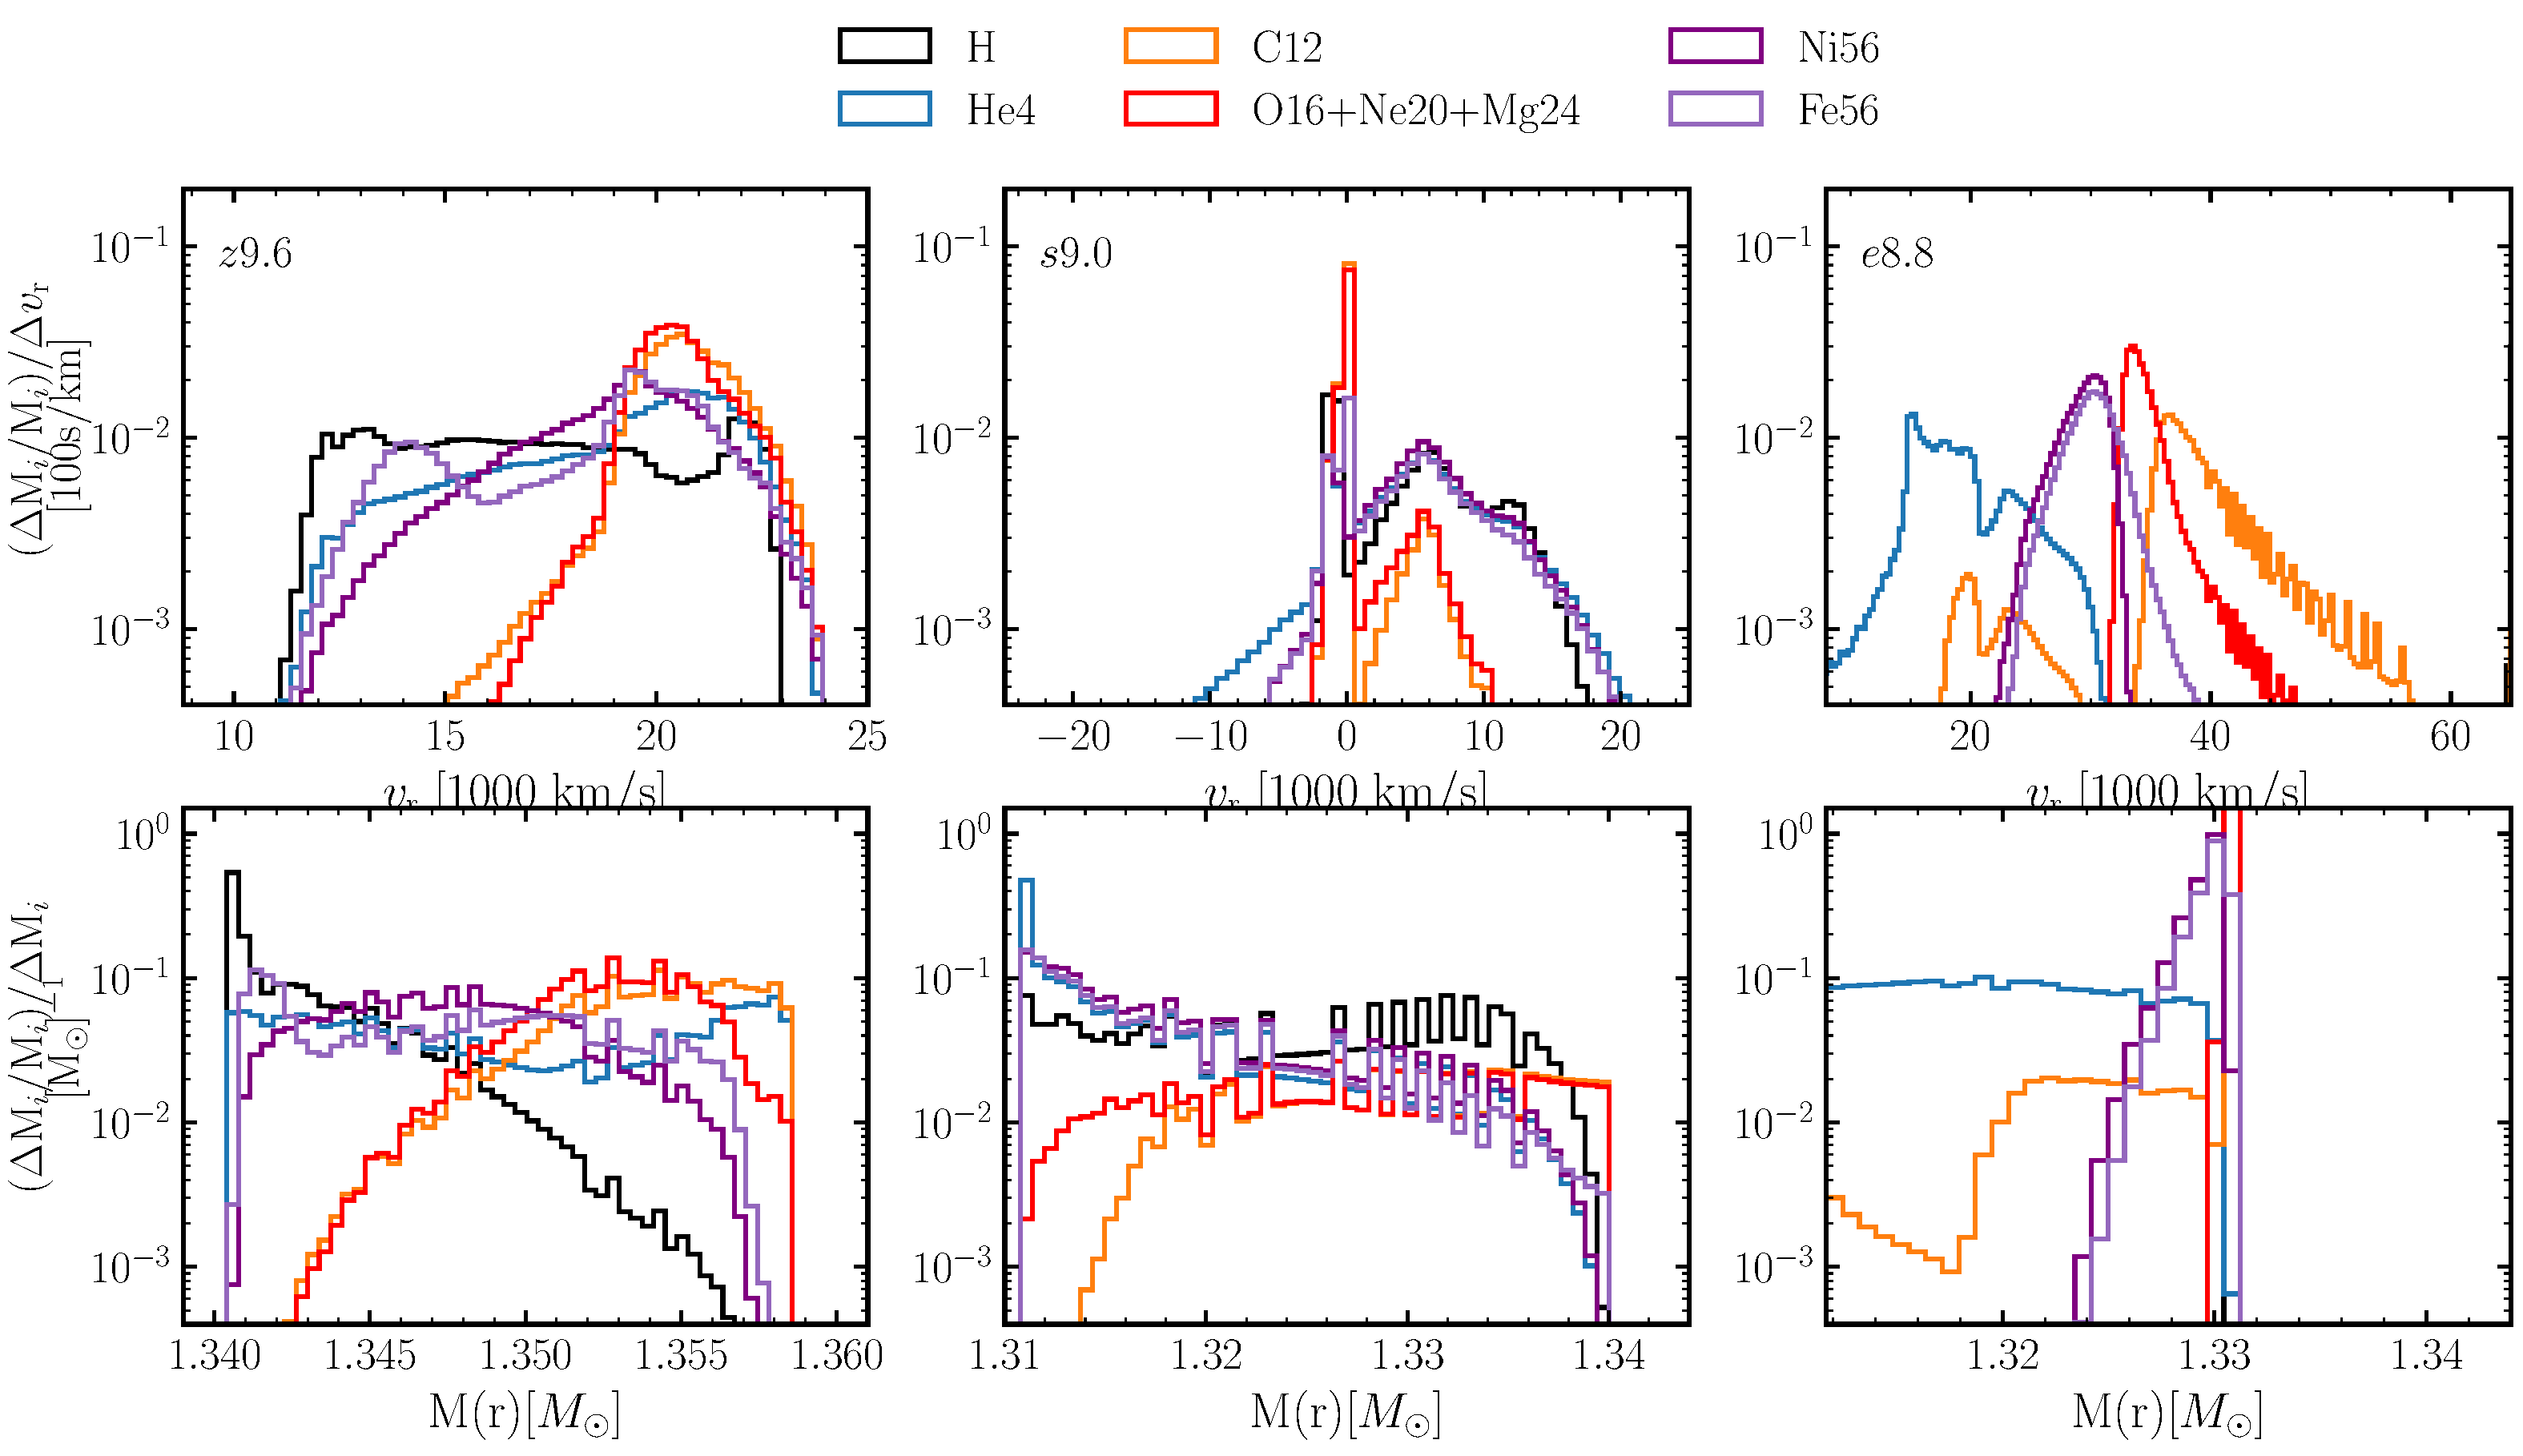
\includegraphics[width=0.9\textwidth]{pic/z96_s9_e8_massDis_mvr_and_masstime_0.pdf}
 \caption{Mass distribution in mass and velocity space for all our models after we excised the inner parts from our simulations. The exact post bounce times are $0.425 \;\mathrm{s}$ for the $e8.8_{10}$, $1.466 \;\mathrm{s}$ for the $z9.6$ and $1.054 \;\mathrm{s}$ for the $s9.0$ }
 \label{fig:mdp_first_mapping}
\end{figure*}

\section{Evolution to shock-breakout}
In order to anticipate the global behaviour of the 3D long-term simulations we conducted 1D simulations with the same initial setup. Of special interest is the propagation of the forward shock, the points in time when it passes composition-interfaces, when and how the reverse shock forms and falls back onto the PNS.

For the ECSNe progenitor the one-dimensional calibration runs where continued starting from $t_{\mathrm{pb}} = 2.515 \;\mathrm{s}$ whereas the 1D runs of the iron-core progenitors were started from angle averaged states of the 3D data sets. 
As has been stated before special care was taken to only excise bound matter that resides within $R_{\mathrm{sonic}}$
to ensure that no transients caused by the cutting procedure can move into the ejecta.

In the following we firstly present the behaviour of our one dimensional simulations and estimate the occurrence and strength of possible hydrodynamical instabilities before analyzing the results of our 3D simulations.

\subsection{Spherical symmetric simulations}
\subsubsection{Long term evolution of the $e8.8$ model}

When we continue the simulation of the $e8.8$ model starting from $t_{\mathrm{pb}}=2.515\;\mathrm{s}$ the forward shock has long passed the He/H interface and is traveling through the H-envelope. The forward shock left the ONeMg core with some $7.5\times 10^{9}\mathrm{cm/s}$ which now travels at $5.8\times 10^{9}\mathrm{cm/s}$. The early and strong deceleration of the forward shock at the edge of the ONeMg core at $t_{\mathrm{pb}}=0.17\;\mathrm{s}$ has formed a high density shell, bounded by a reverse shock at its inner shoulder, separating the post shock material from the innermost ejecta.  
This has important consequences for the overall evolution of the model as well as for the growth of Rayleigh-Taylor instabilities and achievable velocities for the neutrino heated ejecta which will be discussed later on.
Over the following hours the forward shock closely follows the analytic prescription of \citet{Matzner1998}, decelerating as it increases total ejecta mass\footnote{According to \citet{Matzner1998} the shock velocity can be calculated as $\mathrm{v_{sh}=0.794\times(\frac{E_{exp}}{M_{ej}})^{1/2}(\frac{M_{ej}}{\rho r^3})^{0.19}}$, where $\mathrm{E_{exp}}$ is the explosion energy and $\mathrm{M_{ej}}$ is the unbound matter.}. Due to the increase in ejecta mass and the continuous deceleration of matter behind the shock  the reverse shock begins to travel back in mass at  $t_{\mathrm{pb}}\sim 1\;\mathrm{h}$. It takes however additional $7\;\mathrm{h}$ for the reverse shock to reach the inner boundary of our computational domain $(t_{\mathrm{revsh,ib}}=t_{\mathrm{pb}}\sim \; 8\;\mathrm{h})$. The passing of the reverse shock and its reflection at the inner boundary flattens the inner density structure to a constant profile of $\rho\approx 10^{-8}\;\mathrm{g/cm^3}$.
As the forward shock travels unaffected by the processes in the interior through the hydrogen envelope it converts almost 50\% of its kinetic energy into heating the hydrogen gas, thus further decelerating. Due to this and the huge size of the envelope ($R_{*}\approx8.8\times10^{13}\;\mathrm{cm}$) shock breakout occurs around 3 days in the highest energy case and just over 5 days in the lowest energy case after shock left the ONeMg core. At this time the shock travels with about $v_{\mathrm{sh}}\approx 5\times 10^{7}\; \mathrm{cm/s}$ accelerating to some $2.6\times 10^{8}\; \mathrm{cm/s}$ as it leaves the star.

\begin{table}
%\centering
   \begin{tabular}{l| l | l }
  \label{table:e8Fallback}
  Name & 1D & 2D \\
  \hline \hline
  $\mathrm{e}8.8_{3}$ & 2.446 	&	 2.51  \\
  $\mathrm{e}8.8_{6}$ & 1.582 	& 	1.667  \\
  $\mathrm{e}8.8_{10}$ & 0.928	& 	0.662  \\
  $\mathrm{e}8.8_{15}$ & 0.245 & 	 0.251 \\
  \end{tabular}
\caption{Total Fallback of the electron capture simulations in $\mathrm{10^{-4}\;M_{\odot}}$ measured at the inner boundary. }
\end{table}

\subsubsection{Long term evolution of the $z9.6$ model}
\label{subsec:z96 1d}
% z9.6 1D
The one dimensional run of the $z9.6$ is started from spherically averaged values of the respective 3D model\footnote{The recombination of remnant neutrons and protons of the \vertex simulation lead to a very small transient that does not change the evolution of the model.}. At this time the the forward shock $(R_{\mathrm{s}}(t_0) = 3.84\times 10^4 \mathrm{km})$ just passed the former C/He interface beginning its journey through the He core.

During the first 10 seconds of our simulation the evolution of the ejecta is dominated by the injected neutrino driven wind. The accelerated material encounters the post-shock matter with supersonic velocities creating the so-called wind-termination-shock (see e.g. \citet{Arcones2006}). \citet{Arcones2006} also noted that the increase in entropy and temperature at the termination shock can influence the nucleosynthesis. In the $z9.6$ case however matter has expanded to  $R_{\mathrm{term shk}} \geq 10^{9}\mathrm{cm}$ where temperatures and densities are too low and nuclear burning has ceased. 
As the PNS cools and neutrino reactions in its atmosphere, and thus energy and pressure causing the wind, subside. Consequently the wind-termination shock weakens and thus falls back in mass coordinate until it leaves the grid at our inner boundary at $t_{\mathrm{pb}}\sim 12\;\mathrm{s}$. Although fallback velocities are fairly large only very little matter ($\mathrm{M_{fb}}(t=12\;\mathrm{s})=8.71\times 10^{-5}\mathrm{M_{\odot}}$) falls back onto the PNS. Note that the strength of the neutrino driven wind, that is almost non-existent in the ECSNe case, sets the maximum velocity the iron rich material can achieve and prevents strong deceleration of the forward shock in the envelope (\citet{Wongwathanarat2015}). 
Similar to the evolution of the forward shock in the hydrogen layer of the ECSN progenitor, continuous deceleration of the forward shock in the He layer causes the formation of a reverse shock fairly early at some $t_mathrm{pb}\approx 10\;\mathrm{s}$. Until $t_{\mathrm{pb}}\approx \; 300\;\mathrm{s}$ forward and reverse shock travel with similar speed through the He core where $\mathrm{R_{rev.shk}\approx 0.72\;\times R_{shk}}$. 
Again the shocks clearly separate two different regimes in the ejecta. The inner neutrino heated ejecta bounded by the thin dense shell at the reverse shock and the lower density material between the shocks in which $\partial v_{\mathrm{cs}}/\partial r > 0$. This, in mass coordinate small region, is prone to the RTi. %
At later times ($t_{\mathrm{pb}} > 300  \mathrm{s}$) this ratio decreases until the reverse shock reaches the inner boundary at $t_{\mathrm{pb}}\sim 4100\;\mathrm{s}$, so more than 4 hours earlier than in the $e8.8$ case. The passing of the reverse shock compresses the inner ejecta leaving behind a low density bubble rather than a constant density profile as found in the electron-capture case.
The interaction of the reflected reverse shock with the ejecta is also more dynamic as in the ECSN case. Non-linear waves travel back and forth bounded by the inner boundary and inner shoulder of the high density shell created while passing the He core. Eventually two high density bumps remain where at the time of shock breakout $(t_{\mathrm{bo,pb}}\approx\; 29\mathrm{h})$ the immediate post shock material is followed by the inner bump located close to the former He/H interface. %
As the gradient of the $\rho r^3$ profile does not change considerably across the He/H interface the evolution of the inner high density region is not affected by additional reverse shocks and remains within the former He/H interface at $R_{\mathrm{He/H}}\approx 1.5\times 10^{12}\; \mathrm{cm}$ until $t_{\mathrm{pb}}\sim 35.5\;\mathrm{h}$.

After shock breakout the forward shock expands into the ambient medium which is heated and accelerated. In turn the material pushes back into the ejecta (see \citet{Truelove1999}) creating a reverse shock since the expansion happens faster than the local sound speed. The density and velocity profile approaches the simplified picture presented in \citet{Truelove1999} where  $\rho \sim r^{-14}$ up to $r=R_{\mathrm{shk}}$. 
The innermost structure is only changed when the heat produced by the $\beta$ decay of \nickel causes matter to expand and thus compresses some of the material above into a dense shell at $M(r)\approx 1.36\; \mathrm{M_{\odot}}$. Changes in the velocity of the inner material are minor however due to the little amount of \nickel produced.

\subsubsection{Long term evolution of the $s9.0$ model}
Given that the $s9.0$ model is fairly asymmetric compared to the zero metallicity progenitor or the electron capture model, the angle averaged model for the 1D simulation shows a smoothed out density and velocity profile and thus a smoothed out shock. Thus results from this simulation are even more qualitative than for the other two cases.
When the forward shock leaves the CO-core it accelerates to its maximum value of $0.8\times 10^{9}\mathrm{cm/s}$ . As it travels through the He4 shell it is decelerated piling up matter in a dense shell behind it. When it reaches the H/He4 interface ($\sim 200$ [s]) the drop in density sends a pressure wave back into the ejecta that steepens into a reverse shock. Note that this reverse shock begins to fall back relatively late at around 22 [h] and reaches the inner boundary as late as 37 [h]. The reflected shock wave runs back into the ejecta while at 90 [h] the forward shock breaches the surface of the star. Due to this the density structure looks quite different to the $z9.6$ model. The large cavity is less pronounced and confined by a dense shell at its lower boundary. 

\subsection{Linear Stability Analysis}
\label{subsubsec:Linear Stability Analysis}
According to Sedov \cite{Sedov1961} a change in the shock velocity can be expected where the density gradient is smaller/\NY{grater}{ greater} than $r^{-3}$. This acceleration and deceleration produces a density/pressure inversion in the post-shock regime making it unstable to the Rayleigh-Taylor instability. As the $\rho r^3 $-profiles vary strongly between the different progenitors the respective estimates for the growth of the RTI differs in amount and position in mass coordinate.
To have a quantitative estimate of the dynamical evolution of the ejecta we computed the linear Rayleigh-Taylor growth rates from our 1D simulations. A fluid is prone to the RTi if radial density- and pressure-gradients have opposite signs, or stated otherwise, the sound speed of the material increases with radius. Following \cite{Mueller1991} we calculate the growth rate of \NY{some}{} initial \NY{perturbation}{ perturbations} as
\begin{equation}
  \label{equ:growth_rates_incmp}
  \sigma_{\mathrm{RT,incmp}} = \sqrt{- \frac{p}{\rho}\frac{\partial \ln p}{\partial r}\frac{\partial \ln \rho}{\partial r}}
\end{equation}
in the incompressible case and
\begin{equation}
  \sigma_{\mathrm{RT, cmp}} = \frac{c_{s}}{\gamma}\sqrt{\Big(\frac{\ln p}{\partial r}\Big)^ 2 - \gamma \frac{\partial \ln p}{\partial r}\frac{\partial \ln \rho}{\partial r}}\label{equ:growth_rates_cmp}
\end{equation}
in the compressible case, where $c_s$ is the local speed of sound. Note that \autoref{equ:growth_rates_cmp} is less restrictive than its incompressible counterpart\footnote{Note that we are interested in the position of maximal growth not in the actual value. Calculating the growth rate from multidimensional models using angle averaged values gives similar overall structure but lower amplitudes.}. 
For the final growth at a certain point in time we integrate \autoref{equ:growth_rates_cmp} according to

\begin{equation}
  \Sigma_{\rm RT}(t) = \frac{\xi}{\xi_0}(t) = \exp \left(\int_0^t \sigma_{RT} (t') dt' \right),\label{equ:growth_rates_int}
\end{equation}
giving a lower bound for the actual growth rate. This analysis enables us to estimate the time and location in mass coordinate when the fluid becomes unstable to the RTi and helps us to understand the origin of possible fast moving clumps of material.

The estimated growth rates for all models are summarized in \autoref{fig:growth_rates}, where large differences between the models are evident. Note that we use the $e8.8_{10}$ model as our reference for the evaluation of $\Sigma_{\mathrm{RT}}$.


\begin{figure}
 
 \centering
 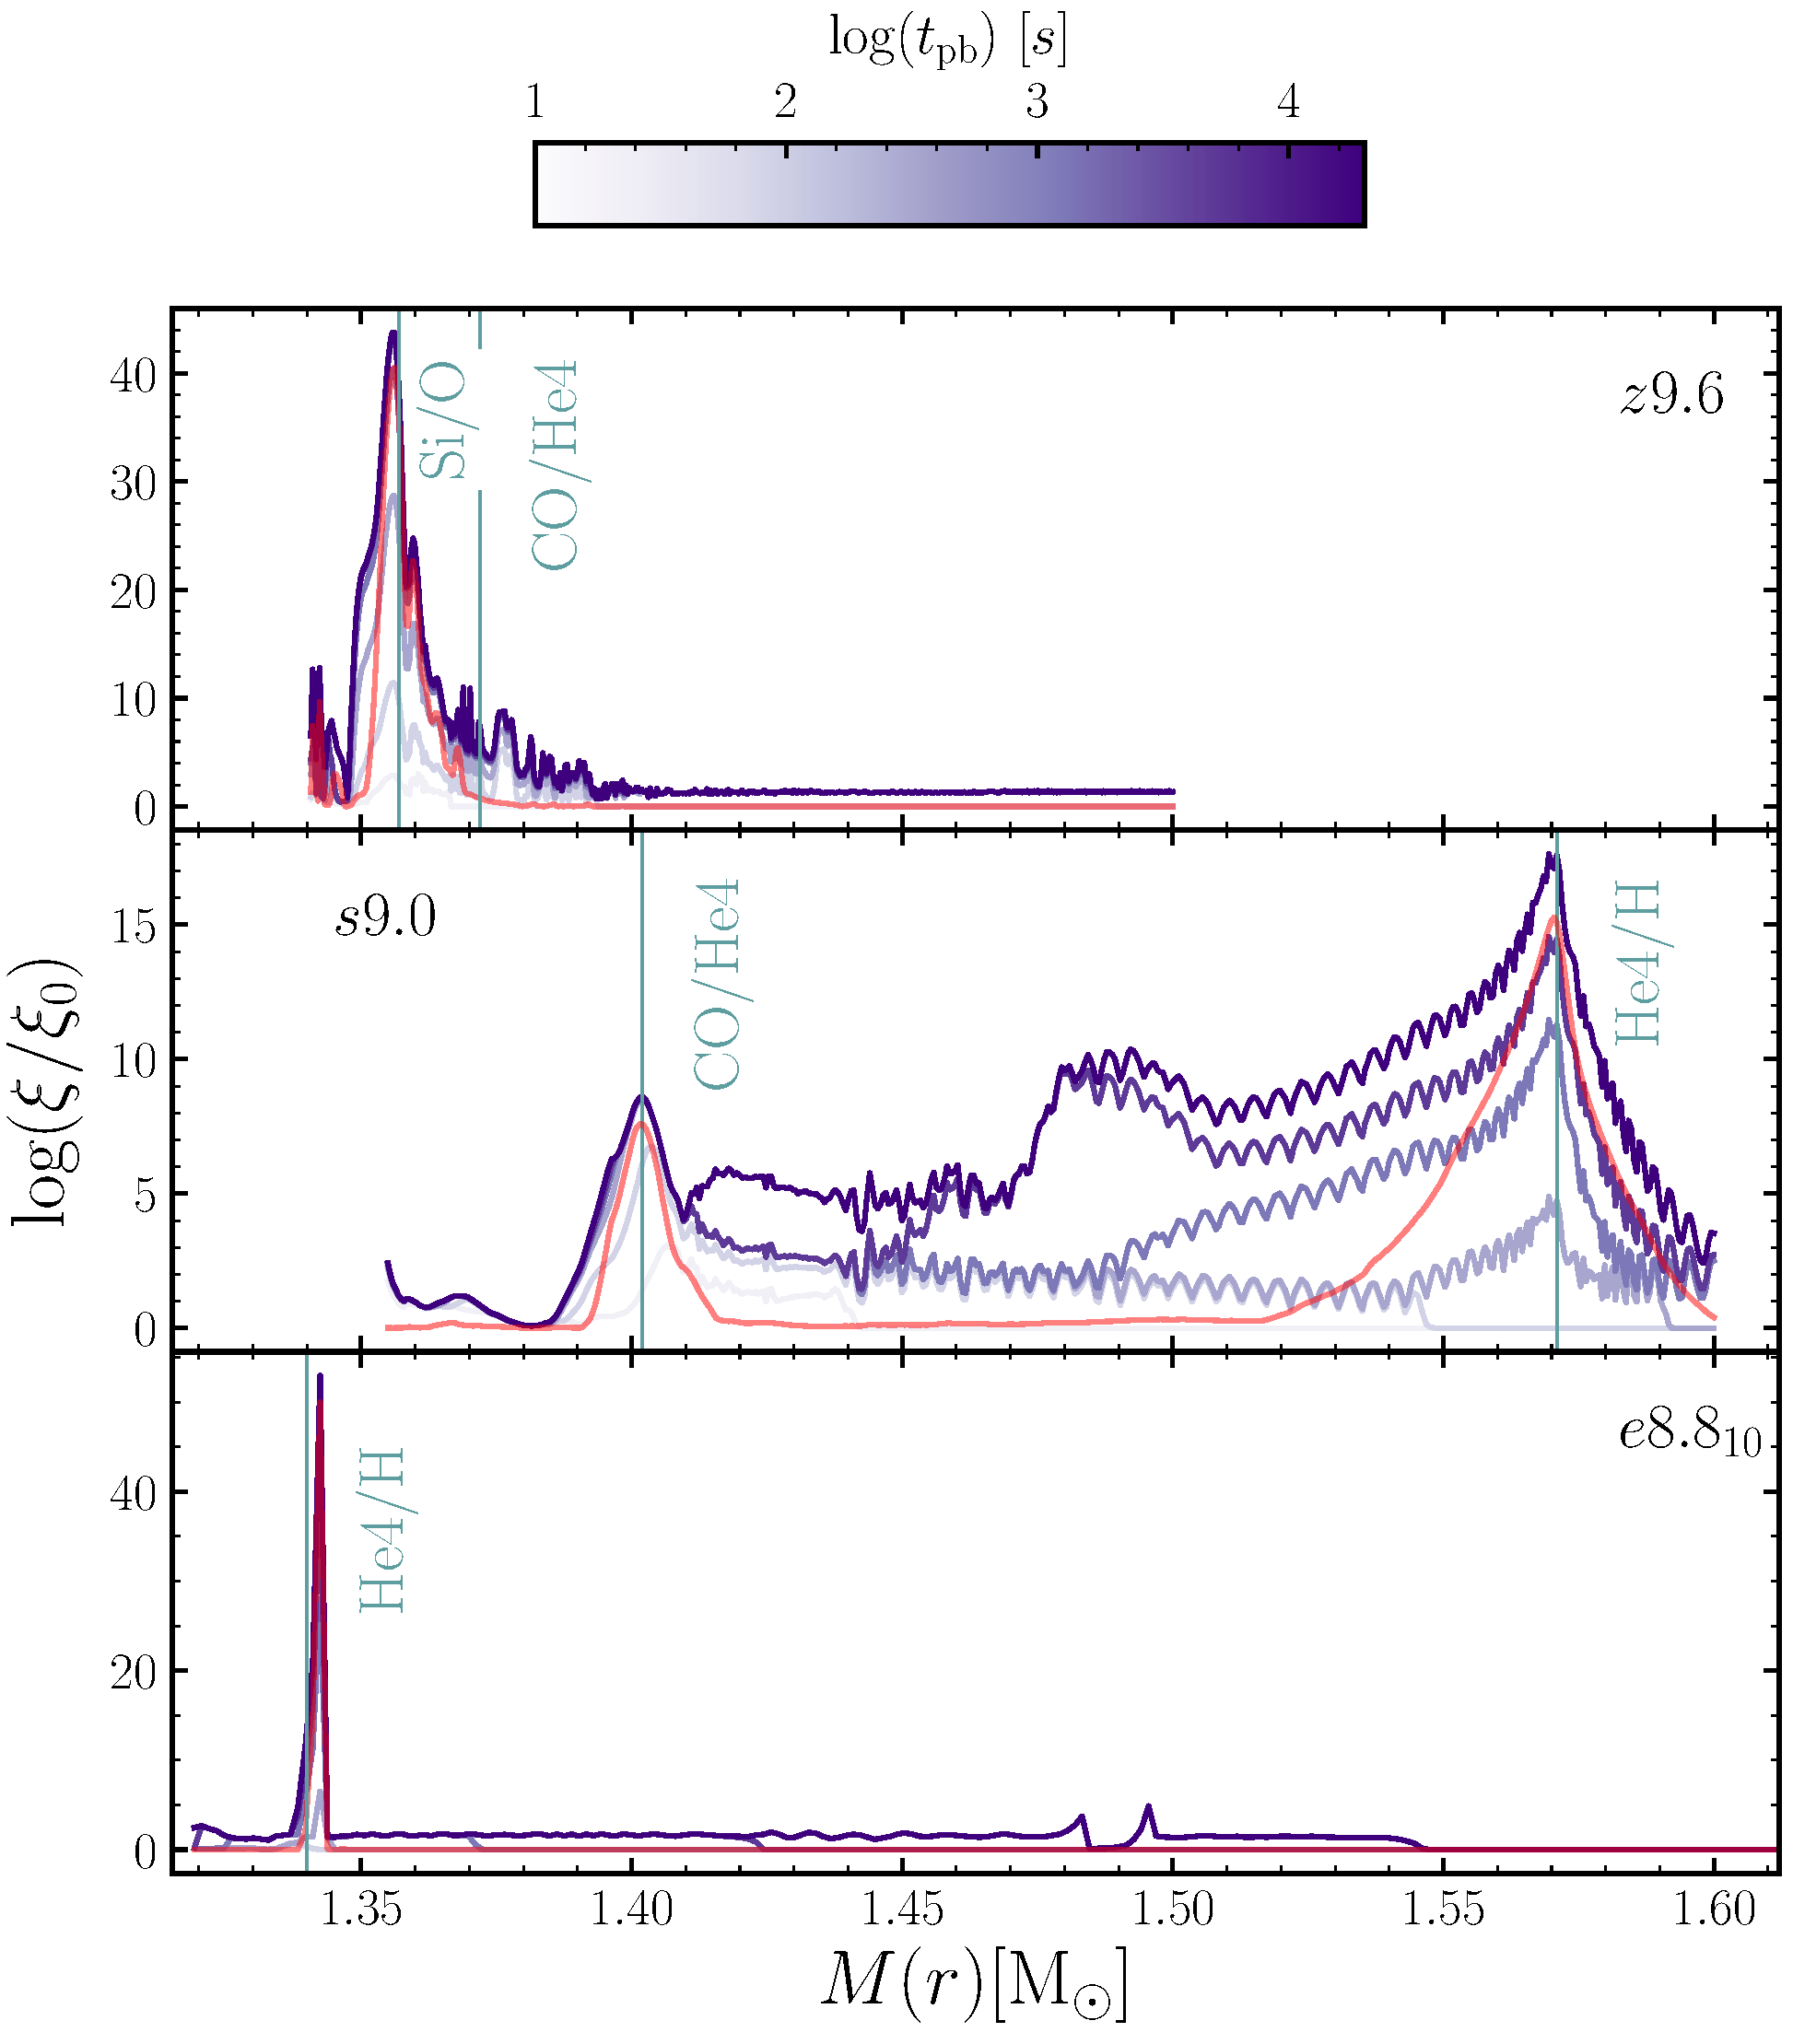
\includegraphics[width=0.49\textwidth]{pic/growth_rates_1d.pdf}
 \caption{Integrated growth rates for all considered models at different times according to \autoref{formula:growth_rates_int}. Indicated by the blue lines are the respective composition interfaces. The red line denotes the evaluation of the growth rates in the incompressible limit at $t=10^{4}\;\mathrm{s}$. The different progenitor structures have a large impact on the estimated growth as can be seen most prominently by comparing the z9.6 and so s9.0 models. }
 \label{fig:growth_rates}
\end{figure}

The extreme deceleration of the forward shock, and the resulting inversion of the pressure gradient, outside of the core of the ECSN leads to very high growth rates at $M(r)=1.34\;\mathrm{M_{\odot}}$ as it is visible in \autoref{fig:growth_rates}. However early formation of the reverse shock confines the RTi unstable layer within a tiny mass shell. Consequently no strong mixing of  neutrino heated material into the envelope is expected.

The iron core progenitor with most similar structure to the electron capture progenitor is the $z9.6$ which is reflected in the growth factors as well.
The fairly steep density gradient outside the iron core flattens abruptly at the Si/O interface however. Consequently shock deceleration at the passage of the interface sends a pressure wave in the ejecta creating the necessary ingredients for the RTi to grow. As can be seen in \autoref{fig:growth_rates} terminal growth rates at this interface almost reach values as high as observed in the ECSN case. The CO/He interface contributes only little to the overall strength of the RTi and is barley visible when the incompressible approximation is used.

The $s9.0$ shows striking differences to the models described above. 
Due to its more shallow $\rho r^3$ profile and the consequently weaker episodes of de- and acceleration, the peak amplitudes of the growth factors are smaller. They are however in the ballpark of the models investigated by \citet{Wongwathanarat2015}. 
Similar to the RSG-models presented in \citet{Wongwathanarat2015} the strongest contribution arises from the He/H interface followed by the CO/He interface reaching amplification factors of $8-16$ respectively. 
A feature not observed in the previously described models is the vast difference in the compressible versus incompressible evaluation of the growth factors. In the compressible case a large contribution between both interfaces is visible, suggesting additional mixing at some $t_{\mathrm{pb}}\approx 1\times 10^{(3-4)}\;\mathrm{s}$. This is enabled by the propagation of the reverse shock through the ejecta that is not captured in the incompressible case. 

\begin{figure*}
 \centering
 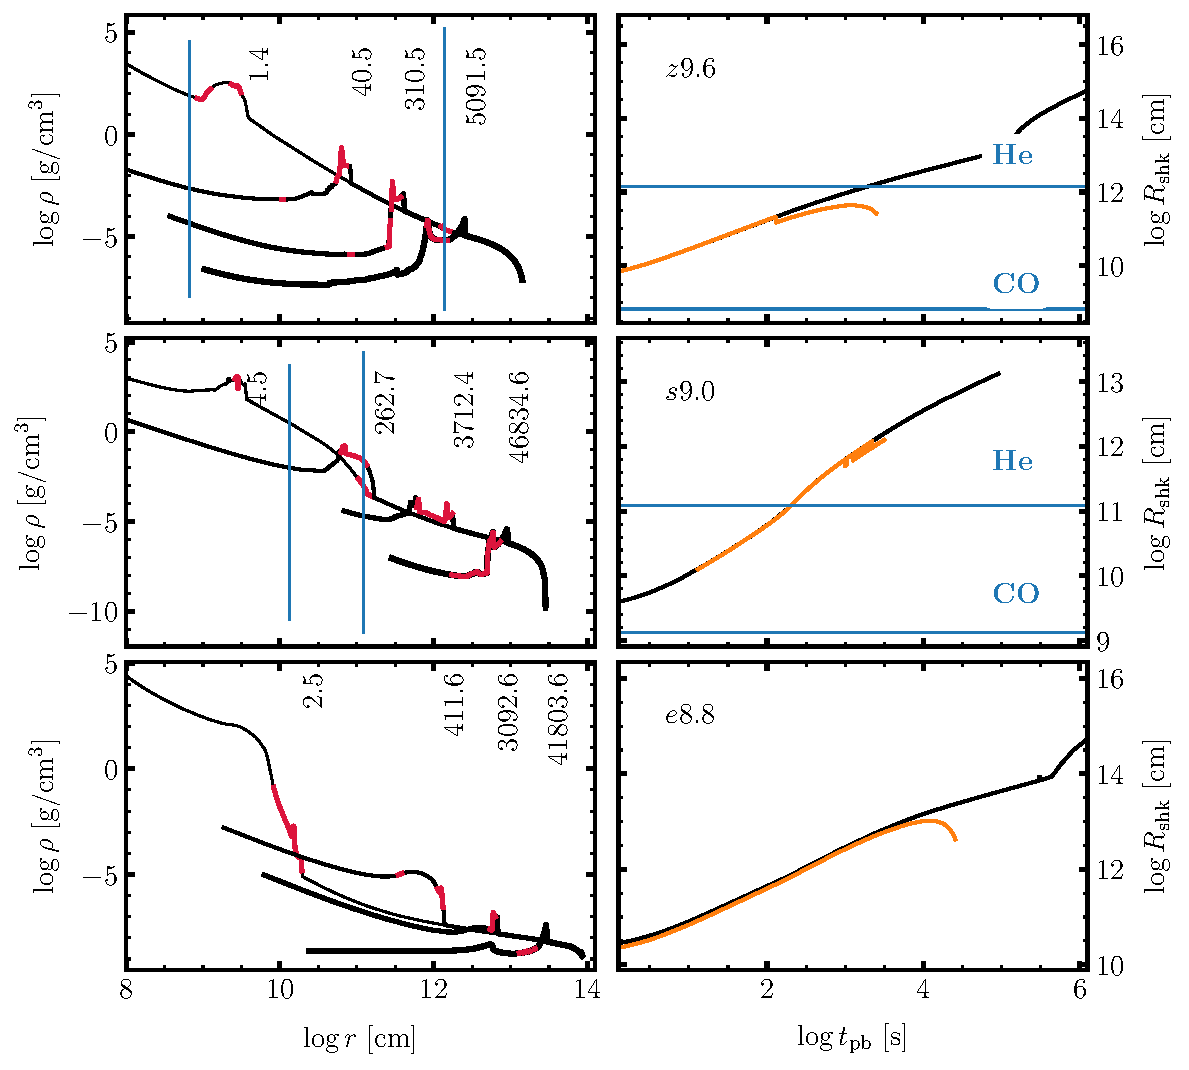
\includegraphics[width=0.8\textwidth]{pic/density_times_all.pdf}
 \caption{Left Panels: Snapshots of the density distribution of the $z9.6$, $s9.0$ and $e8.8$ models. Marked in Blue are regions of positive $v_{\mathrm{cs}}$ gradient and thus RT unstable region. Note the early formation of a dense wall in the $e8.8$ model already at $t_{\mathrm{pb}}=2.5\;\mathrm{s}$. Right Panels: Logarithm of the shock radii (black) and reverse shock radii (orange) for our model set. }
 \label{fig:density all times}
\end{figure*}


\subsection{Multi-dimensional long-term simulations of the $e8.8$-model}
% pre shock breakout
To study multidimensional effects during the long term evolution of our electron-capture supernova we performed 2D simulations with the same setup as the 3D run. As our baseline model we also choose the $e8.8_{10}$ calibration for better comparison. In the following we we will describe the multidimensional evolution of the $e8.8$ model based on the 2D and 3D simulation. Dependencies of the evolution on the explosion energy are discussed later on.
Note that we do not apply our wind boundary condition on the 2D simulation as they were run up to $t_{\mathrm{pb}}=2.515\;\mathrm{s}$ where the neutrino driven wind is already weak and does not influence the subsequent evolution. As we map the 3D simulation at $t_{\mathrm{pb}}=0.48\;\mathrm{s}$ we include the neutrino driven wind from the respective 1D simulation.

% self similar expansion
When the forward shock reaches the He/H interface at around $t_{\mathrm{pb}}=0.2\;\mathrm{s}$, the ejecta basically freeze in their angular distribution and expand self-similar into the low density H-envelope. 

A shell of \nickel, created by explosive burning behind the shock front, propagates in front of the homogenous neutron rich inner core material. The boundary between \nickel/\tracer still carries imprints of the high entropy bubbles that rose during strong neutrino heating, whereas the the outer boundary of the \nickel shell traces the spherical shock expansion. In the two dimensional simulations the high entropy bubbles have angular sizes of some $30^{\circ}$. Bubbles in the three dimensional run are more prolate and smaller in their angular extend. 
Differences of angular-averaged quantities to the one dimensional run are minor however. Since convection in the gain region happens completely independent of the shock expansion in ECSN models, as already noticed by \citet{Janka2007}, and expansion timescales are short, multidimensional effects play an insignificant role during the explosion. 

% dense wall
As the shock continues its way through the hydrogen envelope, identical to the 1D simulations, material of the former ONeMg and He shells feed the dense wall that formed during the enormous deceleration at the core envelope interface. At its lower shoulder a reverse shock forms acting as a barrier for the metal rich ejecta. This is visible as the peak in the lower panel of \autoref{fig:density all times} at $t_{\mathrm{pb}}=2.5\;\mathrm{s}$. The leading edge of this thin dense shell is RT-unstable and small primary cusps start to grow visibly at $t_{\mathrm{pb}}\approx 200\;\mathrm{s}$, in agreement with the integrated growth rate shown in \autoref{fig:growth_rates}. 
\textcolor{red}{comment on 3D run}

% destruction of ni shell
Within the first $30\;\mathrm{min}$ the deceleration of the shock in the hydrogen envelope causes the thin \nickel shell to be squeezed into the dense immediate post shock material. The radial and angular distribution of \nickel looses every resemblance to the self similar expanding ejecta just after the shock leaves the ONeMg core.
Additionally, as the nickel shell reaches the RT-unstable layers behind the forward shock, Rayleigh-Taylor fingers mix the shell with the surrounding layers. However mixing happens only in a tiny range mass coordinate which is also in agreement with our linear stability analysis.

Undermining this we show the distribution of elements in mass and velocity space at four representative times during our long term simulation in \autoref{fig:e8_massDis_4times}. The upper two rows represent the evolution until $300\;\mathrm{s}$, where the nickel rich ejecta encounter the dense shell.
The bulk of the \nickel+\iron surpasses the carbon and oxygen rich layers in velocity space at $t_{\mathrm{pb}}=300\;\mathrm{s}$, when the inner ejecta are pushed against the dense shell and the first cusps mix \nickel outward in velocity space. Mixing in mass coordinate remains very small however.

% Figure e8.8 species cuts
\begin{figure*}
 \centering
 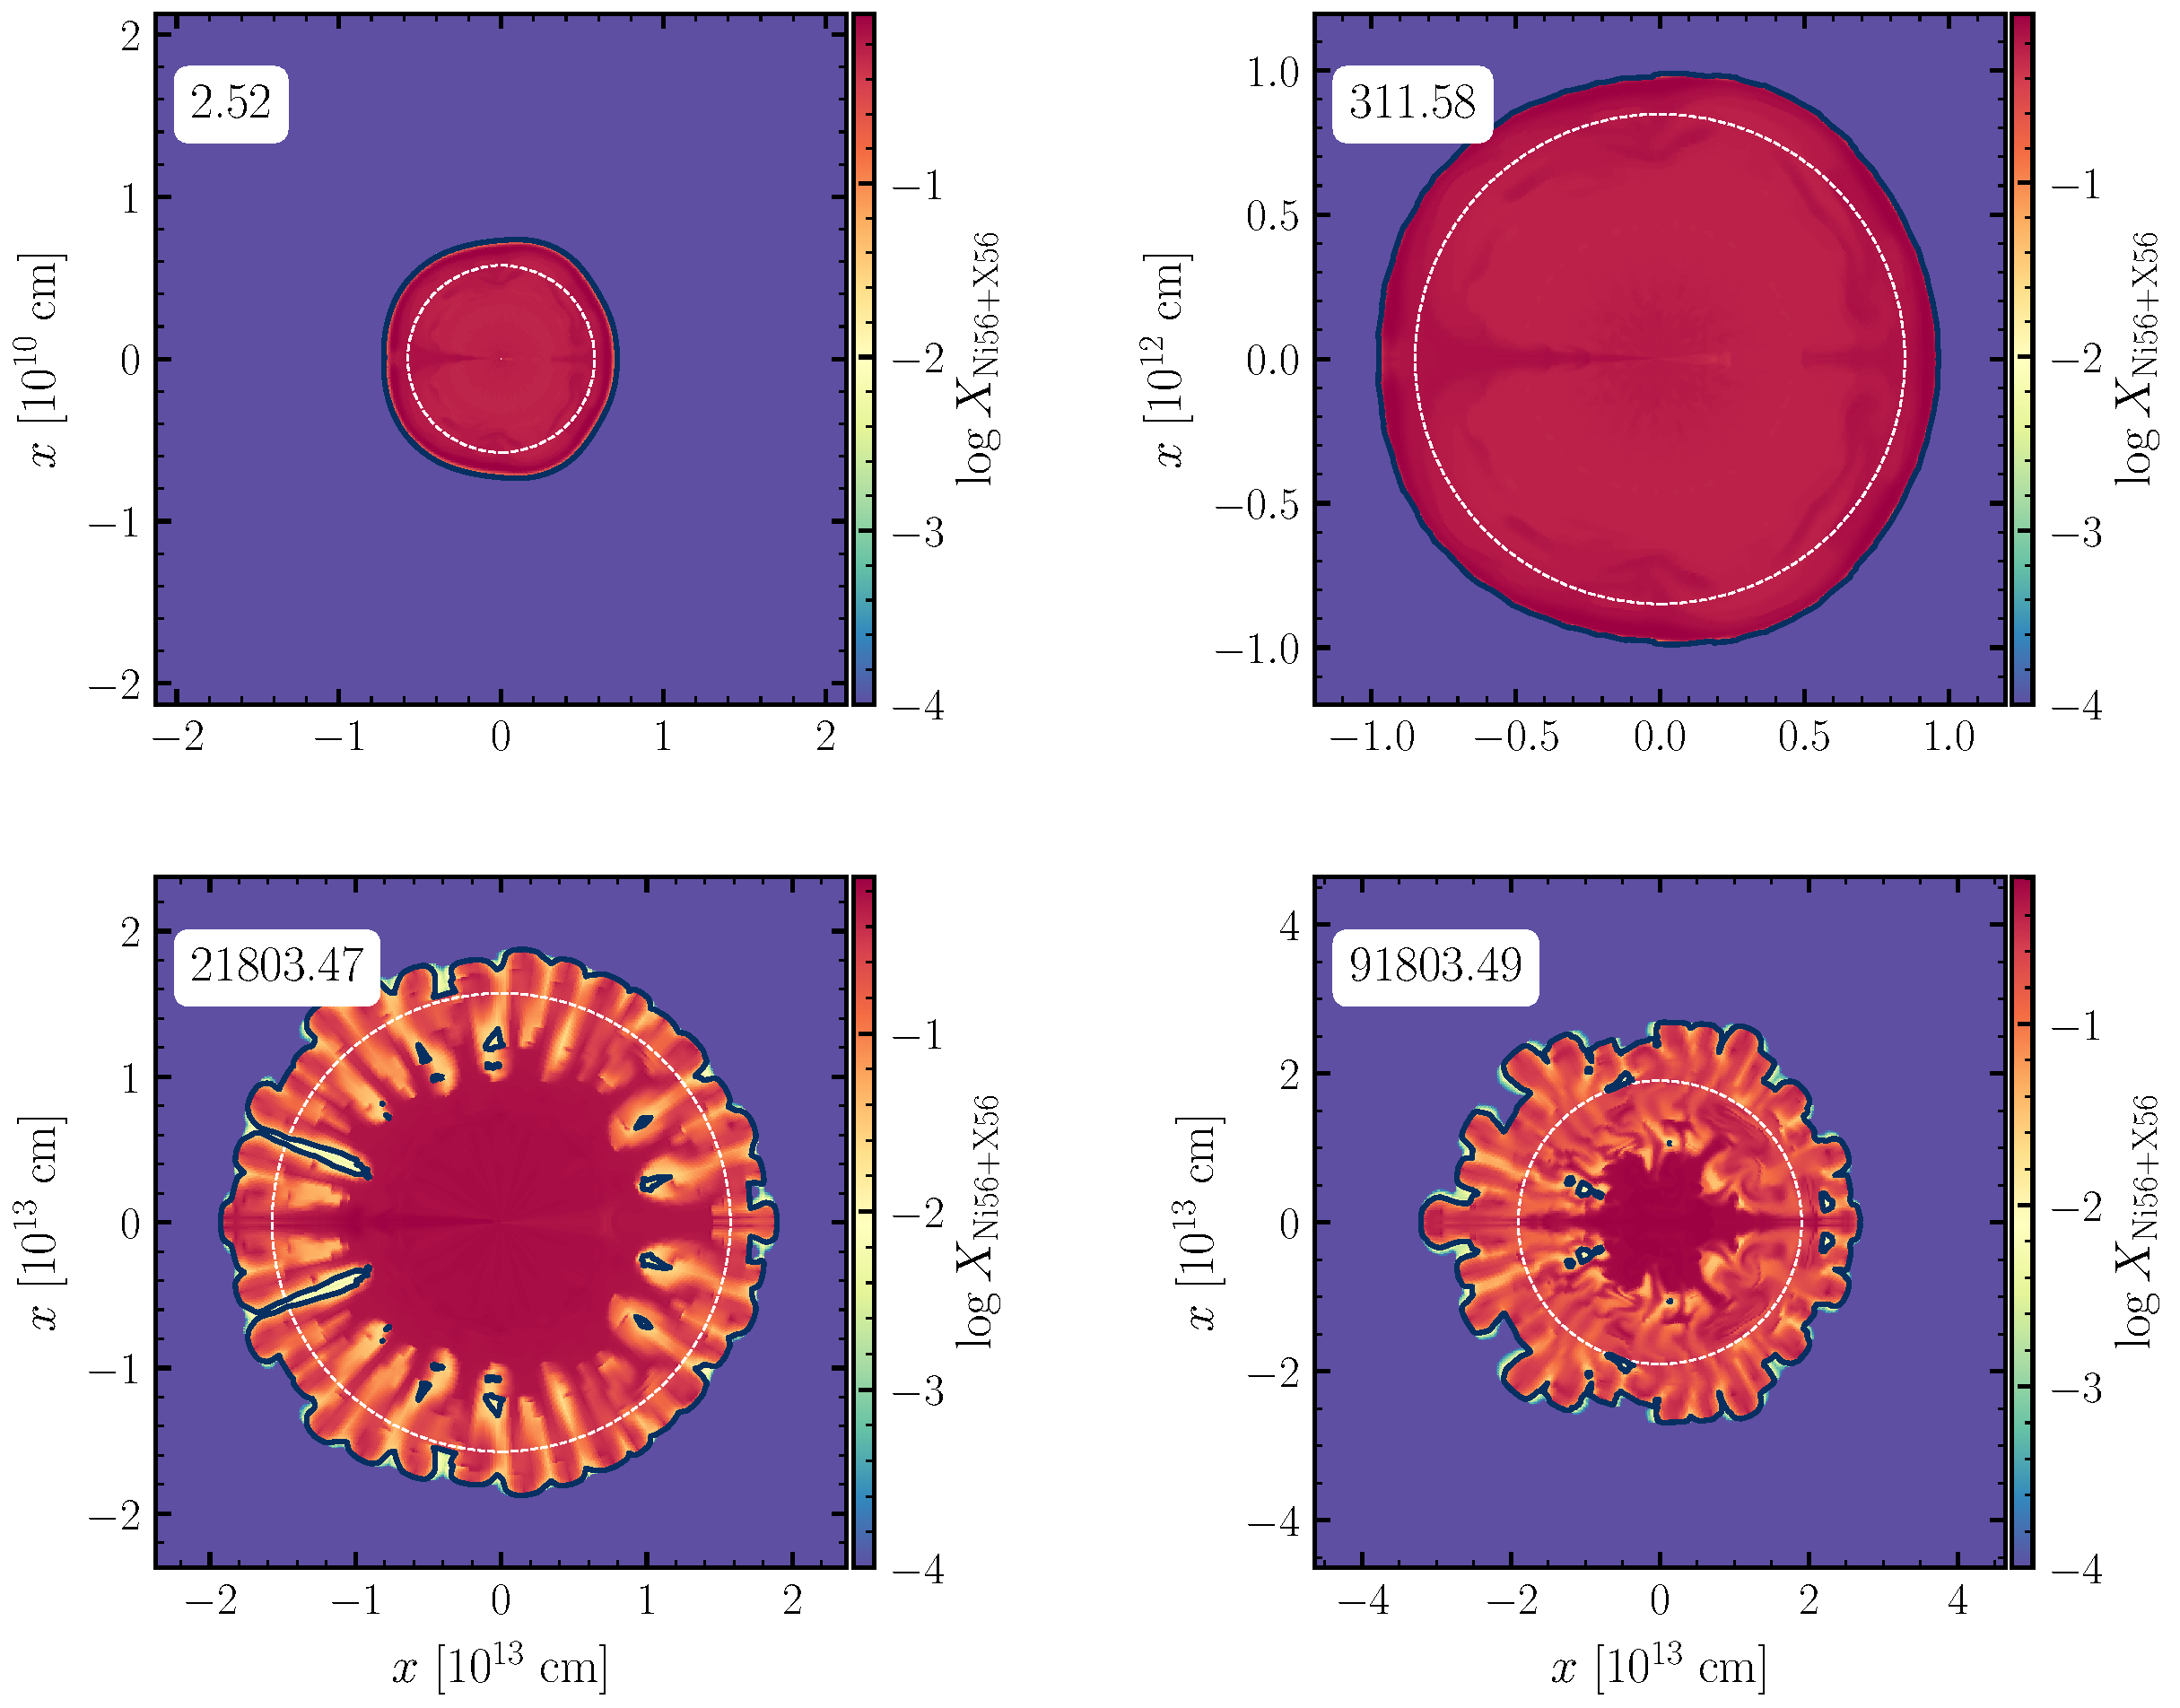
\includegraphics[width=0.8\textwidth]{pic/species_cuts_e10_2d_4times.pdf} 
 \caption{Planar cuts through the $e8.8_{\mathrm{2D}}$ model at the indicated times showing the \nickel+\tracer mass fraction. The black contour line gives the \nickel+\tracer = 0.1 surface, whereas the dashed white line denotes the mass coordinate of the former He/H interface. Expansion happens self similarly over until first RT fingers grow at the interface. These fingers grow to their maximal radial extent when the reverse shock, located at the lower end of the RT fingers in the lower left panel, travels back to the center of the star. \textcolor{red}{REPLACE WITH 3D result!}}
 \label{fig:e8_3d_species_4times}
\end{figure*}

% reverse shock
As the reverse shock begins to fall back into the center, the RT-fingers grow to their maximal radial extent. This can be seen in the lower left and lower right panels in \autoref{fig:e8_3d_species_4times} where we show the logarithm of the \nickel + \tracer mass fraction. The reverse shock is situated at the lower end of the RT-Fingers in the lower left panel showing a snapshot at $t_{\mathrm{pb}}=21803\;\mathrm{s}$. Indicated by the white dashed circle is the mass coordinate of the former He/H interface.
During this phase the formerly thin spherical \nickel-shell is completely smeared out by these fingers and mixed into the underlying neutron rich material in radius and velocity distribution. 

Since most of the iron group nuclei remain within the high density shell until the reverse shock runs over the inner layers, their deceleration is enormous. This is shown in the lower two rows in \autoref{fig:e8_massDis_4times}. Where most of the iron rich material has velocities of $v_{\mathrm{Ni,X}}\approx 30\times10^3 \;\mathrm{km/s}$ at $t_{\mathrm{pb}}=300\;\mathrm{s}$ these layers are decelerated to $v_{\mathrm{Ni,X}}\approx 2.5\times 10^3\;\mathrm{km/s}$ within some $5 \;\mathrm{h}$. The lower velocity tail of the iron group elements even lays in negative velocity space. 
Compression of the innermost ejecta by the reverse shock is also evident in the distribution over mass coordinate. Where a small fraction of the neutrino heated ejecta is mixed to $M(r)=1.4\;\mathrm{M_{\odot}}$ until $t_{\mathrm{pb}}=\;21.800\;\mathrm{s}$, the bulk resides still at  $M(r)=1.35\;\mathrm{M_{\odot}}$ clearly separated from the carbon and oxygen that extends to $M(r)=1.47\;\mathrm{M_{\odot}}$ and is evenly distributed over the whole post shock region.

% reflection of the reverse shock
The last phase is characterized by the reflected reverse shock that overruns the inner metal rich ejecta from the inside out. Due to the deformation of the reverse shock by the RT-fingers, the focal point of the reflection is not exactly at the center of the computational grid. This causes matter behind the reflected shock to be deflected at its surface  increasing the lateral velocities in the central material and disrupting the RT-fingers. When the reverse shock has passed the inner ejecta they are left almost fully mixed in radius and velocity as can be see in the last row of \autoref{fig:e8_massDis_4times} and in the lower right panel of \autoref{fig:e8_3d_species_4times}.

% Figure e8.8 mass distribution
\begin{figure*}
 \centering
 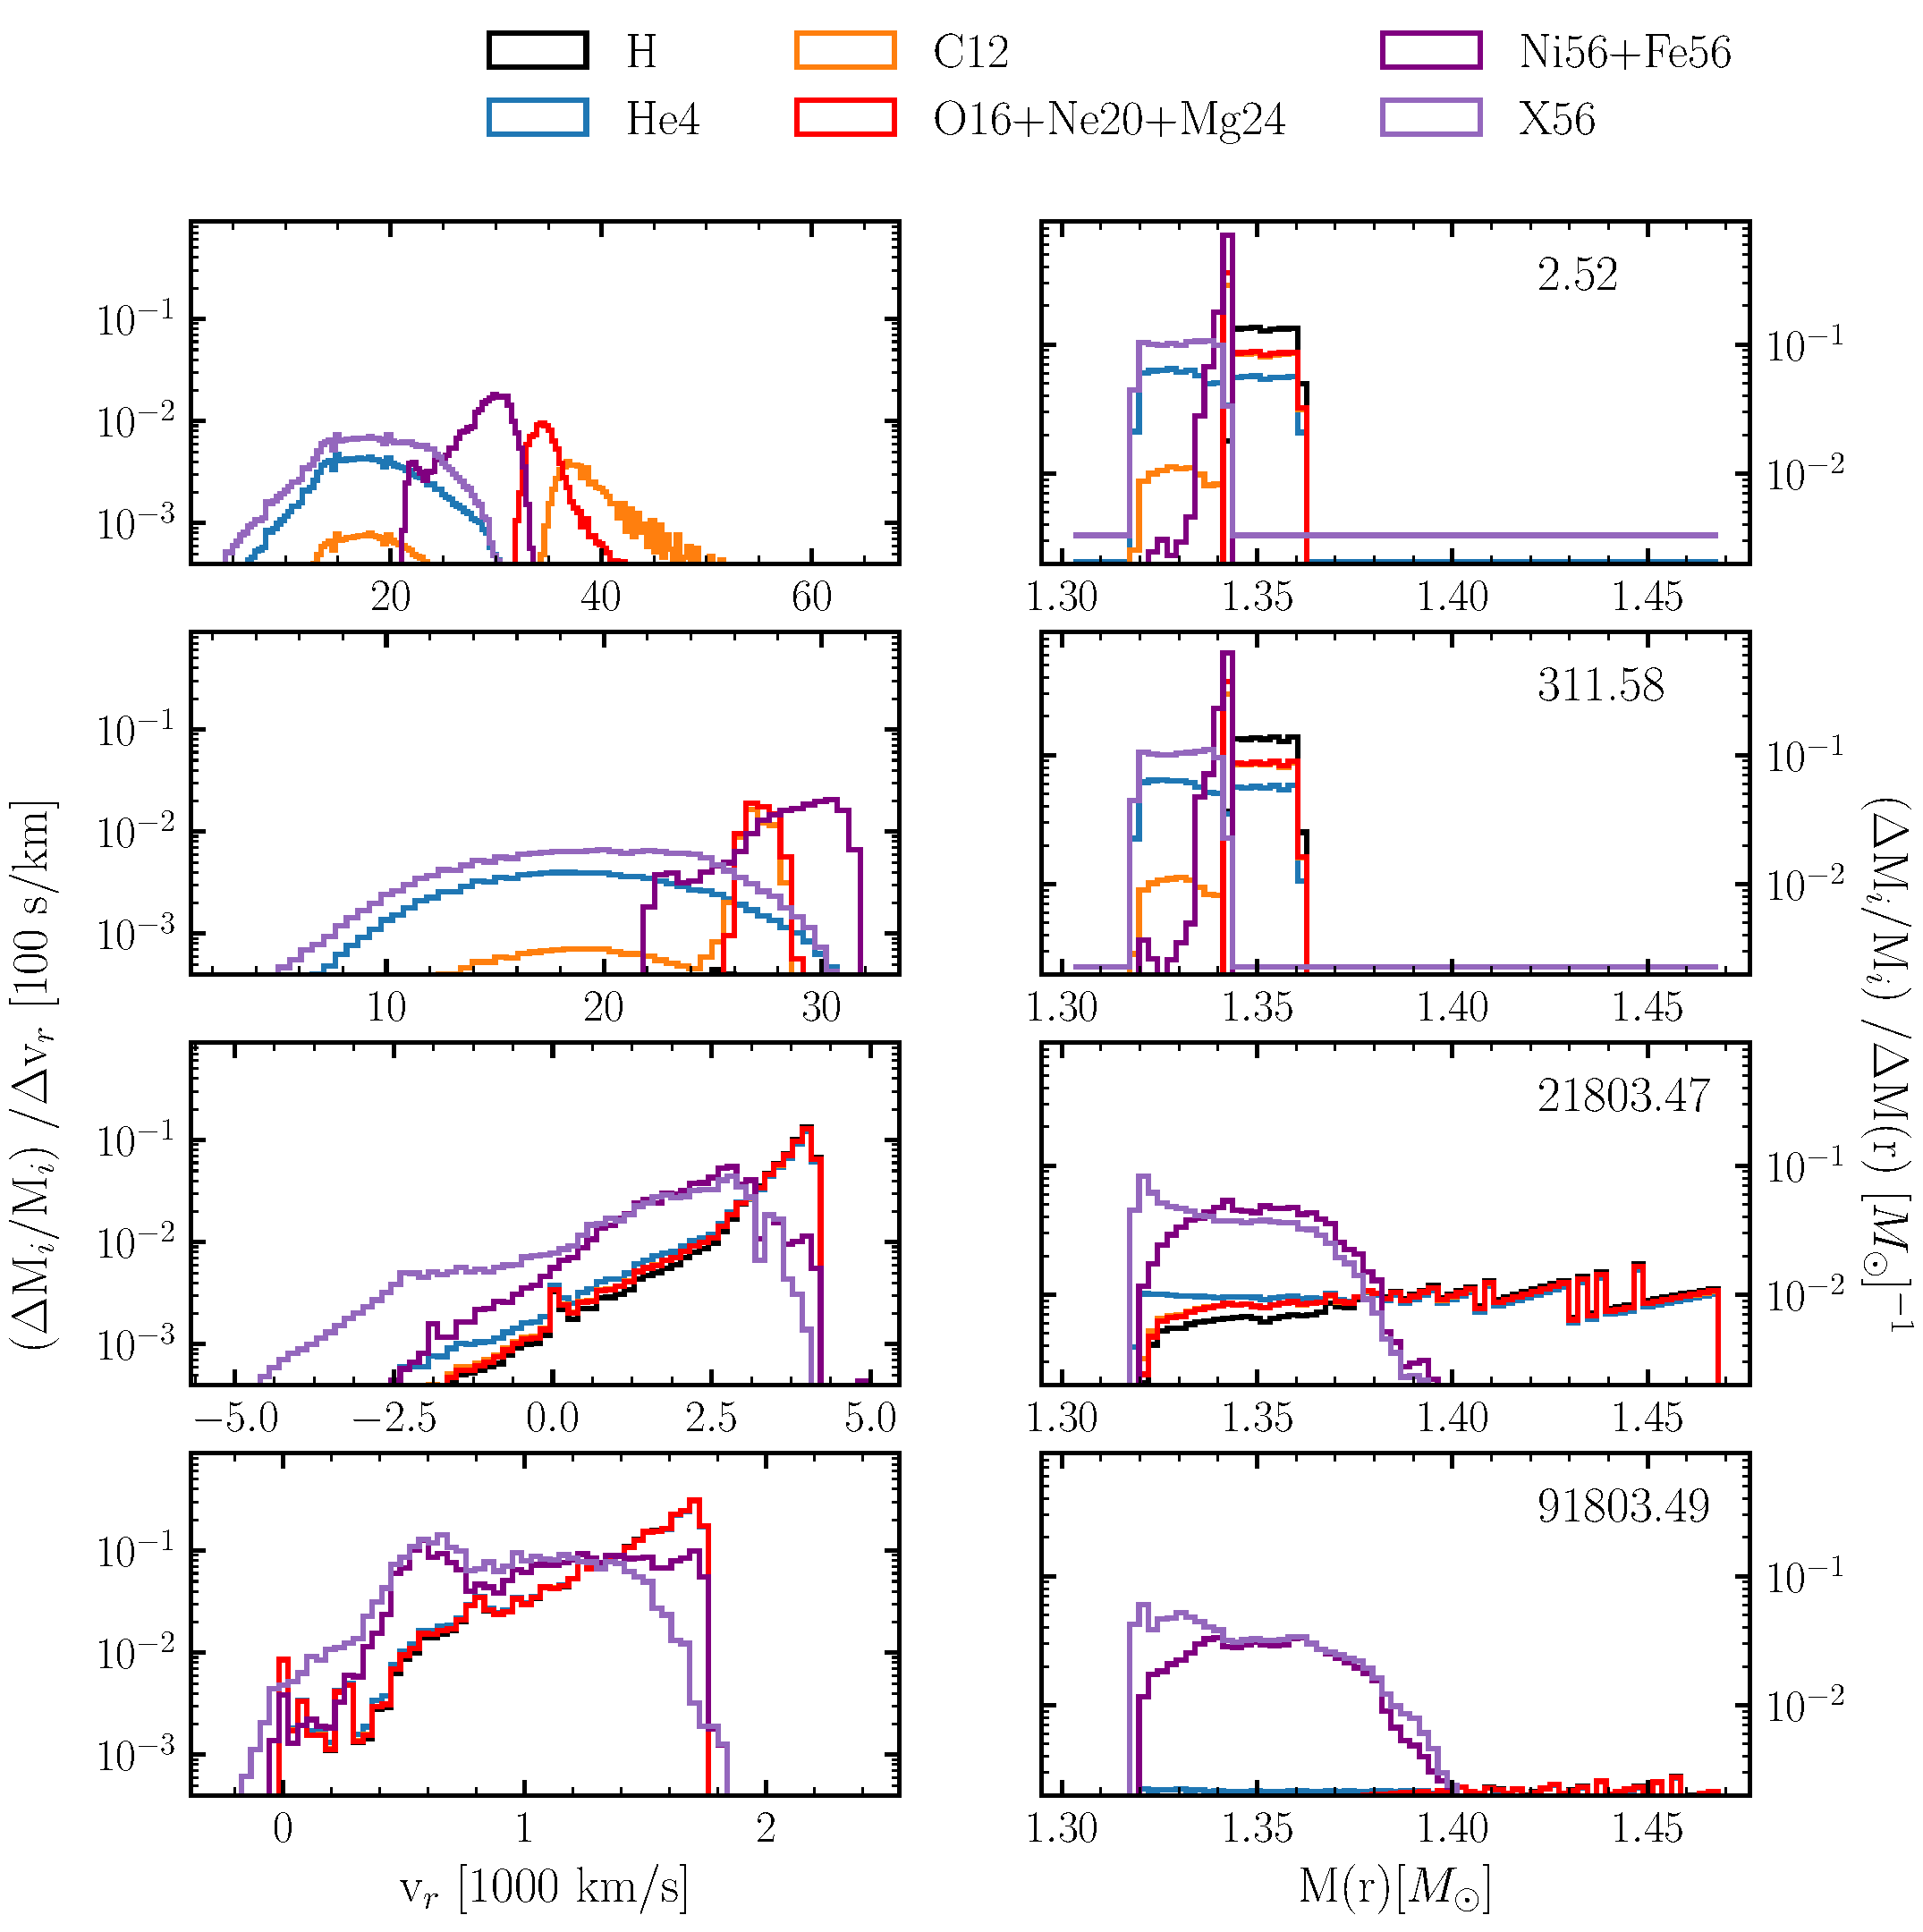
\includegraphics[width=0.9\textwidth]{pic/e8_10_mvr_mas_4times.pdf}
 \caption{Mass distributions of elements in velocity and mass space  of the $e8.8^{\mathrm{2D}}_{10}$ model at the indicated post bounce times. We cover the initial state as we start our long term simulation in the uppermost panel, over the time the reverse shock passes the ejecta (second and third panels) and the distribution at late times.}
 \label{fig:e8_massDis_4times}
\end{figure*}

%post shock breakout
After shock breakout the very first stage of the remnant evolution begins. As long as the ejecta mass is larger as the circumstellar - mass (CSM) swept up by the forward shock one speaks of the ejecta dominated (ED) phase. Various analytical studies regarding shock evolution and growth of instabilities have been focusing around this phase (see e.g. \cite{Truelove1999EvolutionRemnants} for a general approach or focused around the crab \cite{Chevalier1984TheSurroundings}).  It is also the phase where, after radioactive decay has powered the plateau phase of type II supernovae, the medium becomes optically thin and the remnant moves into the nebular phase. Here velocity distributions also of the heavy elements can be inferred by spectral analysis of the ejecta.

\subsection{Multidimensional long term simulations of the $z9.6$-Model}
\label{subsec:muldidimensional longterm z9}
The first seconds after we start our long term simulation of the $z9.6$ the dynamics is dominated by the neutrino driven wind, similar to the one dimensional simulation. It blows into the low density bubble produced by the explosion, accelerating the core material that eventually is decelerated in the immediate post shock region forming the wind termination shock. 
% Shock Propagation and Instabilities
Since during this time the forward shock propagates through the CO core where the $\rho r^3$ profile is smooth the ejecta expand self similarly. 

% Figure Z9.6 species cuts
\begin{figure*}
 \centering
 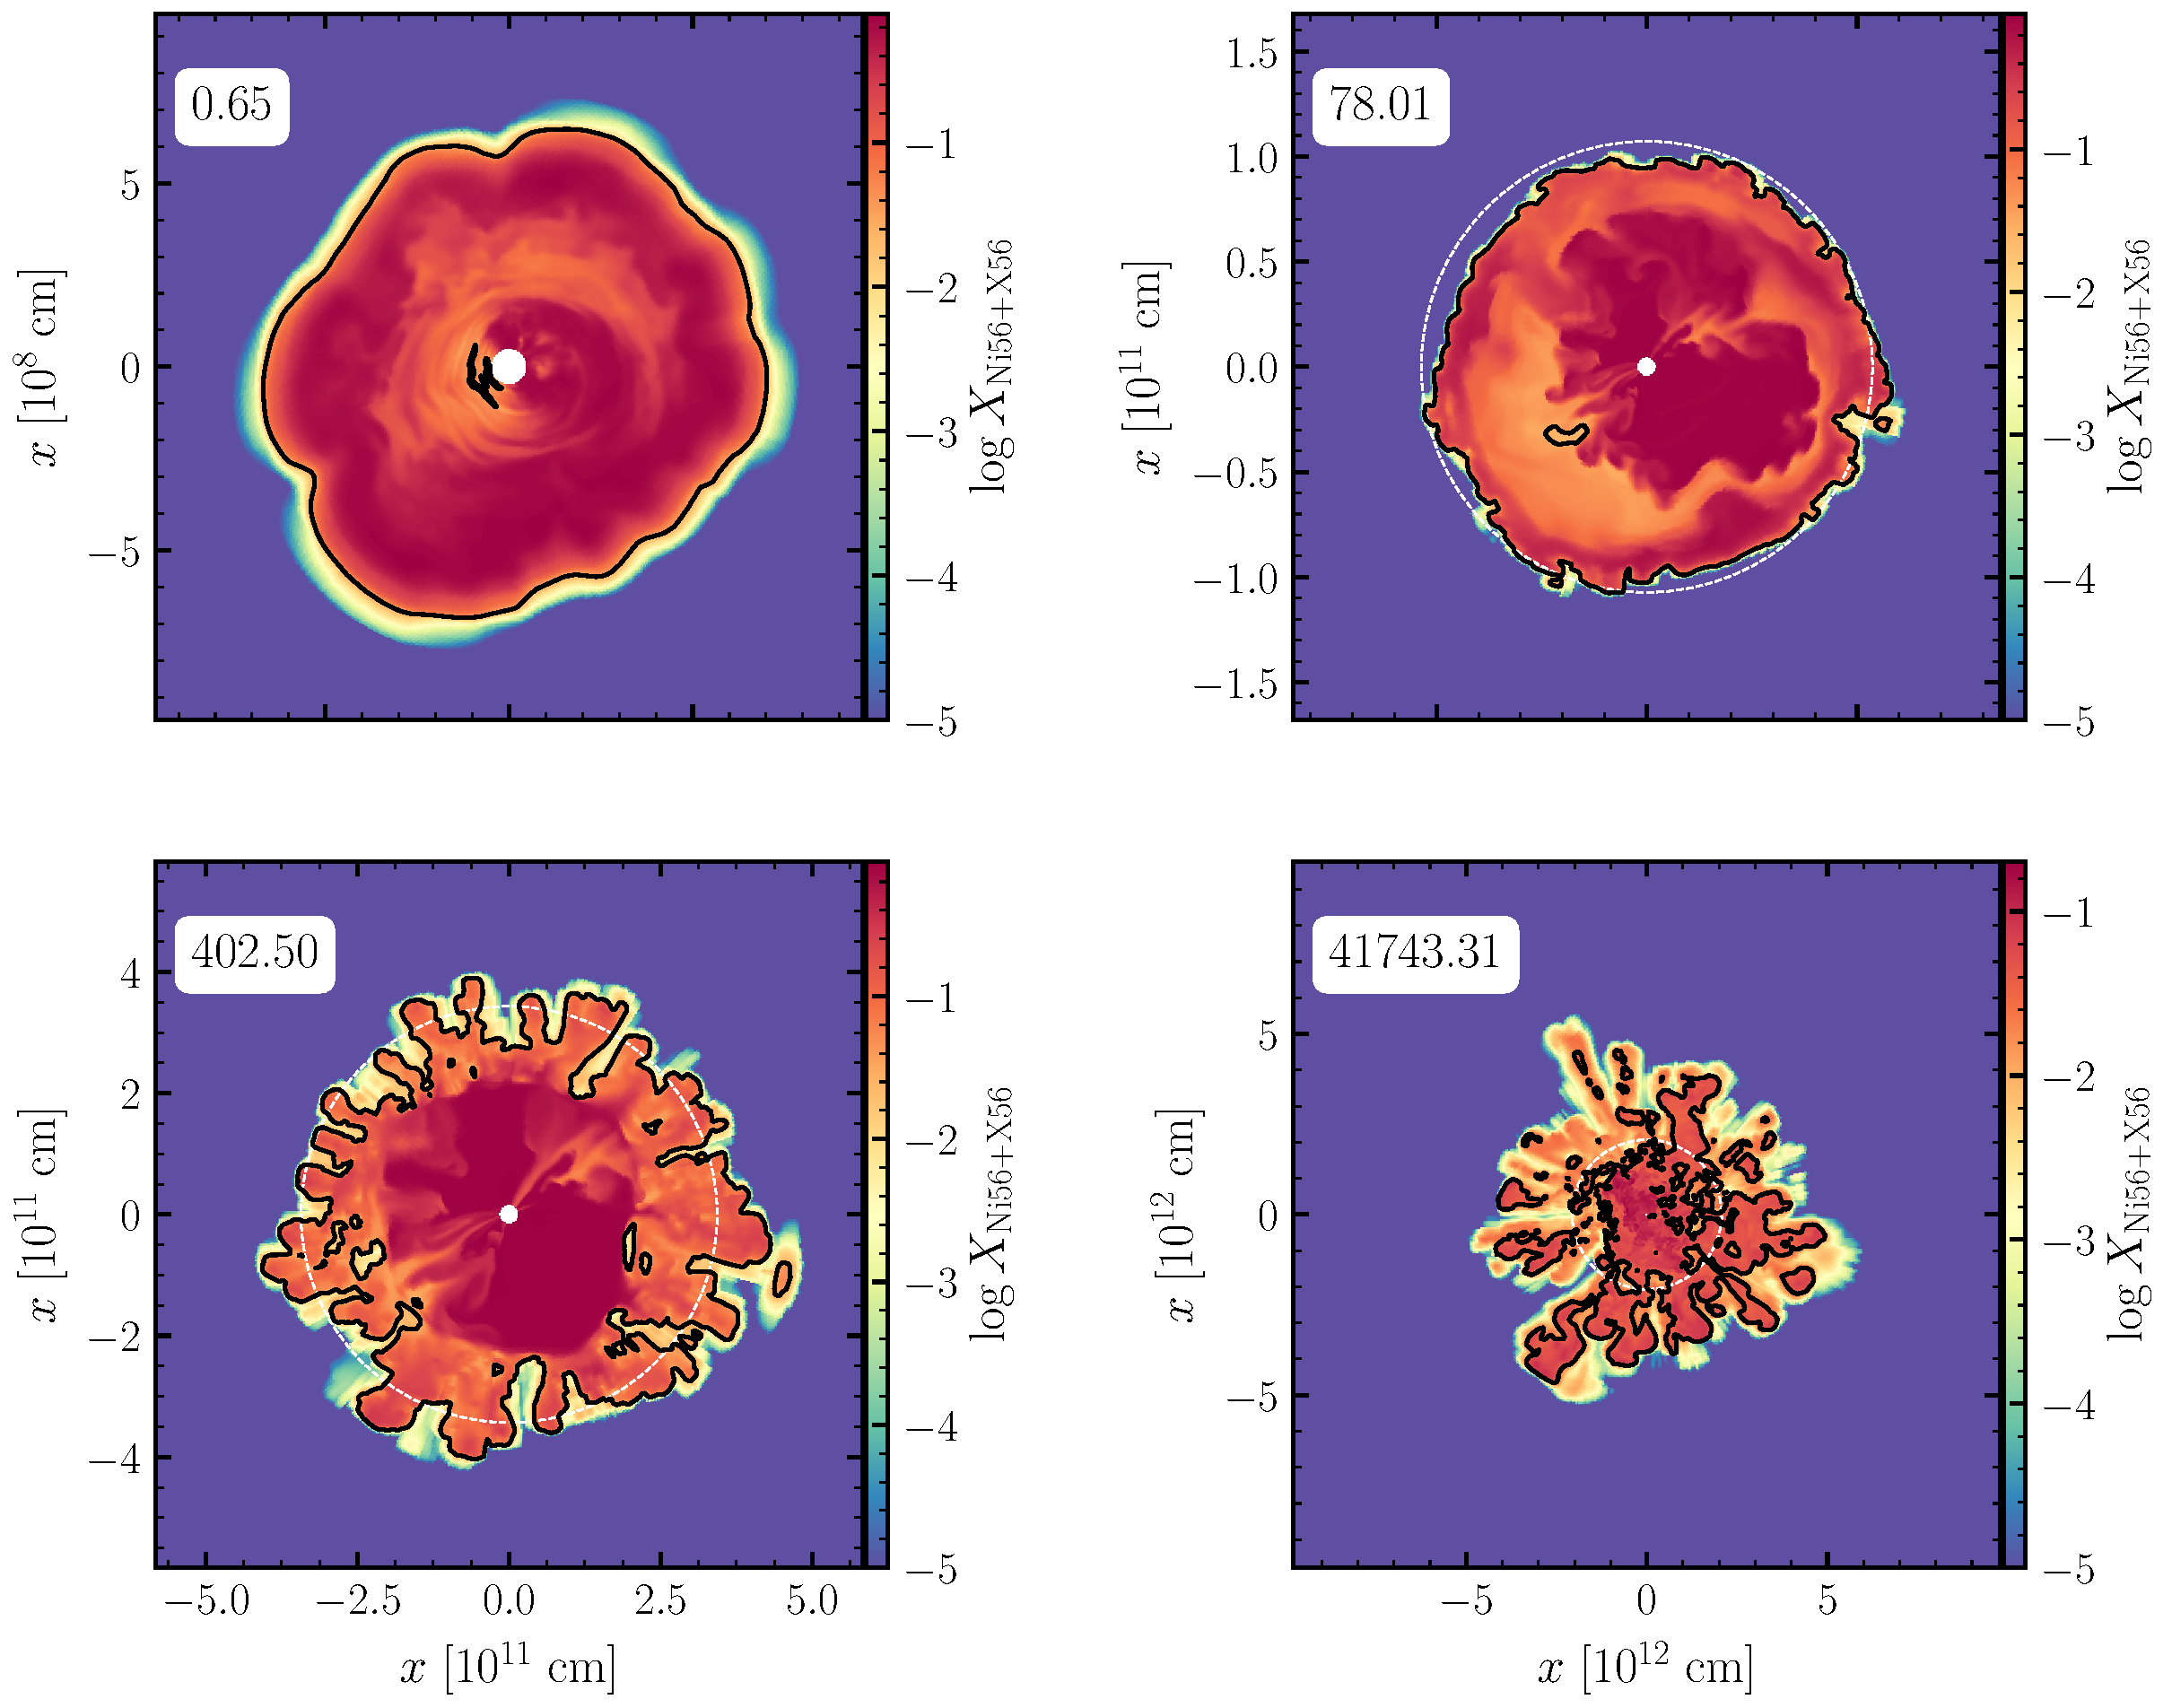
\includegraphics[width=0.9\textwidth]{pic/species_cuts_z9_3d_4times.pdf}
 \caption{Planar cuts through the $z9.6_{\mathrm{3D}}$ model at the indicated times showing the \nickel+\tracer mass fraction. The slices are adjusted such that the \textit{initial} maximum mass flux of the shown species is directed southward. The contour line gives the iso-surface of \nickel+\tracer=2\%. Initially the \nickel+\tracer distribution is fairly spherical with small deformations in the south-western direction. These deformations are reduced as the material expands. First RT-cusps are visible at $t_{\mathrm{pb}}\approx 78\;\mathrm{s}$. In the lower left panel, showing the state of affairs at  $t_{\mathrm{pb}}\approx 400\;\mathrm{s}$ the reverse shock, visible as the reddish discontinuity at $r\approx 2\times 10^{11}\;\mathrm{cm}$ already travels back in radius. }
 \label{fig:z9_3d_species_4times}
\end{figure*}

The outermost metal rich ejecta arrive at the former CO/He interface (located at $\sim1.372$\solm) at $t_{\mathrm{pb}}\approx 73\;\mathrm{s}$.  As can be seen in the right upper panel of \autoref{fig:z9_3d_species_4times} the self similar expansion is terminated by the growth of the first Rayleigh-Taylor plumes. This is in line with the linear stability analysis presented in \autoref{subsubsec:Linear Stability Analysis}. Note that these initial fingers grow in a region confined between the forward shock and a dense shell that has formed due to the deceleration of the shock in the CO and He core. Most of the metal rich ejecta are located behind this dense wall. Additionally, and in line with theory, the plumes have a fairly small angular size as they grow from small scale perturbations at the interface. 

While the fingers grow during the next $300-400\;\mathrm{s}$ the continuous deceleration of the shock in the He core sends pressure waves back into the post shock material that steepens into a reverse shock. The position of the reverse shock is clearly visible in the deep red region in the lower left panel of \autoref{fig:z9_3d_species_4times}. Since only very little mass of iron and other heavy nuclei can be mixed into the He core before the reverse shock forms the large deceleration caused by the back propagation of the reverse shock affects the metal rich ejecta the most.
At around $t_{\mathrm{pb}}=1500\;\mathrm{s}$ the reverse shock reaches our inner boundary and is reflected back into the core material.
Similar to the one dimensional simulation nonlinear waves perturb the innermost ejecta distorting the Rayleigh-Taylor fingers that reached down to the inner boundary. Since the reflected wave cannot catch up with the fastest shrapnels that originated from the growth of RT plumes at the CO/He interface it dos not influence the high velocity iron rich ejecta.
After these dynamics events the forward shock reaches the He/H interface at around $t_{\mathrm{pb}}=2000\;\mathrm{s}$. Since the core envelope transition is very smooth and the post shock density rather uniform, no additional growth of the RTi is to be expected. Accordingly the plumes that grew from the CO/He interface propagate unimpared with the background flow. 
% Figure Z9.6 mass distribution
\begin{figure*}
 \label{fig:z9_massDis}
 \centering
 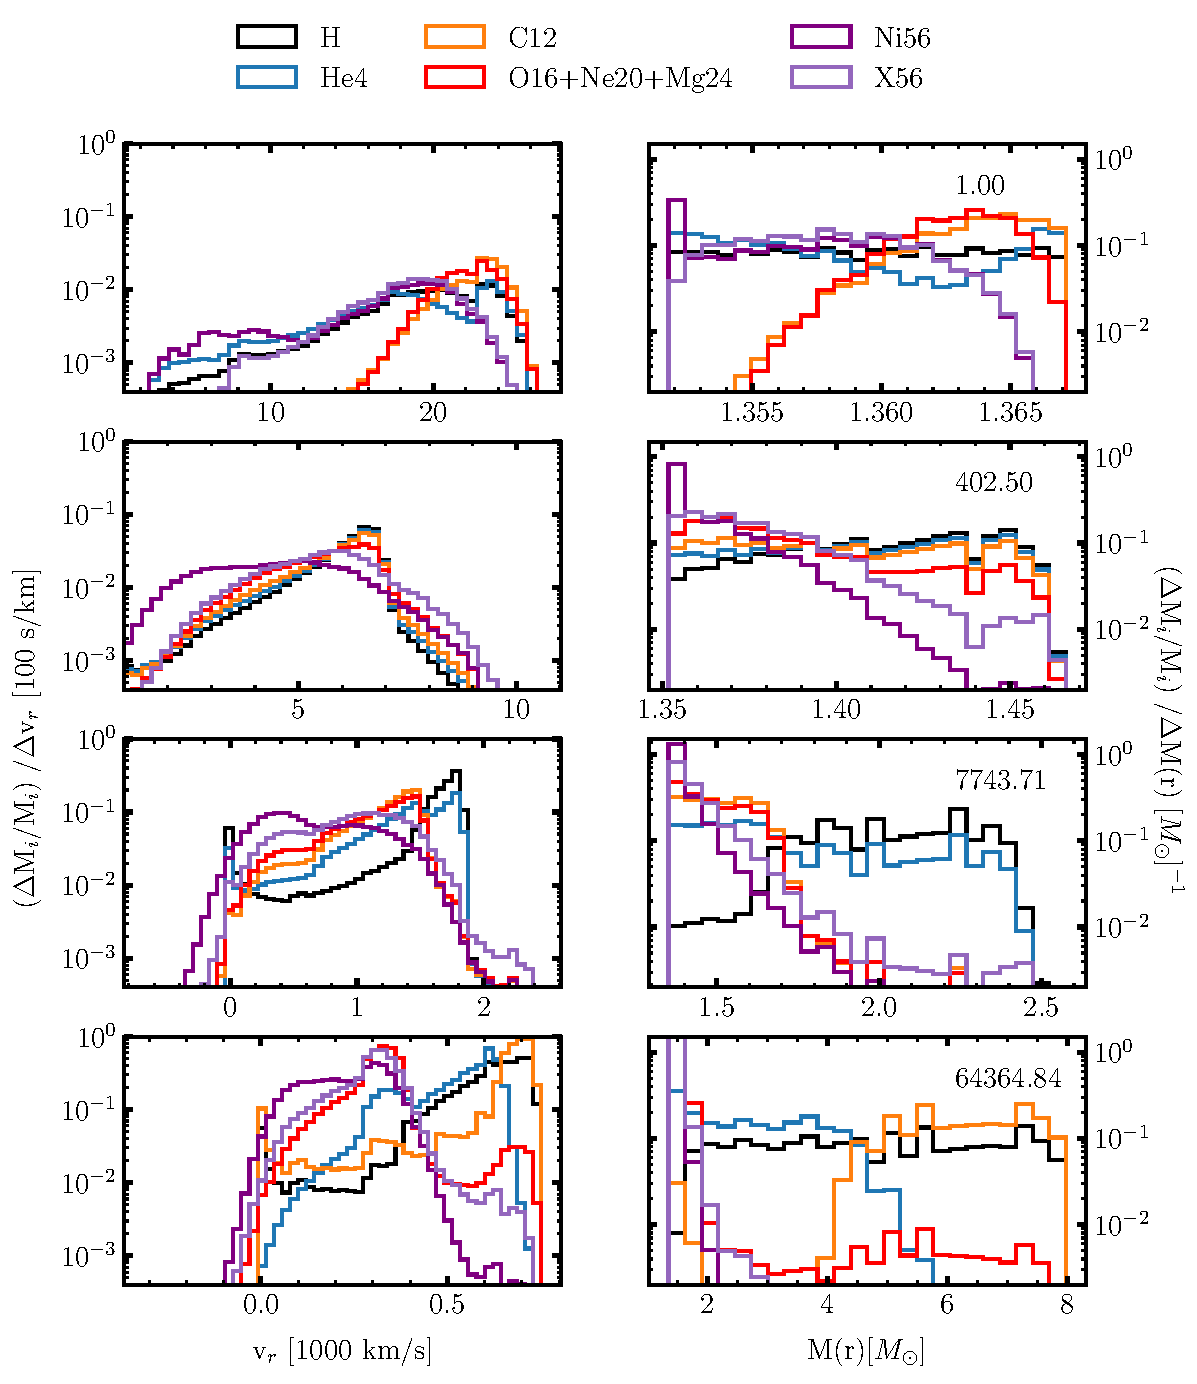
\includegraphics[width=0.9\textwidth]{pic/z93_3d_old_massDis_mvr_mas_4times.pdf}
 \caption{Same as \autoref{fig:e8_massDis_4times} but for the $z9.6_{\mathrm{3D}}$. We cover the initial state as we start our long term simulation in the uppermost panel, over the time the reverse shock passes the ejecta (second and third panels) and the distribution in the hydrogen envelope as the ejecta expand self similarly.}
\end{figure*}
% Mass Velocity Distribution
As has been stated before the early formation of the dense shell has important consequences for the velocities the  metal rich ejecta can achieve and how far they can be mixed into the envelope.
In \autoref{fig:z9_massDis} we show the distribution of elements over mass and velocity space for the $z9.6$ model at the same snapshots as shown in \autoref{fig:z9_3d_species_4times} to illustrate the influence of the reverse shock and the dense shell onto the ejecta.

Compression of the ejecta in velocity space and some mixing over mass coordinate can be observed from the upper to the second row of \autoref{fig:z9_massDis} showing snapshots at $t_{\mathrm{pb}}=0.65\;\mathrm{s}$ and $t_{\mathrm{pb}}=78\;\mathrm{s}$. The compression is caused by the strong deceleration of the forward shock in the stellar material, reducing the initial maximal velocities from $v\approx 25\times10^3\;\mathrm{km/s}$ down to $v\approx 12.3\times10^3\;\mathrm{km/s}$, whereas the first plumes that rise from the CO/He interface mix a tiny amount of iron rich ejecta into the He core. Note however that the reverse shock travels with $v_{\mathrm{rev}}\approx 10.6\times10^3\;\mathrm{km/s}$ at $t_{\mathrm{pb}}=78$ and the bulk of \nickel and \tracer travels with smaller velocities of $v\approx 9\times10^3\;\mathrm{km/s}$. This behaviour of the model is again similar but less extreme as found in the ECSN model.

As the RT plumes grow over the course of the following $300\;\mathrm{s}$ they continuously mix \nickel and \tracer into the He core. This is visible in the third row left column of \autoref{fig:z9_3d_species_4times}. At the same time the reverse shock forces the bulk of the metal rich ejecta to even lower velocities of  $v\approx 6\times10^3\;\mathrm{km/s}$. 

\subsection{Multi-dimensional long-term simulations of the $s9.0$-model}
\label{subsec:Multi-dimensional long-term simulations of the s9.0-model}
\COM{Growth of RTi at He/H}
\COM{Initial perturbations growing from passage of O interfaces}

\subsubsection{Dependence on the explosion energy}
\label{subsec:Dependence on the explosion energy}
% e8.8
Although the explosion energies for the e8.8 model cover over one magnitude differences in mixing of species in radius and velocity are minor. At $t_{\mathrm{pb}}\sim 2.5 \;\mathrm{s}$ the velocity distribution of elements is almost identical. Small differences are visible in the maximum velocities achieved and are higher for higher explosion energy. Mixing in mass coordinate follows a similar pattern with slightly more \nickel mixed into the neutron rich material for more energetic explosions. This is a relic of the pronounced down flows seen in the models $e8.8_{10}$ and $e8.8_{15}$. 
Inspecting later times ($t_{\mathrm{pb}}\sim 8 \;\mathrm{h}$) the findings still show similar behaviour. \nickel is mixed over a slightly larger fraction of the total ejected mass for the higher explosion energies. Differences in the velocity distribution are only visible in the lower tail with negative velocities. 
At 200 days after the explosion the velocity distributions are besides the maximum reached velocity basically identical.
\begin{figure}
 \label{fig:e8_massDis_32d}
 \centering
 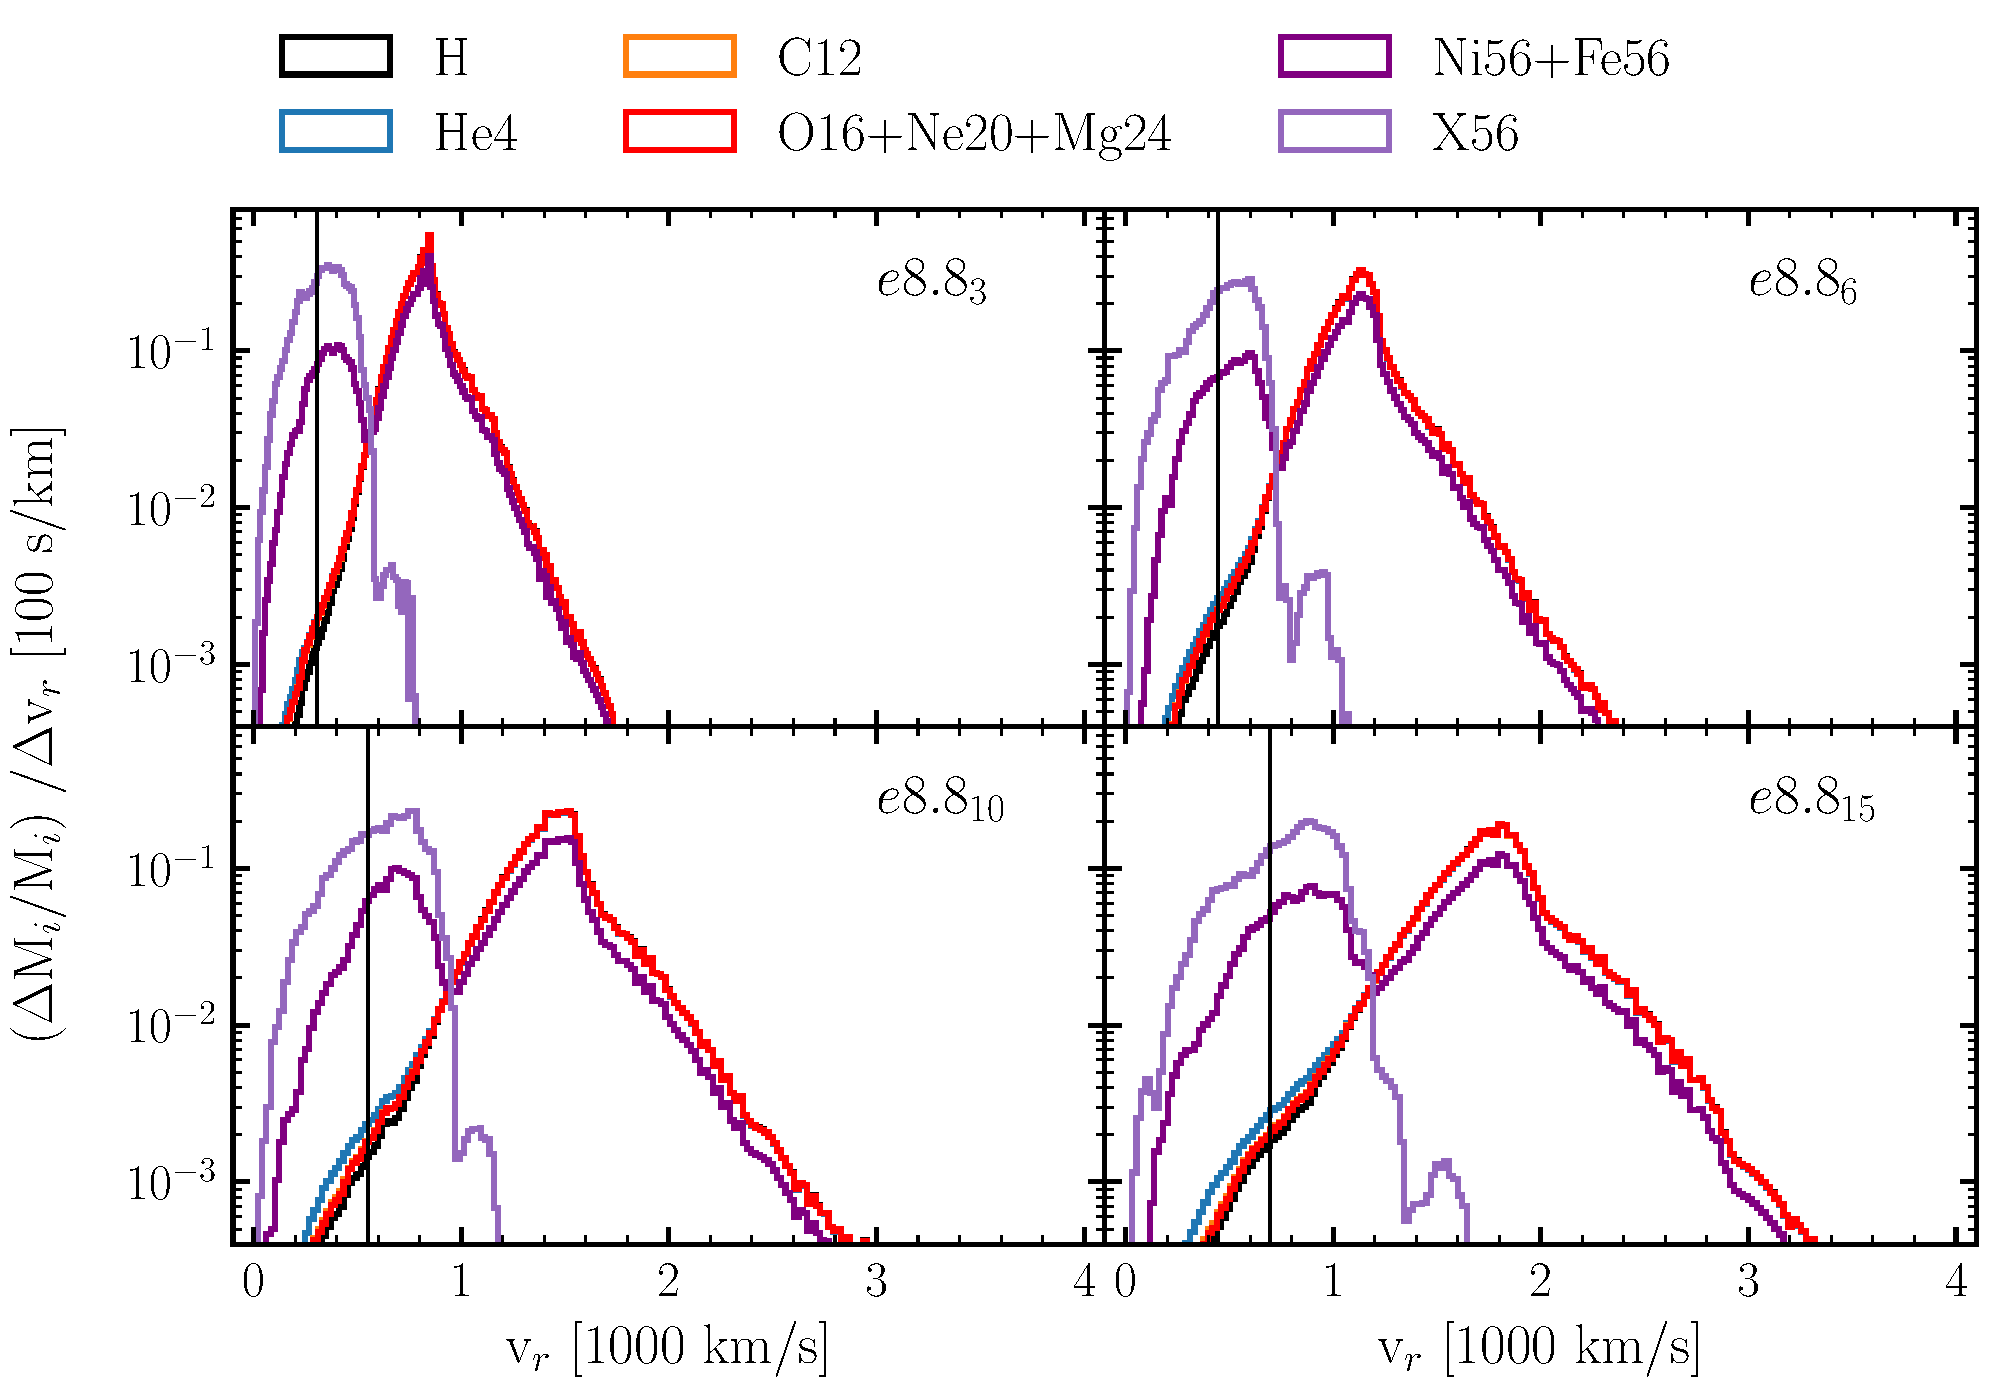
\includegraphics[width=0.49\textwidth]{pic/massDis_mvr_all_time_200d.pdf}
 \caption{Mass distributions of elements in velocity space at 200 days p.b. for the two dimensional models. We used 200 bins evenly distributed from  $0-4\times 10^3\;\mathrm{km/s}$. Due to the almost spherical explosion heavy elements are just slightly mixed into lighter material, as visible for \tracer in the region between $0.5-1\times 10^3\;\mathrm{km/s}$. The vertical black line denotes the position in velocity space where $(\Delta M_{\mathrm{i}}/M_{\mathrm{i}})/\Delta v_{\mathrm{r}}$ first exceeds $1\times 10^{-3}\;\mathrm{100\;s/km}$ in our 1D simulations.}
\end{figure}
% iron cores
As the ion core progenitors are exploded self consistently their explosion energy is fixed within our framework. Drawing direct connections between the amount of mixing and the explosion energy can therefore not be done. Comparing the $z9.6$ model with electron-capture model, that have similar explosion energies, hints that the influence is minor however. Decisive for the amount of nickel mixing is the progenitor structure and initial perturbations after shock revival. This view is supported by the strong mixing apparent in the $s9.0$ model that has comparable explosion energy as well. The initial density perturbations combined with the strong de- and acceleration of the forward shock in the envelope of the progenitor yields high growth-rates over a larger space in mass coordinate. 

\subsubsection{The effect of $\beta$-Decay}
After a few days, when the shock sweeps through the circumstellar material (CSM), the decay of radioactive \nickel can become dynamically important. The so called Ni-Bubble effect emerges when the energy input by \nickel decays pushes the surrounding material aside into dense shells and leaving low density cavities in the ejecta. The strength of the Ni-Bubble effect, and thus the increased velocity of the ejecta $\mathrm{v}_1$,  can be estimated (\cite{Chevalier2005} ) assuming that \nickel resides in a central region of constant density by
\begin{equation}
\mathrm{v_1} = 975\Big(\frac{\mathrm{M_{Ni56}}}{0.1\mathrm{M_{\odot}}} \Big)^{1/5} \Big( \frac{\rho_a t^3} {10^9 \mathrm{\;g\;s^3/cm^3}}\Big)^{-1/5} \mathrm{[km/s]}
\end{equation}
where $\rho_a$ is the density of the ambient medium. Given that the electron capture model only produces \nickel masses of the order of $10^{-3}\;\mathrm{M_{\odot}}$, the total energy available due to $\beta$-decays is only $\sim 10^{47}\;\mathrm{erg}$, thus acceleration by the Ni-Bubble effect will be minor and of order a few $10\;\mathrm{km/s}$.

\begin{figure}
 \label{fig:e8_beta}
 \centering
 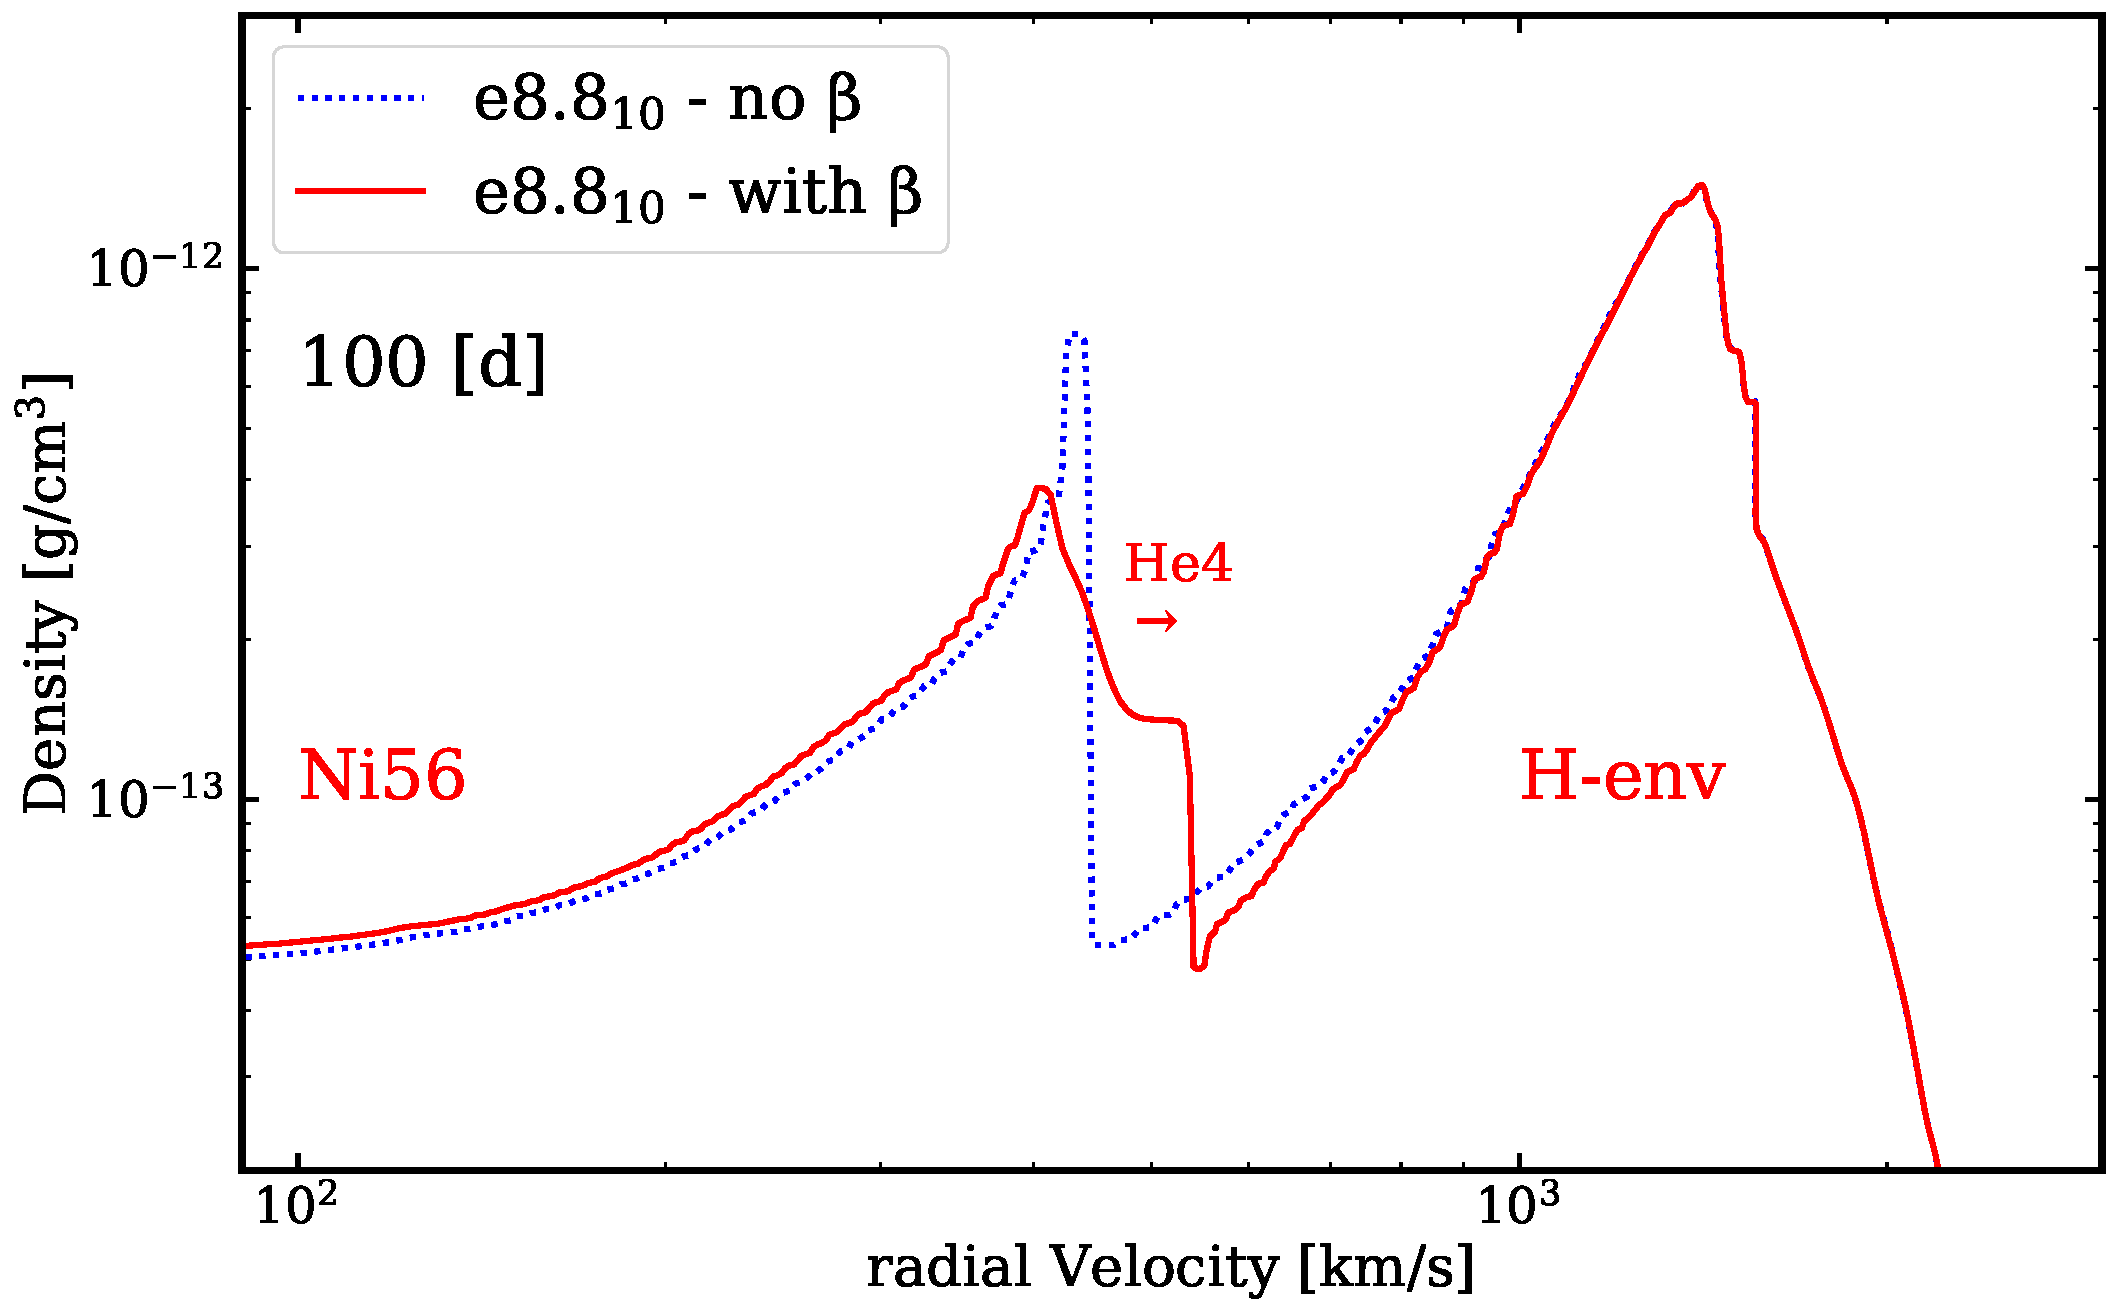
\includegraphics[width=0.49\textwidth]{./pic/e8_10_beta_nobeta_den_vs_vr.pdf}
 \caption{Density profile of the $e8.8_{10}$ ejecta 100 days p.b.. The model including $\beta$-Decay is depicted in red, the model without in blue. Marked is the \helium rich region that is pushed outward by the decaying \nickel. }
\end{figure}

\section{Comparison to previous studies}
\label{sec:Comparison to previous studies}

Previous studies like the ones of \cite{Hammer2010}, \cite{Joggerst2010}, \citet{Wongwathanarat2015}, \citet{Kifonidis2005} also performed long time evolution of CCSNe to explore to extend of mixing and the influence of the RTi on the velocities of the ejecta. \cite{Hammer2010} used a 15 \solm blue supergiant, while \cite{Joggerst2010} used three different 15 \solm progenitors with different metallicities. Also \cite{Wongwathanarat2015} deployed various models from 15 - 20 \solm using \prom. These studies aimed to explain the fast nickel observed in SN 1978A.
A main caveat in the study by \cite{Joggerst2010} is the artificially induced explosion with a piston to give an explosion energy of $2\times 10^{51}\;\mathrm{erg}$, thus neglecting the initial instabilities arising from convective overturn during the first seconds of the explosion. Mixing in their model is exclusively caused by the RTi developing at the composition interfaces whereas the model by \cite{Hammer2010} inherited seed perturbations arising during the initial shock acceleration. This is also the case for the simulations by \cite{Wongwathanarat2015} making a comparison to these studies more suggestive.
Interestingly the models by \cite{Wongwathanarat2015} show similar mass-velocity distributions over every species at breakout time. The bulk of the material from He to Ni in their B15 model e.g. moves with velocities of up to 3000 \kms without large differences per species. There is also no bimodal feature seen in the O-rich ejecta. Considering our $z9.6$ model ONeMg rich material shows a clear bimodal feature short before shock breakout. Also C-rich matter is expelled faster than the models by \cite{Wongwathanarat2015} would suspect. Additionally we do not find a fast moving tail in all species as it is found in all of their models. 

\section{Conclusions and Outlook}
In the present paper we explored the long term evolution of the explosion  low mass 

%-----------
% APPENDIX
% --------------
\begin{appendices}
\section{Progenitor details}

\begin{table}
   \begin{tabular}{l l l l} 
   \hline
     Model      &Interface & $\mathrm{R_{Prog}\;[cm]}$ & $\mathrm{M_{prog}\;[M_{\odot}]}$ \\ [0.5ex] 
   \hline
   \multirow{5}{*}{$e8.8$} & Iron/ONeMg & $2.57\times 10^{7}$  & 0.45  \\ 
                           & ONeMg/C 	& $8.48\times 10^{7}$  & 1.33 \\
                           & C/He 		& $1.09\times 10^{8}$  & 1.34\\
                           & He/H 		& $1.21\times 10^{8}$  & 1.34  \\
                           & Surface 	& $8.43\times 10^{13}$ & 5.83  \\
   \hline
   \multirow{5}{*}{$s9.0$} & Iron/Si    & $1.37\times 10^{7}$   & 1.32  \\ 
                           & Si/O       & $1.54\times 10^{7}$  & 1.33  \\ 
                           & CO/He 		& $1.34\times 10^{10}$  & 1.40 \\
                           & He/H 	    & $1.21\times 10^{11}$ & 1.57 \\
                           & Surface 	& $2.86\times 10^{13}$  & 8.74  \\
   \hline
   \multirow{5}{*}{$z9.6$} & Iron/Si    & $1.19\times 10^{7}$  & 1.30  \\ 
                           & Si/O       & $1.45\times 10^{7}$  & 1.36  \\ 
                           & CO/He 		& $6.73\times 10^{8}$  & 1.37 \\
                           & He/H 	    & $1.40\times 10^{12}$ & 1.71\\
                           & Surface	& $1.50\times 10^{13}$ & 9.61  \\
   \end{tabular}
   \caption{Interface radii and corresponding masses for our set of progenitors.}
   \label{tab:progenitors}
\end{table}

 \section{Neutrino-Transport in Prometheus-HotB}
  \label{Appendix:Neutrino}
   Since there have been some modifications in the transport module of Prometheus-HotB we summarize the basis treatment here again. A more thorough description is to be found in \cite{ScheckEtAl2006} (S06)
  As described in S06 the transport of neutrinos in Prometheus-HotB is approximated by an analytical solution of the zeroth angular moment of the spherical symmetric Boltzmann-Transport Equation. The energy and angle integrated equation for the luminosity $L=4\pi r^2 F$ reads
 \begin{equation}
  \label{equ:transport1}
  \frac{\partial L}{\partial t} + c_{\mathrm{eff}} \frac{\partial L }{\partial r} = 4 \pi r^2 c_{\mathrm{eff}} (Q^+ - Q^-)
 \end{equation}
 Here $c_{\mathrm{eff}}$ is the effective speed of the propagating neutrinos and $Q^+$, $Q^-$ are the source and sink terms.
 Integrating \ref{equ:transport1} yields the analytic solution for the transport equation
 %%
 \begin{equation}
 %\label{equ:transport2}
  \begin{split}
    L(r,t) = \; & L(r^*,t^{*}) e^{- \tilde{\kappa} c_{\mathrm{eff}} (t-t^{*}) } + \frac{4\pi Q^{+}}{\tilde{\kappa}^3}\\
    & \Big\{ [ 1 - e^{-\tilde{\kappa} c_{\mathrm{eff}} (t-t^{*} )} ] [ 1 + (\tilde{\kappa}r^{*} -1)^2 ] + \\
    & \tilde{\kappa} c_{\mathrm{eff}} (t - t^{*} ) [ 2 \tilde{\kappa} r^{*} + \tilde{\kappa} c_{\mathrm{eff}} (t-t^{*}) - 2 ] \Big\}\\
 \end{split}
 \end{equation}
 where the notation is the same as in S06.
 To calculate the source terms an assumption about the neutrino energy spectrum and thus about the mean neutrino energy $\epsilon$ has to be made. S06 writes the energy dependency of the specific intensity as
  \begin{equation}
  \label{equ:intensity}
  I_{\mathrm{\nu\{n,e\}}}(t,r,\epsilon,\mu) = \Big(\frac{\epsilon^{\{2,3\}}}{(hc)^3} \Big) c f_{\mathrm{D,\nu}}(t, r, \epsilon, \mu),
 \end{equation}
 where the exponents $2,3$ apply for number-, energy transport and $f_{\mathrm{D,\nu}}(t, r, \epsilon, \mu)$ is assumed to be a product of a Fermi-Dirac distribution $f_{\mathrm{D,\nu}}$
\begin{equation}
  \label{equ:fermi-dirac}
  f_{\mathrm{D,\nu}} = \frac{1}{1+exp(x-\eta)}
\end{equation}
 and an angle-dependent function $g_{\nu}$
 \begin{equation}
  \label{equ:fermi-dirac-g}
  f_{\mathrm{D,\nu}}(t, r, \epsilon, \mu) = g_{\nu}(r,t,\mu)f_{FD}\Big( \frac{\epsilon}{k_B T_{\nu}(r,t)},\eta_{\nu} \Big).
\end{equation}
 Here $\eta_{\nu}$ is the neutrino-degeneracy parameter and $T_{\nu}$ is the neutrino temperature. Details on how these values are initialized and treated are described in more detail in S06. In order to compute the mean neutrino energies one needs the Fermi-Dirac integral

\begin{equation}
    \label{equ:fermi-dirac-integral}
    \mathcal{F}_{\mathrm{n}}(\eta) = \int_0^{\infty}dx x^n f_{\mathrm{FD}}(x,\eta)
\end{equation},

    giving also the neutrino energy moments

 \begin{equation}
  \label{equ:energy-moments}
  \langle \epsilon^{\mathrm{n}}_{\nu} \rangle = (k_{\mathrm{B}} T_{\nu})^{\mathrm{n}} \frac{\mathcal{F}_{\mathrm{2+n}}(\eta_{\nu})}{\mathcal{F}_{\mathrm{n}}(\eta_{\nu})}.
\end{equation}

 The energy averaged neutrino source- and sink terms are calculated as given in S06 at every timestep and are incorporated in the factors $Q^+$ and $\tilde{\kappa} $ respectively.


  \subsection{Correction to Neutrino-Nucleon Scattering}

 For most cases this scheme provides a good fit to the full Boltzmann-Transport Equation and is computationally very cheap. Though through the energy integration of the energy source terms necessary for calculating the neutrino fluxes an inconsistency  arises in the treatment of the Neutrino-Nucleon Scattering.
 S06 uses the scattering term calculated by \cite{Tubbs1979}
  \begin{equation}\label{equ:nns}
  \begin{aligned}
    Q_{\mathrm{\nu N}} = \; & \frac{1}{4} \mathcal{C}_N \mathcal{E}_{\mathrm{N}} \frac{n_{\mathrm{N}}}{m_{\mathrm{N}}c^2}
    \{\langle \epsilon^4 \rangle - 6 T\langle \epsilon^3 \rangle  \} \\
    & \times  \frac{L_{e,\nu}}{4\pi r^2 f_{\nu}\langle \epsilon \rangle}\\
 \end{aligned}
 \end{equation}
 which is their equation (D.68). Here $\langle \epsilon \rangle$ is again the mean neutrino-energy and $T$ the temperature of the thermal target in MeV.
 In certain cases, especially in higher mass stars and long duration modelling-runs ($ > 3 \; \mathrm{s}$ p.b.) the temperature exceeds $\langle \epsilon^4 \rangle / 6 \langle \epsilon^3 \rangle $ adding energy to the neutrinos instead of reducing its mean energy. As the scattering term was implemented solely as an energy sink for neutrinos, the transport scheme became unstable, causing strong oscillations in the neutrino-fluxes. Due to the tight coupling of fluxes and source-terms, strong gradients in the fluxes cause a strong response in $Q^+$, $Q^-$. This unphysically heats up the material, creating additional luminosity and thus cooling of the PNS stops.
 A simple solution to this problem is to separate the temperature-dependent term and split \ref{equ:nns} into two separate source-/sink terms
   \begin{equation}\label{equ:nns1}
    Q^{\mathrm{em}}_{\nu \mathrm{N}} = - \frac{6}{4} \mathcal{C}_{\mathrm{N}} \mathcal{E}_{\mathrm{N}} \frac{n_{\mathrm{N}}}{m_{\mathrm{N}}c^2}
    T \langle \epsilon^3 \rangle \frac{L_{e,\nu}}{4\pi r^2 f_{\nu}\langle \epsilon \rangle}
 \end{equation}

 \begin{equation}\label{equ:nns2}
    Q^{\mathrm{abs}}_{\nu \mathrm{N}} = \frac{1}{4} \mathcal{C}_{\mathrm{N}} \mathcal{E}_{\mathrm{N}} \frac{n_{\mathrm{N}}}{m_{\mathrm{N}}c^2}
    \langle \epsilon^4 \rangle \frac{L_{e,\nu}}{4\pi r^2 f_{\nu}\langle \epsilon \rangle}.
 \end{equation}

 %% TODO
 %% TEST FIGURES
 \begin{figure*}
 \centering
 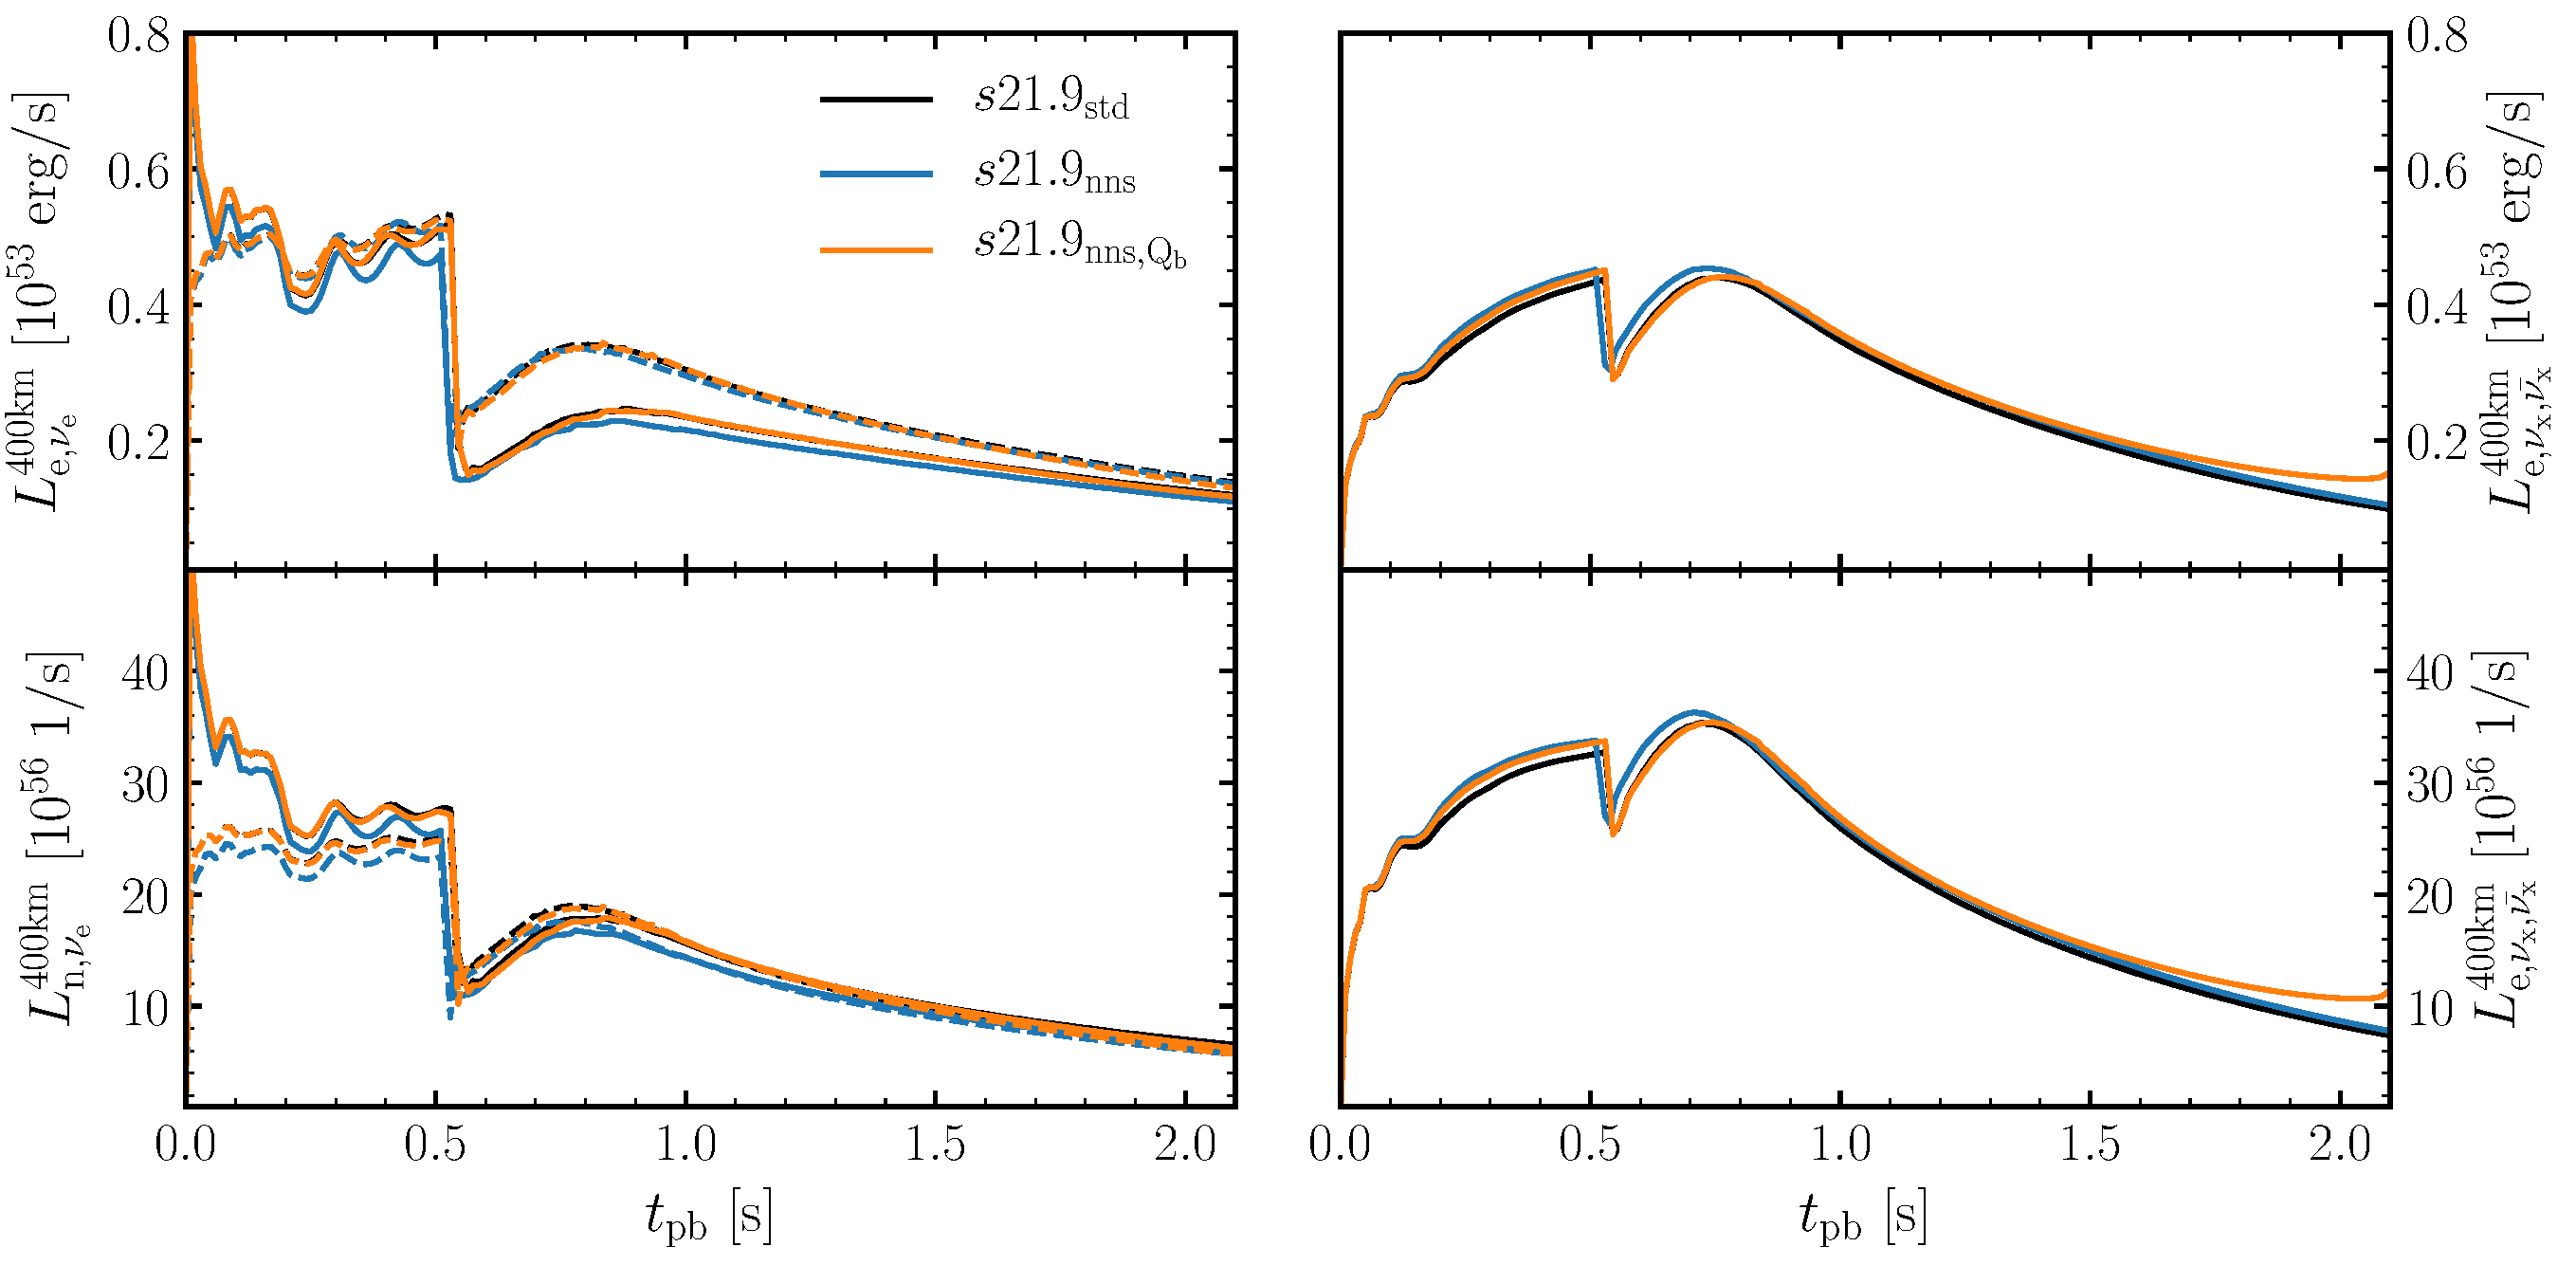
\includegraphics[width=0.8\textwidth]{./pic/s21_9_trans_tests.pdf}
 \caption{Neutrino energy and number luminosities for a $21.9\;\mathrm{M_{\odot}}$ star using the transport of S06 ($s21.9_{\mathrm{std}}$), the corrected transport ($s21.9_{\mathrm{nns}}$) and including Bremsstrahlung ($s21.9_{\mathrm{std,Q_b}}$). \textit{Upper left panel}: Electron neutrino (solid lines) and electron anti-neutrino energy-luminosity at $400\;\mathrm{km}$. \textit{Lower left panel}: Electron neutrino (solid lines) and electron anti-neutrino number-luminosity at $400\;\mathrm{km}$. The left column of panels shows the same quantities for the heavy neutrinos ($\nu_{\mathrm{x}}$). Including the corrections presented here reduces the overall luminosities for this model. Adding Bremsstrahlung somewhat balances the reduction of $L_{\mathrm{e,n},\nu}$}
 \label{fig:s21.9_tras}
\end{figure*}

 \subsection{Bremsstrahlung}

 In addition to the aforementioned improvements we now include neutrino Bremsstrahlung into our transport scheme. We follow the prescription given in \cite{BurrowsEtAl2006}.
 The total volumetric energy gain by heavy-lepton neutrinos by Nucleon-Nucleon Bremsstrahlung pair events, using the matter temperature $T$ and mass fractions $X_{\mathrm{n}}$, is given by

\begin{equation}
    Q_{\mathrm{nb}}^{\mathrm{\nu_i}} = 0.5\cdot 1.04\cdot 10^{30} \xi \; \big(X_{\mathrm{n}}\rho_{14}\big)^2 (\frac{T}{\mathrm{MeV}})^{5.5} \;\; [\frac{\mathrm{erg}}{\mathrm{cm^3s}}],
\end{equation}
where $\rho_{14} = \frac{\rho}{10^{14}} \mathrm{\frac{g}{cm^3}} $
and $X_{\mathrm{n}}^2$ is defined as
\begin{equation*}
 X_{\mathrm{n}}^2 = X_{\mathrm{neut}}^2 + X_{\mathrm{prot}}^2 + 28/3\; X_{\mathrm{neut}}X_{\mathrm{prot}}.
\end{equation*}

We add a factor of 0.5 in the above description as we calculate the energy generation by \textbf{one} neutrino and not by pairs of neutrinos. Here $\xi$ is a correction factor also set to 0.5.
For the energy loss we assume
\begin{equation}
    \frac{\kappa}{n_{\mathrm{b}}} = \frac{Q_{\mathrm{nb}}^{\mathrm{\nu_i}}}{c \epsilon^{\mathrm{eq}}} = \frac{Q_{\mathrm{nb}}^{-}\cdot 4\pi r^2 f_{\nu}}{L_{\nu}^{\mathrm{e}}}
\end{equation}
In the notation of S06 this becomes
\begin{equation}
    Q_{\mathrm{nb}}^{-} = \frac{Q_{\mathrm{nb}}^{\mathrm{\nu_i}} L_{\nu}^{\mathrm{e}} }{4\pi r^2 f_{\nu} c \epsilon^{\mathrm{eq}} n_{\mathrm{b}}}.
\end{equation}
For the Number emission we take
\begin{equation}
    R=\frac{Q_{\mathrm{nb}}^{\nu_{\mathrm{i}}}}{\langle \epsilon \rangle} = Q_{\mathrm{nb}}^{\nu_i} \frac{L_{\nu}^n }{L_{\nu}^e }\;\; \mathrm{\frac{1}{cm^3s}}
\end{equation}
and for the absorption taking $ n^{\mathrm{eq}}$ instead of $ \epsilon^{\mathrm{eq}} $ giving
\begin{equation}
    n^{\mathrm{eq}} = \frac{8\pi T^3}{(hc)^3}\mathrm{F}_2.
\end{equation}
Here $\mathrm{F}_2$ is the Fermi-Dirac integral defined in \autoref{equ:fermi-dirac-integral}.

%% TODO
%% SHOW TESTS
%% pair production should cool the material!
\end{appendices}
%-----------
% BIB
% --------------
\bibliographystyle{mnras}
\bibliography{ads-bibtex}       % name your BibTeX data base
\end{document}
% end of file template.tex

